\documentclass[letterpaper, paper,11pt]{AAS}	% for preprint proceedings
\usepackage{bm}
\usepackage{amsmath}
\usepackage{subfigure}
%\usepackage[notref,notcite]{showkeys}  % use this to temporarily show labels
\usepackage[colorlinks=true, pdfstartview=FitV, linkcolor=black, citecolor= black, urlcolor= black]{hyperref}
\usepackage{overcite}
\usepackage{footnpag}			      	% make footnote symbols restart on each page
% \usepackage{listings}                   % Code Listings
\usepackage[table, x11names]{xcolor}                     % Code Coloring
\usepackage{xfrac}                      % Slanted Fractions
\usepackage{booktabs}                   % Table Styling
\usepackage{multirow}                   % Table Styling
\usepackage{tikz}
\usepackage{tikz-3dplot}
\usepackage{hyperref}

% DEFINING CODE COLORS
% \definecolor{comments}{rgb}{0.0, 0.5z, 0.0}
% \definecolor{keywords}{rgb}{0.01, 0.28, 1}

% ADDITIONAL COMMANDS
\newcommand*\circled[1]{\tikz[baseline=(char.base)]{
            \node[shape=circle,draw,inner sep=0.8pt] (char) {#1};}}

% \lstset{
%     basicstyle = \small\ttfamily,
%     language = Python,
%     frame = lines,
%     backgroundcolor = \color{lightgray!10},
%     commentstyle = \color{comments}\ttfamily\small,
%     keywordstyle = \color{keywords}\bf\ttfamily\small,
%     framesep=\fboxsep,
% }

\PaperNumber{21-581}

\begin{document} 
% \setcounter{page}{5199} % For use when adding to publication

\title{MULTI-REVOLUTION EXTENSION OF SOLAR-PERTURBED MOON-TO-MOON TRANSFER FAMILIES}

\author{Burton Yale\thanks{Mission Design Intern, Mission Design and Navigation Section, Jet Propulsion Laboratory, California Institute of
Technology, M/S: 301-121, 4800 Oak Grove Dr., Pasadena, CA 91109.}\; and 
    Gregory Lantoine\thanks{Mission Design Engineer, Mission Design and Navigation Section, Jet Propulsion Laboratory, California Institute of
Technology, M/S: 301-121, 4800 Oak Grove Dr., Pasadena, CA 91109.}}

\maketitle{}

\begin{abstract}
Lunar flybys and solar perturbations present a golden opportunity to naturally modify trajectories of spacecraft launched in Moon-bound orbits. Leveraging the energy gained, or lost, from lunar flybys and multi-body effects allows for spacecraft to reach destinations not previously within their designed \(\Delta \)v budgets. Previous research studies have demonstrated the viability of collecting zero revolution Moon-to-Moon transfers into a referential database. This paper extends this capability to multi-revolution transfers and describes their main characteristics and increased versatility. Finally, a trajectory example is given for the escape phase of the NEA Scout mission.
\end{abstract}

\section*{Introduction}
\pdfbookmark[1]{Introduction}{motiv}

% {\color{cyan} Add larger discussion of previous results and some background on the three body problem and lunar gateway idea}

Ridesharing missions are not a new phenomenon among the small-sat community, but most of these programs are limited to LEO or GEO transfer orbits. With the prospective uptick in lunar-bound missions lies a new field of opportunities for large and small satellite operators. Multiple lunar flybys can allow spacecraft to gain orbital energy at little to no cost. Combined with solar perturbations at the edge of the Earth-Moon system, a spacecraft previously bound to this system can escape into heliocentric space~\cite{Mcelrath2012, Yarnoz2016, Chen2016, Chen2017}. These escape trajectories will be the focus of this paper, but are not the only use case for these solar-perturbed lunar flybys. For instance, spacecraft entering the Earth-Moon system can have their energy lowered in order to alleviate capture \(\Delta\)v requirements.

Due to third-body solar perturbations, these transfers require slower propagators compared to closed-form two-body systems, which hamper the mission design process if calculated individually for each use case. Instead, we can parameterize these orbits with a series of design variables. By pre-computing and storing these solutions within a database, they can be referenced without the need for repropagation, therefore reducing the run time by orders of magnitude. This advantage, it allows for the design and optimization of multiple candidate trajectories at a higher rate with a smaller human-in-the-loop requirement.

The previous paper in this series has completed the exploration of zero-revolution transfers~\cite{Lantoine2014}. However, there is still room for improvements upon this dataset. In fact, for higher time of flights for Moon-to-Moon transfers, a spacecraft can spend more time at the edges of the Earth-Moon system, thus solar perturbations can take a larger and larger effect on the spacecraft's path. These increased solar perturbations tend to narrow the regions where these orbits are possible, creating gaps. By expanding the trajectory space to multi-revolution transfers, these gaps can be shrunk. As a result, a larger variety of trajectories can be found that meet mission constraints, allowing for higher flexibility for a mission designer.

\section*{Methods and Models}
\pdfbookmark[1]{Methods and Models}{methods}

% {\color{cyan} Explain design variables more, new pictures for steps

% Show visual for different families and subtypes

% Show how multi-rev orbits are defined}

The primary purpose of this paper is to develop a roadmap for finding and extending Moon-to-Moon transfers to multi-revolution regimes. As discussed previously, primary model to be used for this analysis will be the Sun-Earth Circular Restricted Three-Body Problem (CR3BP). Additionally, as these orbits will be parameterized, a naming convention is necessary that can conveniently and concisely dictate which orbit is being used.

For the following equations, bolded variables indicate vector notation, while non-bolded variables are scalar in nature. Similarly, variables subscripted by \(S\), \(M\), and \(E\) refer to the Sun, Moon, and Earth respectively.

\subsection*{Environment Definition}
\pdfbookmark[2]{Environment Definition}{env}

In short, the CR3BP describes the motion of a sufficiently small body within the influence of two larger bodies, one orbiting another on a circular path. For this paper, the larger of two bodies will be the Sun, and the smaller being the Earth. 

\begin{figure}[h]
    \centering
    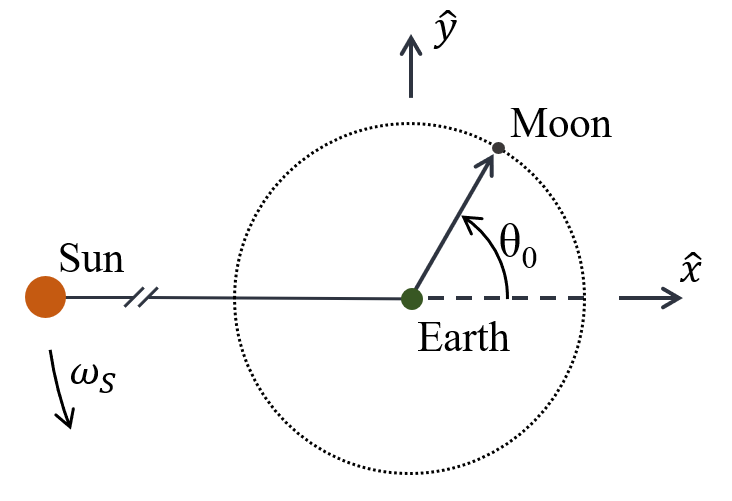
\includegraphics[width=4in]{./figs/diag_sunearth.png}
    \caption{Coordinate frame definition for the trajectories within this paper. It should be noted that the Sun can rotate freely, and only inline with the negative x-axis at \(t_0\).}
    \label{fig:sunearth}
\end{figure}

To further simplify the problem, the Moon is assumed to be massless. Furthermore, the Sun, Earth, and Moon are assumed to have coplanar orbits, as the actual plane difference is small (\(\sim\)5 deg). Additionally, we assume that the Moon's orbit around the Earth is circular, and current position is defined by the value of \(\theta\). This angle is defined from the x-axis vector created by the vector connecting the Sun and Earth in the environments initial state at zero time, as shown in Figure~\ref{fig:sunearth}. The motion of the spacecraft in this system can be described by the following differential equation:
\begin{equation}
    \ddot{\mathbf{R}} = -\mu_E\frac{ \mathbf{R} }{ \Vert\mathbf{R}\Vert^3 } - \mu_S\left( \frac{\mathbf{R} - \mathbf{R}_S}{\Vert\mathbf{R}-\mathbf{R}_S\Vert^3} + \frac{ \mathbf{R}_S }{ \Vert\mathbf{R}_S\Vert^3 } \right)
    \label{eq:EOM}
\end{equation}

Different from the standard, normalized equations of motion in a rotating frame, this model represents an inertial, non-rotating center at Earth, rather than at the system barycenter. As such, the spacecrafts position, represented by \(\mathbf{R}\), is acted on by the normal two-body equation of motion in the first term plus a perturbing factor. This factor being the gravitational influence of the Sun rotating around the Earth center, represented by \(\mathbf{R}_S\). More precisely, the Sun position can be found with the following expressions, the first, \(\omega_S\), being the circular orbit rotational rate of the body around the Earth.

\begin{equation}
    \omega_S = \sqrt{\frac{\mu_S + \mu_E}{r_S^3}}
    \label{eq:omS}
\end{equation}

\begin{equation}
    \mathbf{R}_S = -R_S[\cos(\omega_S\, t), \sin(\omega_S\, t), 0]
    \label{eq:RS}
\end{equation}

When constructing the initial conditions for Moon-to-Moon transfers, all orbits are considered to start on a Lunar, two-body, hyperbolic trajectory, whose coordinates are defined in spherical notation on the v\(_\infty\) globe~\cite{Strange2008}. Additionally, all vectors are defined in a rotating frame derived from the, assumed, circular motion around the Earth, as represented in Figure~\ref{fig:mooncoords}.

\begin{figure}[h]
    \centering
    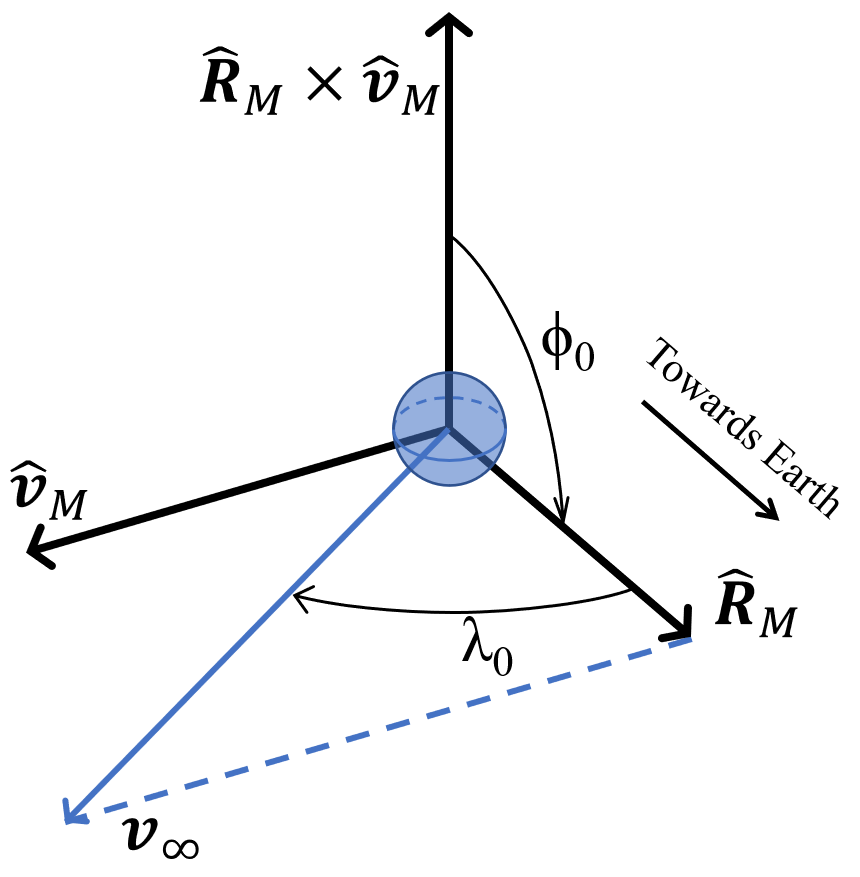
\includegraphics[width=3in]{./figs/diag_moon.png}
    \caption{Departure definitions for spacecraft integration initial conditions within the Lunar two-body system.}
    \label{fig:mooncoords}
\end{figure}

With \(\lambda_0\) denoting the latitude of the \textbf{v}\(_\infty\) departure vector measured from the component of the \textbf{v}\(_\infty\) along the \(\hat{\mathbf{R}}_M\) direction. Defining the direction of the \textbf{v}\(_\infty\) along the \(\hat{\mathbf{R}}_M\) direction, positive or negative, is the longitude of the departure, \(\phi_0\) measured from the angular momentum vector pointing out of plane. To convert these rotating coordinates into inertial, Earth-centered coordinates used by the equations of motion, we first must define the motion of the Moon around the Earth. Using the following equations we arrive at the definitions for the circular orbit:

\begin{equation}
    \omega_M = \sqrt{\frac{\mu_E + \mu_M}{r_M^3}}
    \label{eq:omM}
\end{equation}

\begin{equation}
    \mathbf{R}_M = R_M[\cos(\omega_M\, t), \sin(\omega_M\, t), 0]
    \label{eq:RM}
\end{equation}

\begin{equation}
    \mathbf{v}_M = \sqrt{\frac{\mu_E + \mu_M}{r_M}}[-\sin(\omega_M\, t), \cos(\omega_M\, t), 0]
    \label{eq:vM}
\end{equation}

Combining Equations~\ref{eq:omM}-\ref{eq:vM} and the variables we defined in Figure~\ref{fig:mooncoords}, we arrive at a method to transcribe escape vectors on the \textbf{v}\(_\infty\) globe into initial conditions for the integration of the trajectory:

\begin{equation}
    \mathbf{v}_0 = v_\infty\cos(\lambda)\sin(\phi)\hat{\mathbf{R}}_M + (v_M + v_\infty\sin(\lambda))\hat{\mathbf{v}}_M
    \label{eq:vIC}
\end{equation}

Collecting all of the above variables used to describe the motion of the spacecraft, we arrive at a total of six values that uniquely define each Moon-to-Moon trajectory. Including time of flight, the below table contains a list of all variables, their symbols, and necessary descriptions:

\begin{table}[h]
    \centering
    \caption{Moon-to-Moon transfer design variables used to categorize and define trajectories.}
    \label{tab:my-table}
    \begin{tabular}{lcl}
        \toprule
        \textbf{Name} & \textbf{Variable} & \textbf{Description} \\
        \midrule
        Departure Solar Phase Angle      & \(\theta_0\)  & \parbox{7.5cm}{The three-body angle between the Sun, Earth, and Moon.} \\[0.5cm]
        Time of Flight                   & \(TOF\)       & \parbox{7.5cm}{Transfer time between lunar encounters and is one of the key elements to be optimized when finding transfers.} \\[0.7cm]
        Departure Lunar Escape Velocity  & v\(_\infty\)  & \parbox{7.5cm}{The scalar hyperbolic excess velocity on the outbound encounter with the Moon.} \\[0.5cm]
        Departure v\(_\infty\) Longitude & \(\phi_0\)    & \parbox{7.5cm}{The departure longitude, on the v\(_\infty\) globe~\cite{Strange2008}. Discrete values of either -90° or 90°, determines whether the outbound transfer is inward or outward facing, respectively.} \\[1cm]
        Arrival v\(_\infty\) Longitude   & \(\phi_f\)    & \parbox{7.5cm}{Similarly, the arrival longitude, determines the inbound transfer is in-ward or outward facing.} \\[0.5cm]
        Departure v\(_\infty\) Latitude  & \(\lambda_0\) & \parbox{7.5cm}{The departure latitude, on the v\(_\infty\) globe.~\cite{Strange2008}. Continuous values from -90° to 90°, the other key value to be optimized when finding transfers.} \\
        \bottomrule
    \end{tabular}
\end{table}

\subsection*{Nomenclature}
\pdfbookmark[2]{Nomenclature}{names}

Before beginning the methodology of finding families of Moon-to-Moon transfers, we must first develop a categorization method to accurately and quickly describe each transfer. There are many methods of doing so, but the method decided upon in this paper will be to have each trajectory fall into a hierarchy by their total time of flight from each Lunar orbit crossing. For each month in time of flight, also roughly coinciding with the orbital period of the Moon, is encoded with a letter A-Z. For example, a 30 day, one month, transfer would receive and A designation while a 112 day transfer would get a D designation.

% {\color{cyan}Picture showing progression of orbits over time of flight}

These groups are further sub-divided by the initial and final v\(_\infty\) longitudes (\(\phi_0\) and \(\phi_f\)). Longitudes with a value of -90° are subscripted \emph{i} for inward flying orbits, and 90° are subscripted \emph{o} for outward flying orbits. Examples of all four possibilities are described in Figure~\ref{fig:subtypes}. By combining both definitions, we arrive at a naming convention that defines all possible varieties of Moon-to-Moon transfers. As families exhibit similar trajectory structures for the roughly the same values of time of flights for a given beginning and end condition. These structures persist even when changing the values of the launch v\(_\infty\), and as such, is not a primary contributor to the naming convention. Examples of this full definition could be Aii, Bio, Coi, Doo, etc., and for time of flight A-F, there exists 24 total families of orbit classes, four sub-classes for each time of flight bracket.

\begin{figure}[h]
    \centering
    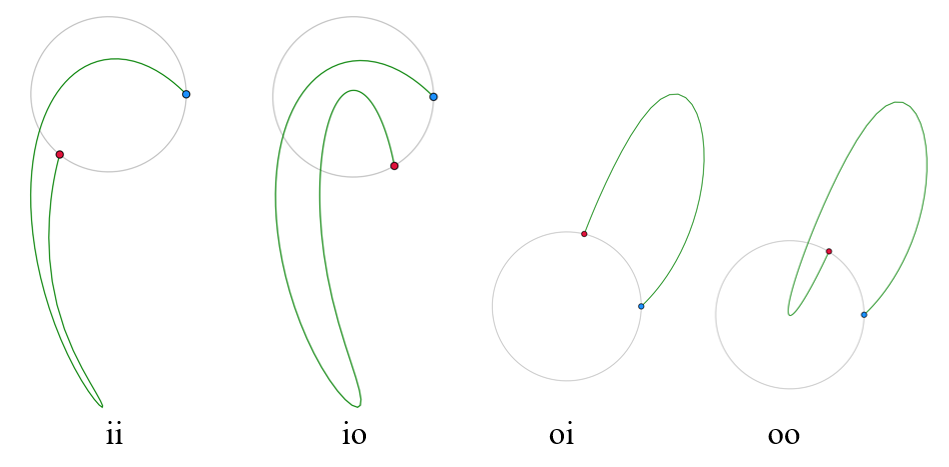
\includegraphics[width=4in]{./etc/src (3).png}
    \caption{All four subtypes of Moon-to-Moon trajectories. Note all trajectories originate blue mark at 0°, and terminate at the red mark.}%\(^\mathbf{*}\)}
    \label{fig:subtypes}
\end{figure}

% \footnotetext[1]{Images are for illustration purposes and may or may not exist within the dataset}

When extending this definition to multi-revolution transfers, a modification of the month-wise time of flight definition is required. To keep in line with the previous naming scheme, each revolution of the orbit will be considered for the beginning of each family name. For example, a transfer with the first orbit being 2-months, and the second being 4-months would be an BD transfer. The boundary for each revolution is defined by the targeted arrival v\(_\infty\) longitude, as shown in Figure~\ref{fig:revs}. A special condition exists where the orbit does not cross the lunar orbital radius. When such a situation occurs, the next lowest radius in the orbit is considered as the break point.


\begin{figure}[h]
    \centering
    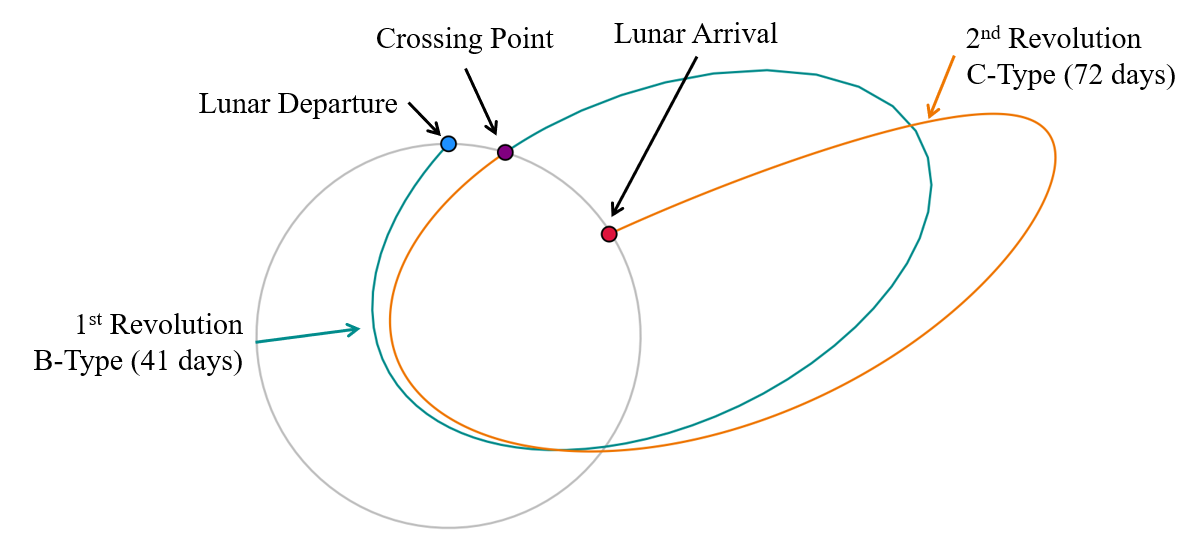
\includegraphics[trim=0 10 0 10, clip, width=4.2in]{./etc/src (1).png}
    \caption{Major components of a multi-revolution trajectory.}%\(^\mathbf{*}\)}
    \label{fig:revs}
\end{figure}

% {\color{cyan} Show boundary and special condition using trajectory plot}

\subsection*{Solving for Trajectory Families}
\pdfbookmark[2]{Solving for Trajectory Families}{fams}

With these definitions in mind, now we can move onto the steps involved in generating the Moon-to-Moon families. Generating each family follows the same procedure, as depicted below in Figure~\ref{fig:flow}.

\begin{figure}[h]
    \centering
    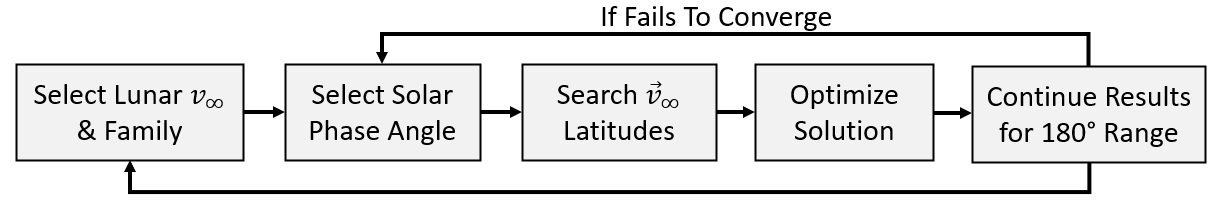
\includegraphics[width=5in]{./etc/src (2).png}
    \caption{Flow diagram for converging and generating Moon-To-Moon trajectory families.}%\(^\mathbf{*}\)}
    \label{fig:flow}
\end{figure}

When initiating a search, in order to limit the search space, we will choose a specific family, for example Dio. With a family selected the next step is selecting a v\(_\infty\) for the spacecraft to launch from the Moon with. Most trajectories will reside in the range of 0.3 \(^{km}/_s\) to 2.2 \(^{km}/_s\)~\cite{Lantoine2014}.

The next values to access is the solar phase angle, \(\theta_0\), and launch latitudes, \(\lambda_0\). Starting with an initial \(\theta_0\) of 0°, a range of departure latitudes are selected for testing possible transfers. Each latitude has its initial state integrated until either the maximum integration time for the family is met, or the spacecraft crosses the Moon's orbit the correct arrival conditions. Solutions that stop within 50,000 km or less of the Moon's position at that time are kept for future steps. When testing these ranges, it is important to have a sufficiently small step size, as these solutions exist only within tenths or twentieths of a degree, making searching the whole range of possibilities a slow task. It can be noted that the general ranges of latitudes, 20-30 degrees wide, where solutions are present persists between families of the same departure subscripts and v\(_\infty\). One possible example shown in Figure~\ref{fig:latitudesearch}.

\begin{figure}[h!]
    \centering
    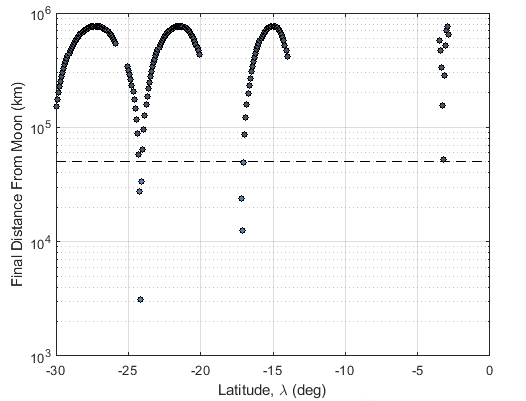
\includegraphics[width=4in]{./etc/latitudespace.png}
    \caption{A latitude range searched by the algorithm. Showing 2-rev, 1-rev, and 0-rev solutions at -24°, -18°, and -4° respectively. Solutions are trajectories that terminate at a distance from the Moon below the dotted line at 50,000 km.}
    \label{fig:latitudesearch}
\end{figure}
%The launch conditions are then integrated until a stop condition is met, either running out of integration time, or meeting the Moon’s orbit with the correct velocity direction. The final position of the integration is compared against the positions of the Moon after the corresponding time has elapsed. These values can be plotted, as in {\color{red}Figure 3}. Over a range of 30°, the required launch latitudes for 2, 1, and 0 revolution transfer can be found. It should be noted that not all transfers are required to exist at any given combination of v\(_\infty\) and \(\theta_0\). We will be selecting the 1-revolution family for the next steps. If no trajectory is found, a new \(\theta_0\) is selected until a solution is found.

Once a solution has been selected, a two-dimensional differential corrector is used to bring the final distance between the Moon and the spacecraft to within acceptable tolerances~\cite{Lantoine2014}. The state variables used for this varying this trajectory are the launch latitude and total time of flight of the trajectory. Solution optimization of 1-revolution transfer shown in Figure~\ref{fig:optimization}.

With the initial trajectory optimized, the solution is then continued bidirectionally from its origin point by stepping the previous solution’s initial solar phase angle a small amount and reoptimizing the solution. This continues either until the solutions begin to diverge, or the entire continued solution spans 180°. In case of lack of convergence, a new search begins to find a seed trajectory with a different solar phase angle, using the same method as described above.

Once the span has been searched and/or continued, the key parameters from the results are stored for future reference. These values eliminate the need for re-integration when referencing different trajectory types. In order to link together these families, all that is required is the beginning and end v\(_\infty\) vectors to compute a two-body flyby about the Moon.

\begin{figure}[h!]
    \centering
    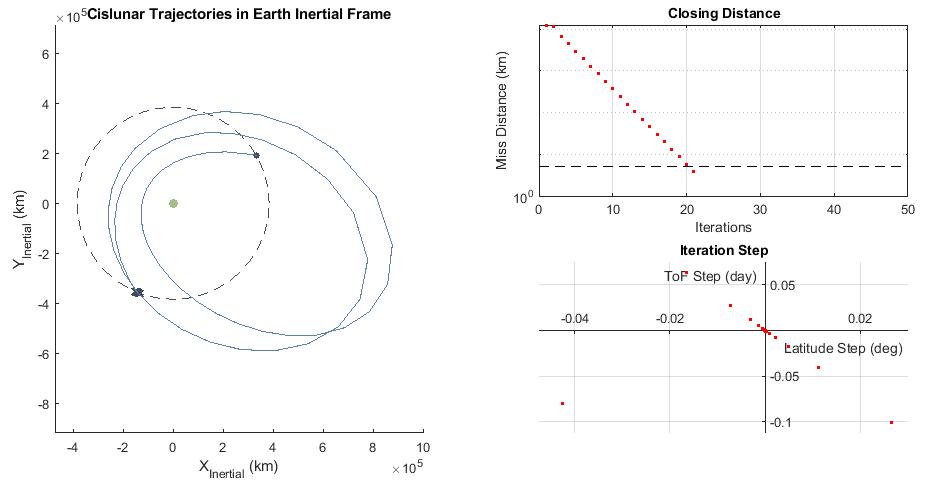
\includegraphics[width=6in]{./etc/optimization.png}
    \caption{Optimization of 1-rev io trajectory showing closing distance and steps with each iteration converging to a solution. The step each iteration takes, shown in the bottom right, shows the optimizer honing in on the path to an optimized solution, slowly decreasing its step size until bounds are met.}
    \label{fig:optimization}
\end{figure} 

\section*{Results}
\pdfbookmark[1]{Results}{results}

Apart from the use case of quick trajectory design, taking a step back can reveal trends among the datasets that set these multi-revolution orbits apart from their zero revolution counterparts. For the purpose of entering heliocentric space, multi-revolution families of the same time of flight have lower energy than their counterparts which can lengthen total mission time. This is primarily down to fact that lower revolution transfers need to be in a higher energy state, thus spending more time at the outer bounds of system, to achieve the same time of flight as a multi-revolution transfer, which can simply do more revolutions at a closer proximity to the center body. This can also be a benefit in terms of "loitering" in cislunar space while the encounter waits to present itself. As is the nature with ride-share missions, choosing the exact epoch of departure is not an ideal condition. The flexibility of extending a certain part of the mission to still meet mission constraints is one of the major viabilities of multi-revolution trajectories. 

Taking a closer look at direct similarities, multi-revolutions orbits also tend to span higher solar phase angles for the same level of time of flight, as shown in Figure~\ref{fig:tof_comparison}. The zero-revolution families quickly begin to taper off in terms of coverage, decreasing to roughly 40°, while the multi-revolution families continue to cover most of the possible solar phase angles. Another trend among the data is the tendency for zero-revolution data to exist where the multi-revolution data does not. This can be clearly seen in Figure~\ref{fig:tof_comparison}, where the Doi multi-revolution coverage falls out between 30° and 90°, while zero-revolution data exists within that space.  %For the F families, zero-revolution orbits span roughly 40° while multi-revolution orbits span nearly 120°. Another advantage for including multi-body orbits is that when combined with the coverage of zero-revolution orbits, they tend to span the whole width of possible solar phase angles, especially at higher times of flight. As visible within the figure, the left hand orbits span from approximately 50° to 100°, while there is a gap on the right hand plot that can contain those trajectories over the same range.

\begin{figure}[h]
    \centering
    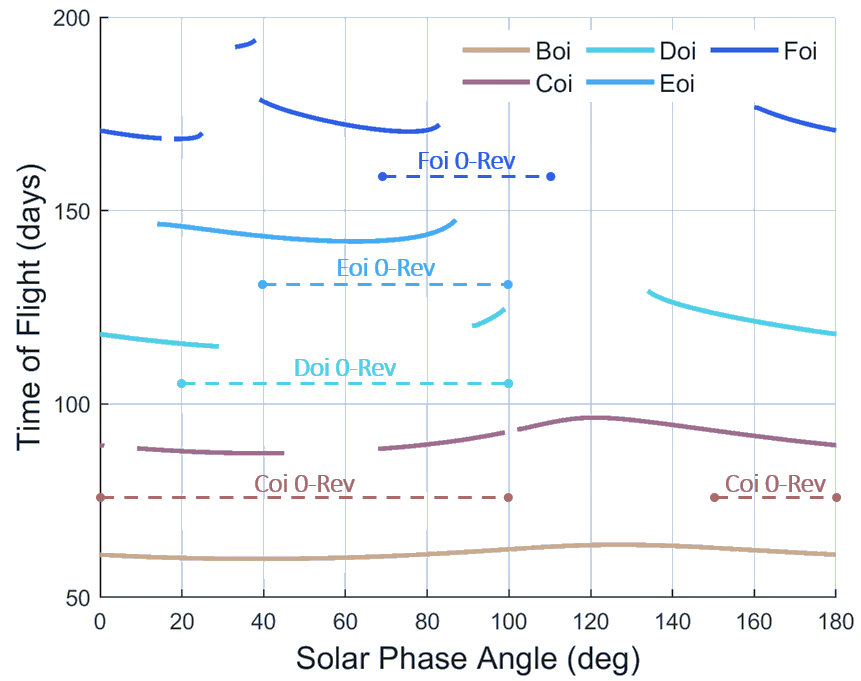
\includegraphics[width=4in]{./etc/spancompare.png}
    \caption{Spans of both zero-revolution transfers (dotted lines) and multi-revolution transfers (solid lines) for a v\(_\infty\) of 1.2\(^{km}/_s\). Note spans of zero-revolution transfers do not indicate time of flight, only coverage of Solar Phase Angle space.}
    \label{fig:tof_comparison}
\end{figure}

An additional property of note for cislunar trajectories is the ability to mirror trajectories with opposite starting conditions, as shown in Figure~\ref{fig:state_famoo_vinf0.6_tof} (Left). While the total possible solution space spans 360°, a pattern begins to emerge every 180° as the trajectory structures nearly repeat themselves. As the \(\mu\) of the Earth-Sun CR3BP system is very small (\(\sim\)3e-6), the dynamics at play are roughly approximate to those described in the Hill problem~\cite{Kalantonis2020}. Where the larger body, in this case the Sun, is infinitely far away while maintaining the same force over the whole system. This results in the gradient of the Sun's influence in the x-direction being negligible, exerting the same force at any distance. Thus, to get the mirrored solutions all one must do is rotate the initial and final conditions of the orbit, the \textbf{v}\(_{\infty, 0}\), \textbf{v}\(_{\infty, f}\), \(\theta_0\), and \(\theta_f\), by 180°. This doubles the number of pre-computed orbits in the database orbits without the need for reintegration of all the trajectories in the database.

For the sake of comparison, we have used, in Figure~\ref{fig:tof_comparison}, the same naming convention as in previous papers for both zero and multi-revolution orbits, but when discussing entire families of multi-revolution orbits, the single letter definitions do not let on to the real structure contained in these trajectories. At lower time of flights, there is little variation in the time of flight between revolutions, so naming schemes across solar phase angles remains relatively constant. As time of flight increases, there are often bifurcation points where the trajectory splits into multiple separate sub-families, as shown in Figure~\ref{fig:state_famoo_vinf0.6_tof}. A previously Foo family is split into CCoo, DBoo, and BDoo families. These branch points often occur in cases of singularities on close approach with the Earth, as well as with trajectory reversals out at the edges of the Earth-Moon system, where solar influence is maximized. An example of this kind of reversal is shown in the bottom left of Figure~\ref{fig:mooni_thetaPlot_io_E_2.1}, with cyan trajectory starts as a normal retrograde trajectory, then, in red, transitions to an orbit that starts the same, then flips prograde on one revolution and back to retrograde on the following. These flips are often the cause of discontinuities within the time of flight plots below.

\begin{figure}[h!]
    \centering
    \begin{subfigure}
        \centering
        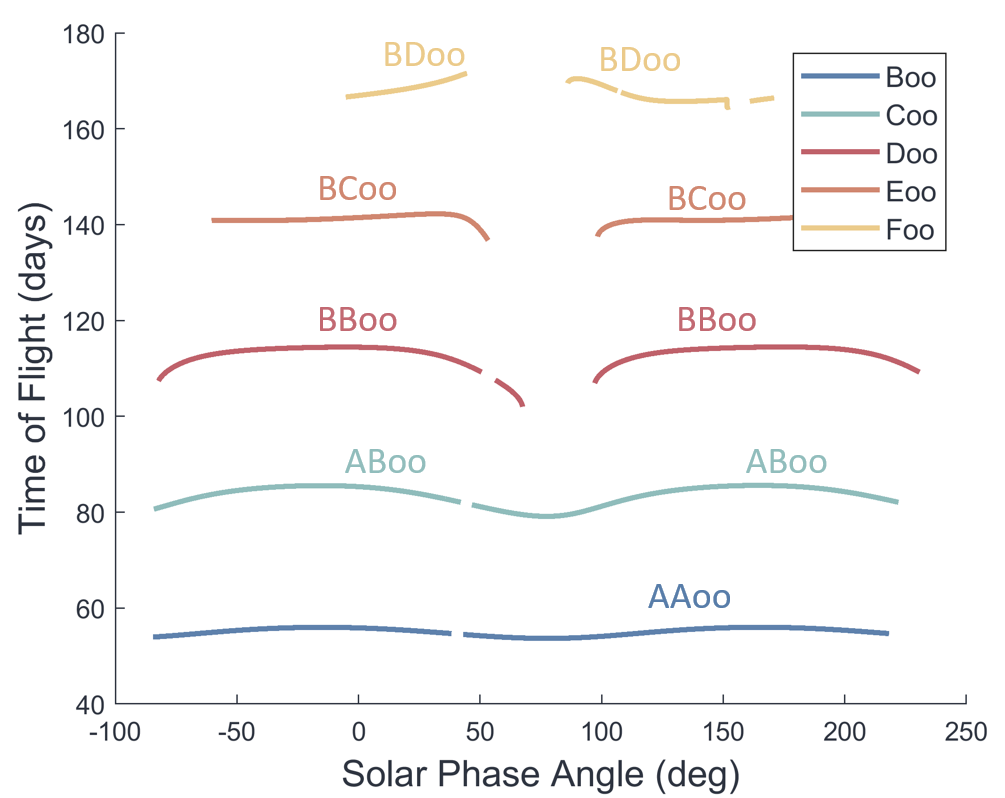
\includegraphics[width=2.75in]{./etc/names.png}     
    \end{subfigure}
    \begin{subfigure}
        \centering
        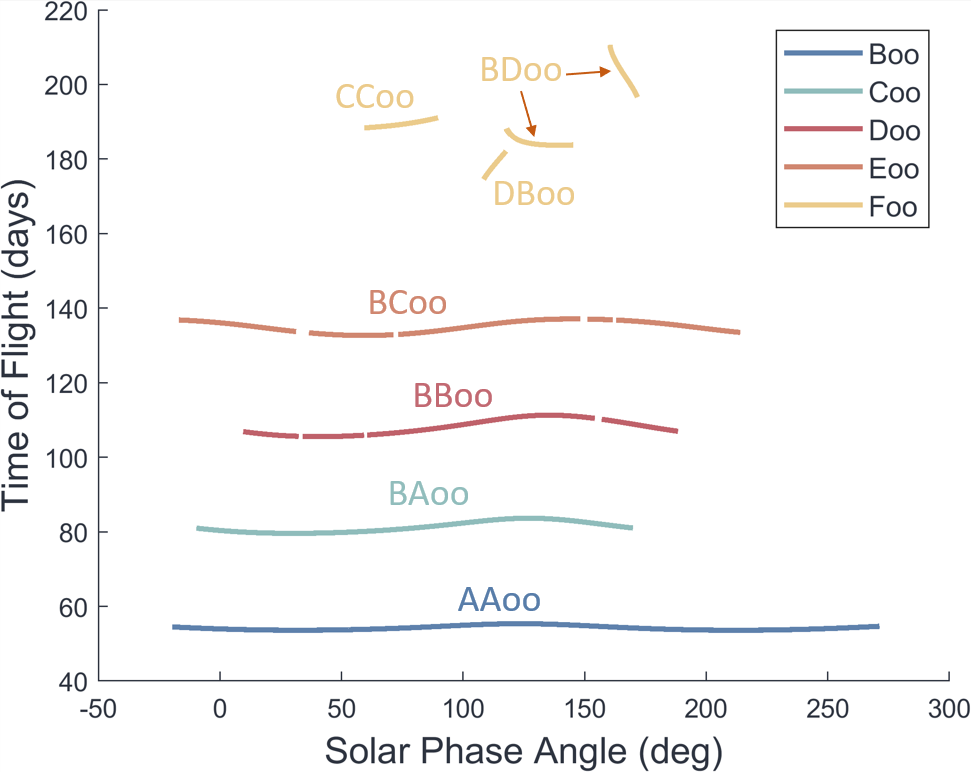
\includegraphics[width=2.75in]{./etc/names2.png}     
    \end{subfigure}
    \caption{Naming trajectory families by their multi-revolution names. (Left) "oo" families at a v\(_\infty\) of 0.6 \(^{km}/_s\). (Right) "oo" families at a v\(_\infty\) of 1.8 \(^{km}/_s\).}
    \label{fig:state_famoo_vinf0.6_tof}
\end{figure}

By varying the different parameters such as time of flight or launch v\(_\infty\) magnitude for the same remaining launch conditions, other patterns can emerge. Specifically when varying time of flight, and thus the family definition, as seen in Figure~\ref{fig:mooni_famPlot_oo_0.6}, the orbits exhibit similar overall structures but at different scales. For example, in the top left plot at \(\theta_0\) = 0°, there are two distinct loops in the orbits, one larger than the other. As time of flight increases, so do these loops, but also the distance between each loop. These revolutions start at roughly equal, AAoo, but progress to be nearly two "families" apart in time of flight, BDoo. While more prominent on non-zero \(\theta_0\), the rotation of each loop also increases as time of flight increases, due to large solar disturbances. The bottom plot of Figure~\ref{fig:mooni_famPlot_oo_0.6} shows that the rotation of orbits at the lowest and highest time of flight levels are nearly orthogonal to each other, and that the rotation between each revolution is more prominent. 

When varying v\(_\infty\), the changes in orbits are more drastic. In all cases the results are the same, as the velocity of departure increases, the orbit must become more and more retrograde to compensate. Specifically for orbits that start by travelling inward, such as \emph{ii} orbits, there exists a critical v\(_\infty\) where departure latitude is roughly 0°. This can cause many low altitude Earth approaches and singularity cases, leading to integration instabilities. These results can be found in Figure~\ref{fig:mooni_vinfPlot_io_C}.

Holding both time of flight and v\(_\infty\) constant, the changes in solar phase angle, \(\theta_0\), give rise to repetitive nature, previous discussed, in Moon-to-Moon trajectories, as seen in Figure~\ref{fig:mooni_thetaPlot_io_E_2.1}. These similarities become apparent in the first and last trajectories plotted (blue and orange arcs), as they lie roughly 180° apart. Since all trajectories are rotated so their initial position starts on the right side x-axis, regardless of \(\theta_0\) value, a bounded region is created where all trajectories must exist within. Sketched by the farthest point any trajectory reaches during propagation. These regions are also visible in the rotating frame in Appendix A Figure~\ref{fig:sunrot_thetaPlot_io_F_2.1}. %Figure~\ref{fig:mooni_thetaPlot_io_E_2.1}'s structures become more complicated as the variable iterated is the solar phase angle, \(\theta_0\), they exhibit a bounded region where all trajectories lie within. Since all trajectories are rotated so their initial position starts on the right side x-axis, regardless of \(\theta_0\) value, another standout property is again the repetitive nature of the orbits. For all plots, the first and last trajectories in the sequence (blue and orange arcs), all show similar shapes that can be blended into one another. 

\clearpage

\begin{figure}[h!]
    \begin{subfigure}{}
        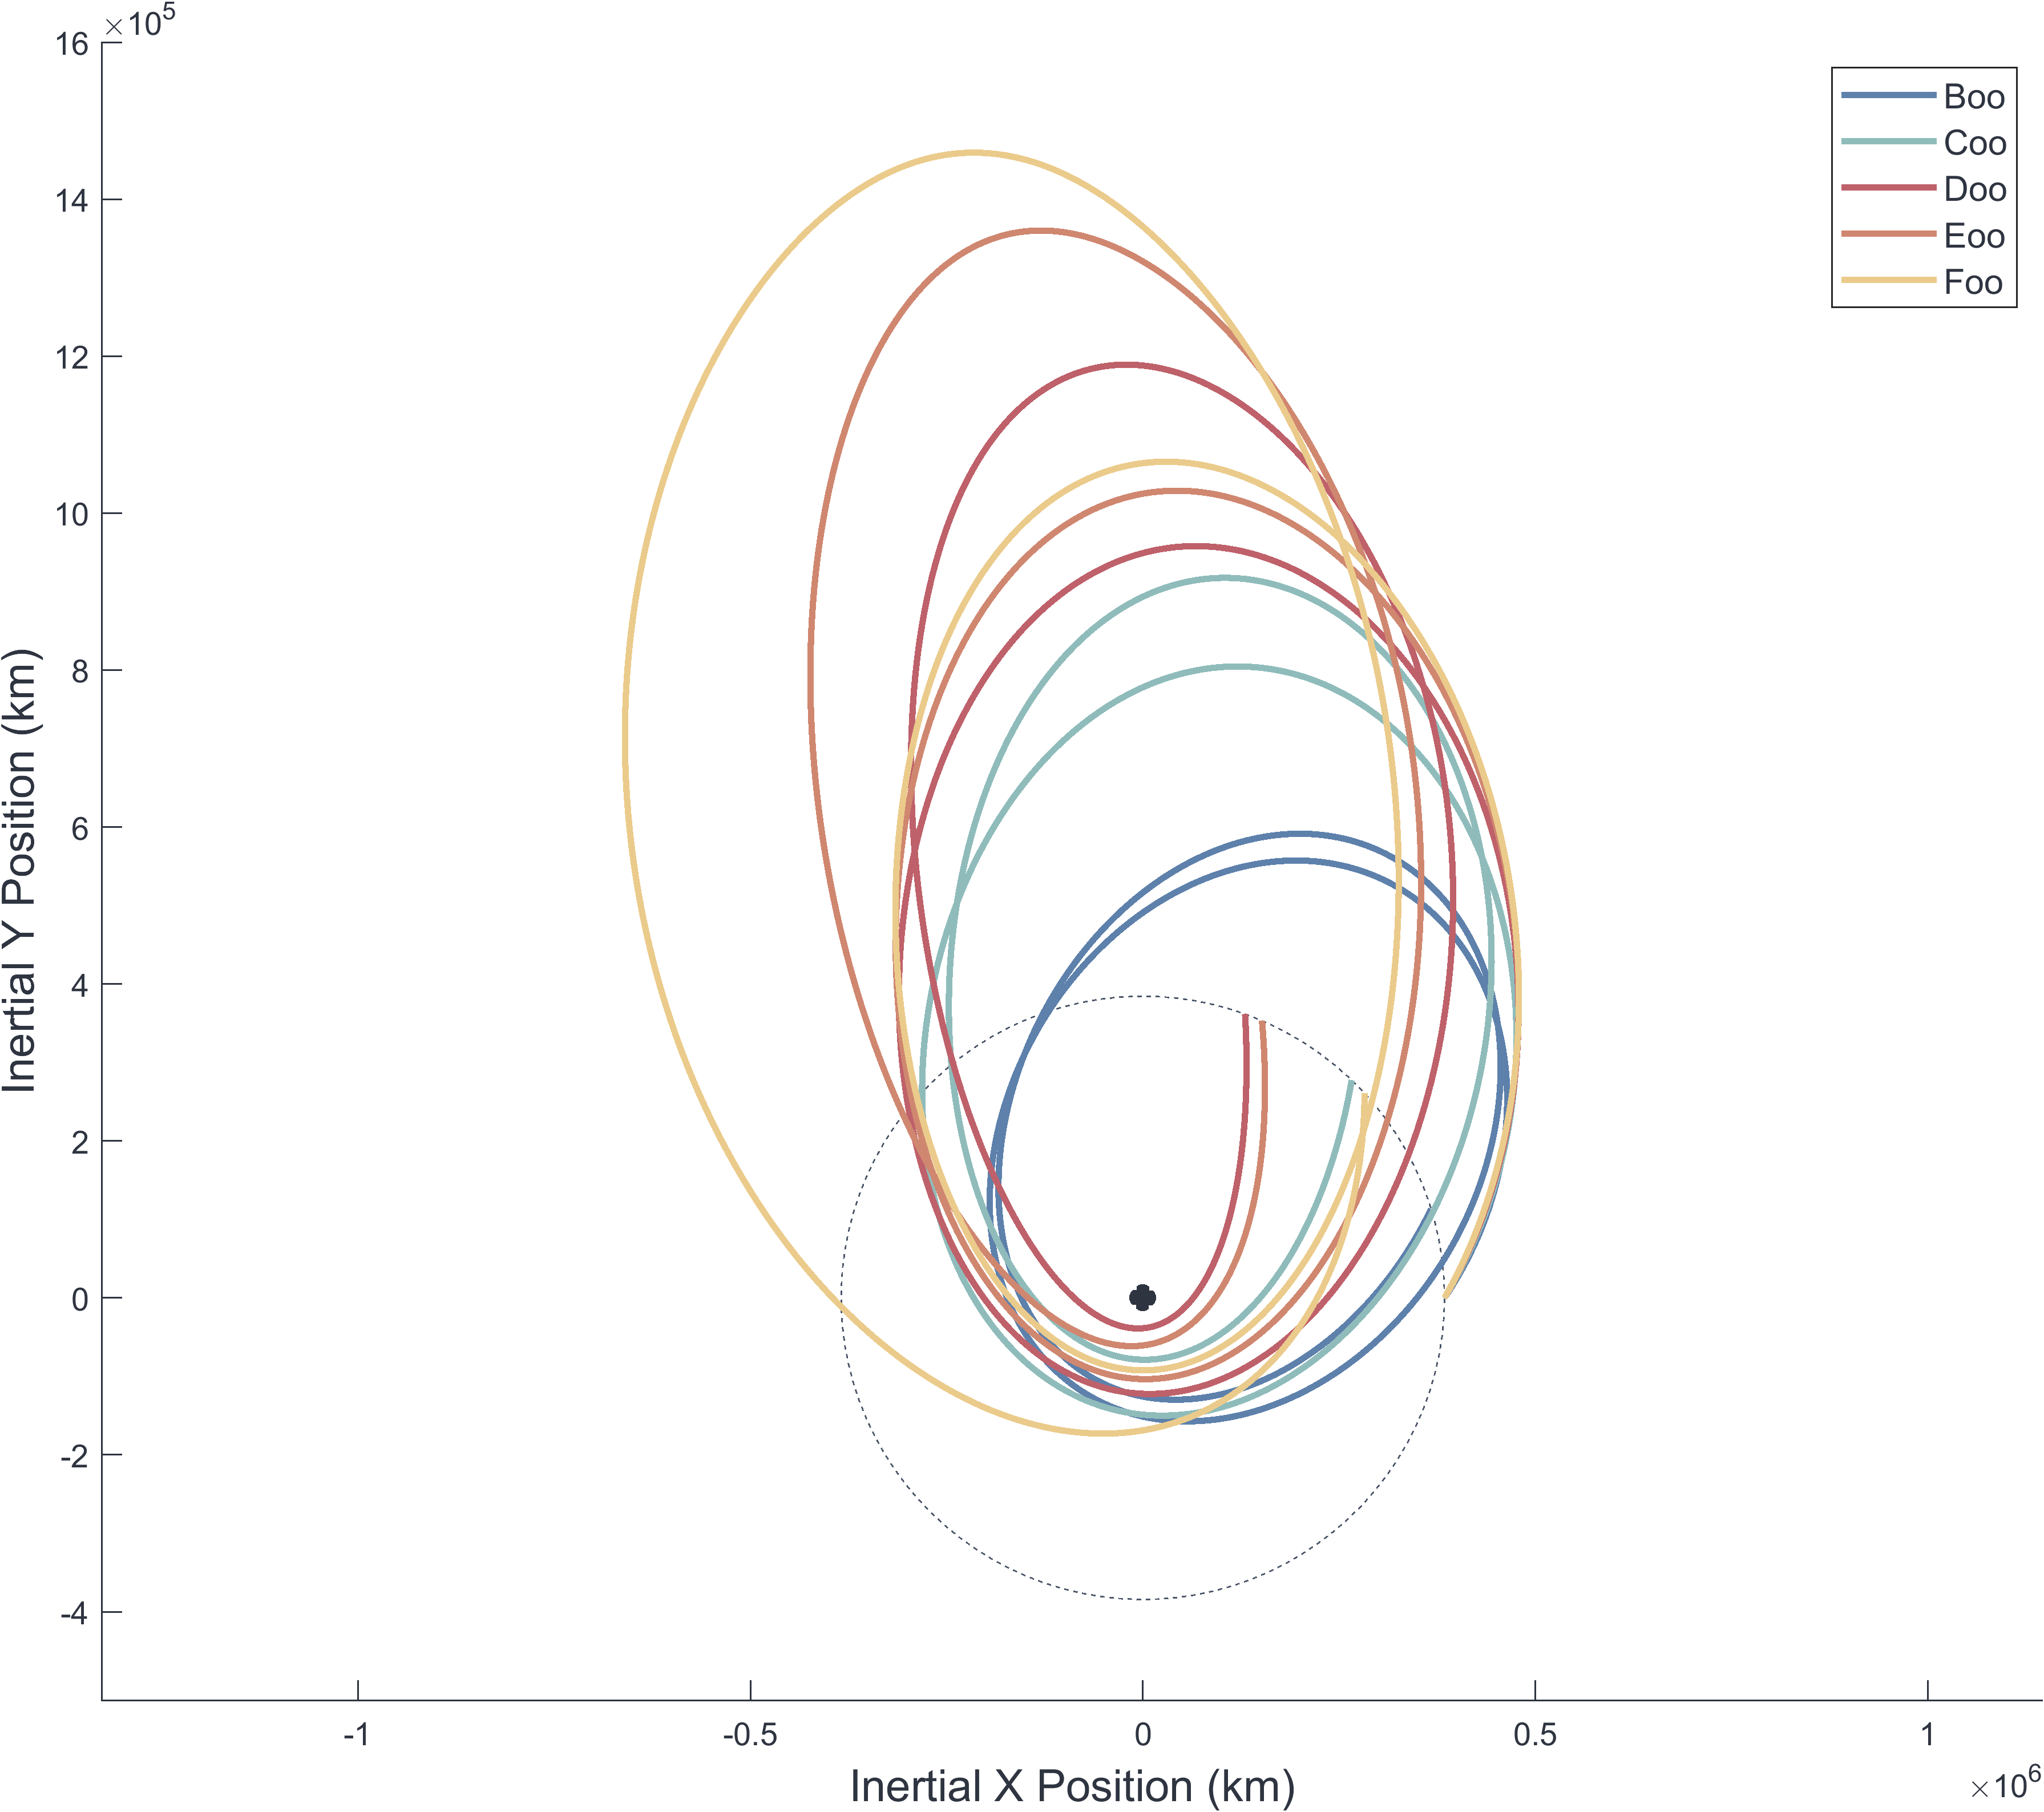
\includegraphics[trim=75 50 0 0, clip, width=3in]{./figs/mooni_FamilyPlot_oo_vInf0.6_theta0.png}
        % \caption{Top 25 results from Europa Clipper dataset, color sorted by sequence}
    \end{subfigure}
    \begin{subfigure}{}
        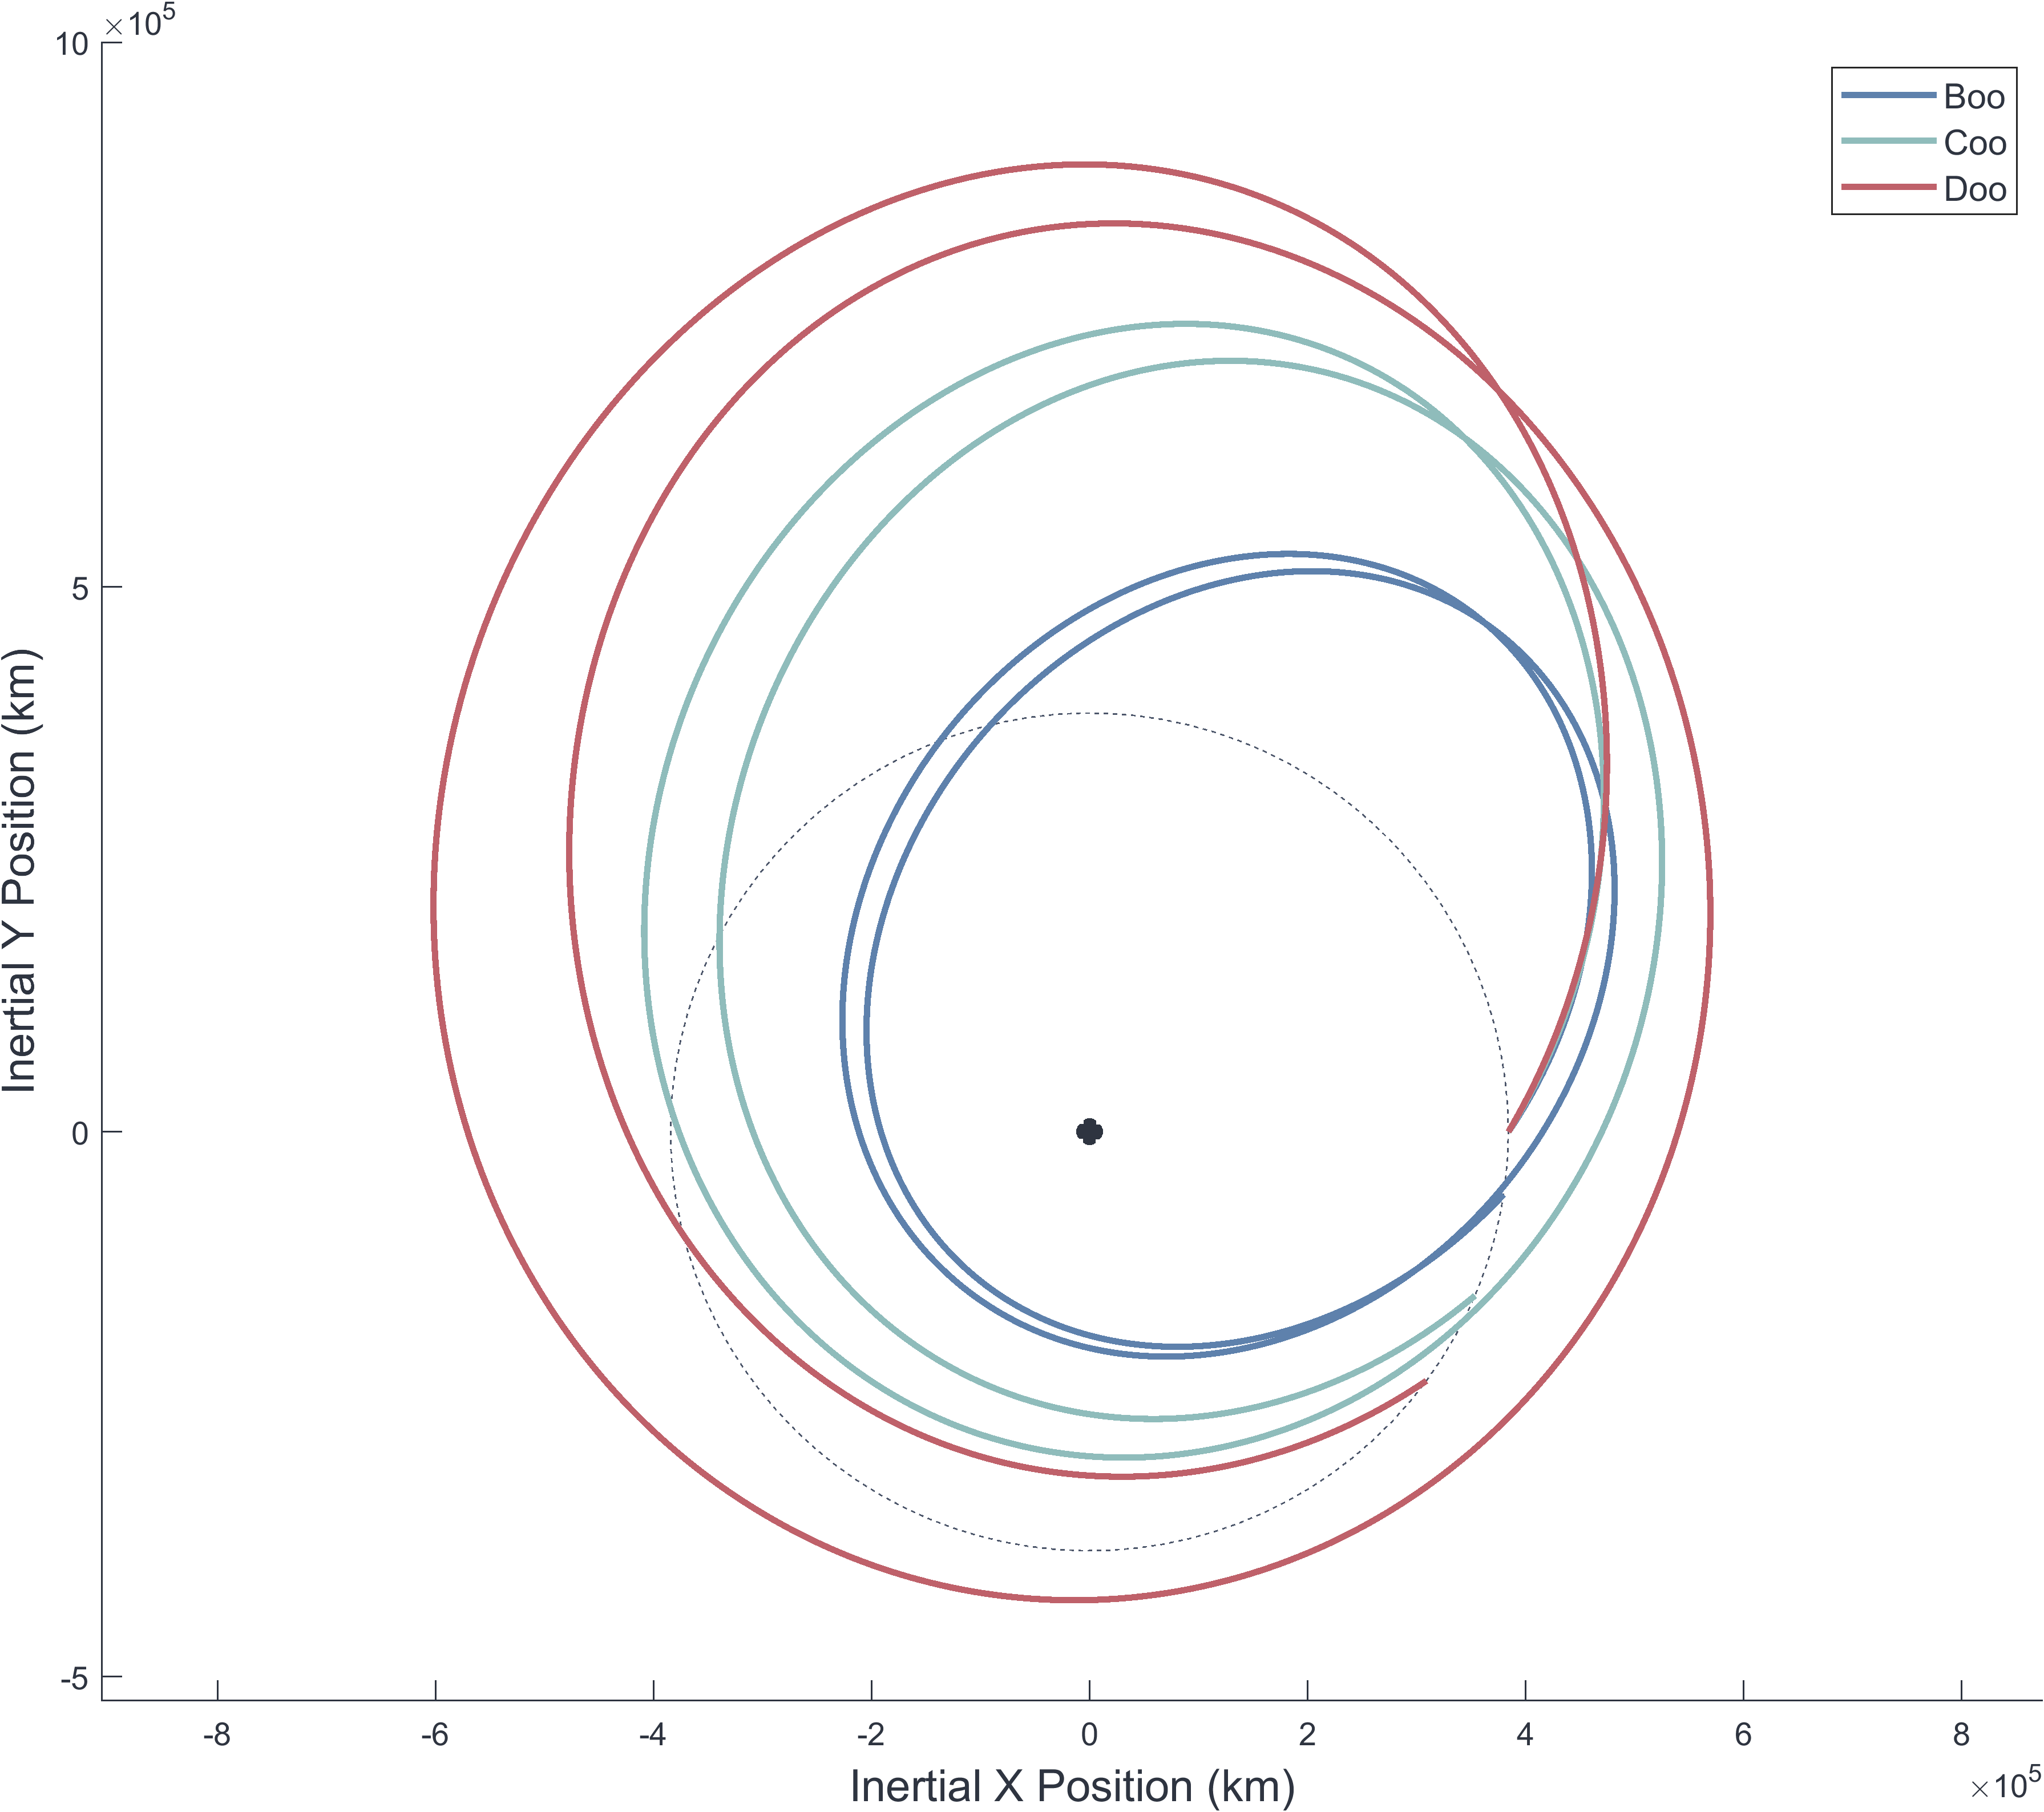
\includegraphics[trim=75 50 0 0, clip, width=3in]{./figs/mooni_FamilyPlot_oo_vInf0.6_theta60.png}
        % \caption{Top 12 results from Galileo dataset, color sorted by sequence}
    \end{subfigure}
\end{figure}
\begin{figure}[h]
    \centering
    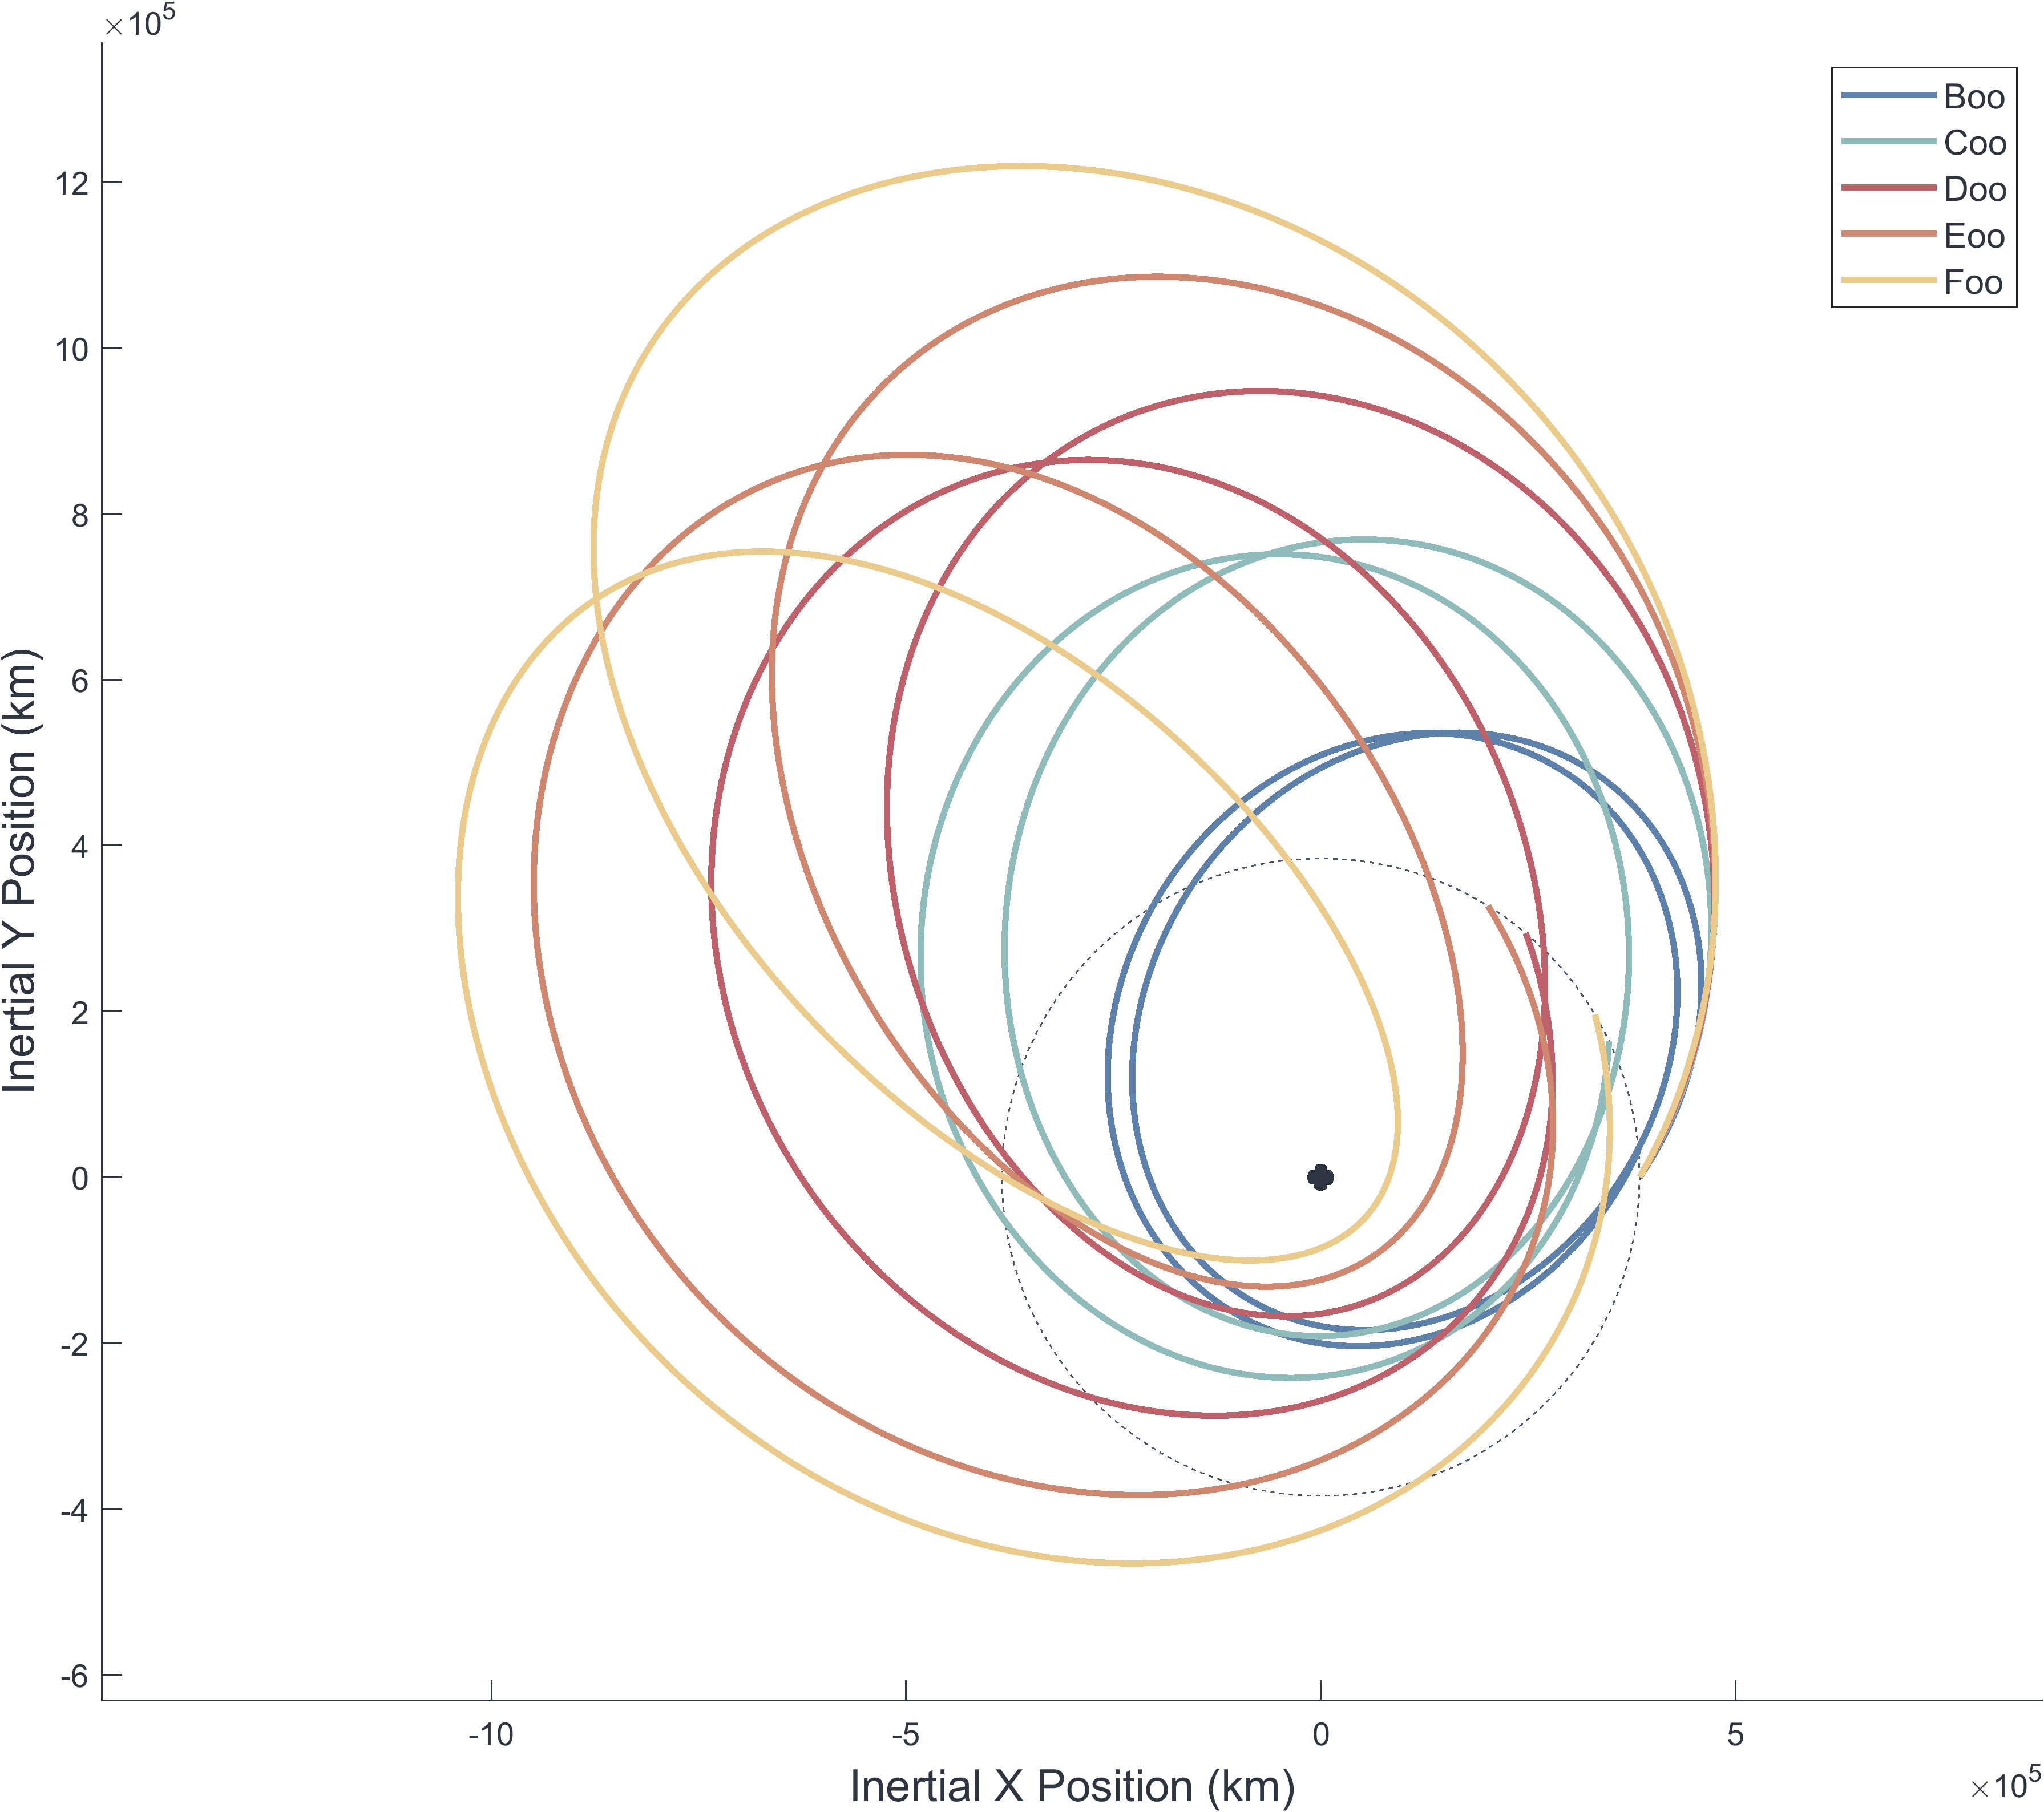
\includegraphics[trim=75 50 0 0, clip, width=3in]{./figs/mooni_FamilyPlot_oo_vInf0.6_theta120.png}
    \caption{Progression of oo family orbits at a v\(_\infty\) of 0.6 \(^{km}/_s\) as time of flight is increased across initial Solar Phase Angles, \(\theta_0\), of 0°, 60°, and 120°. Note that all orbits have their initial positions rotated that they are in line with the x-axis.}
    \label{fig:mooni_famPlot_oo_0.6}
\end{figure}


\begin{figure}[h!]
    \begin{subfigure}{}
        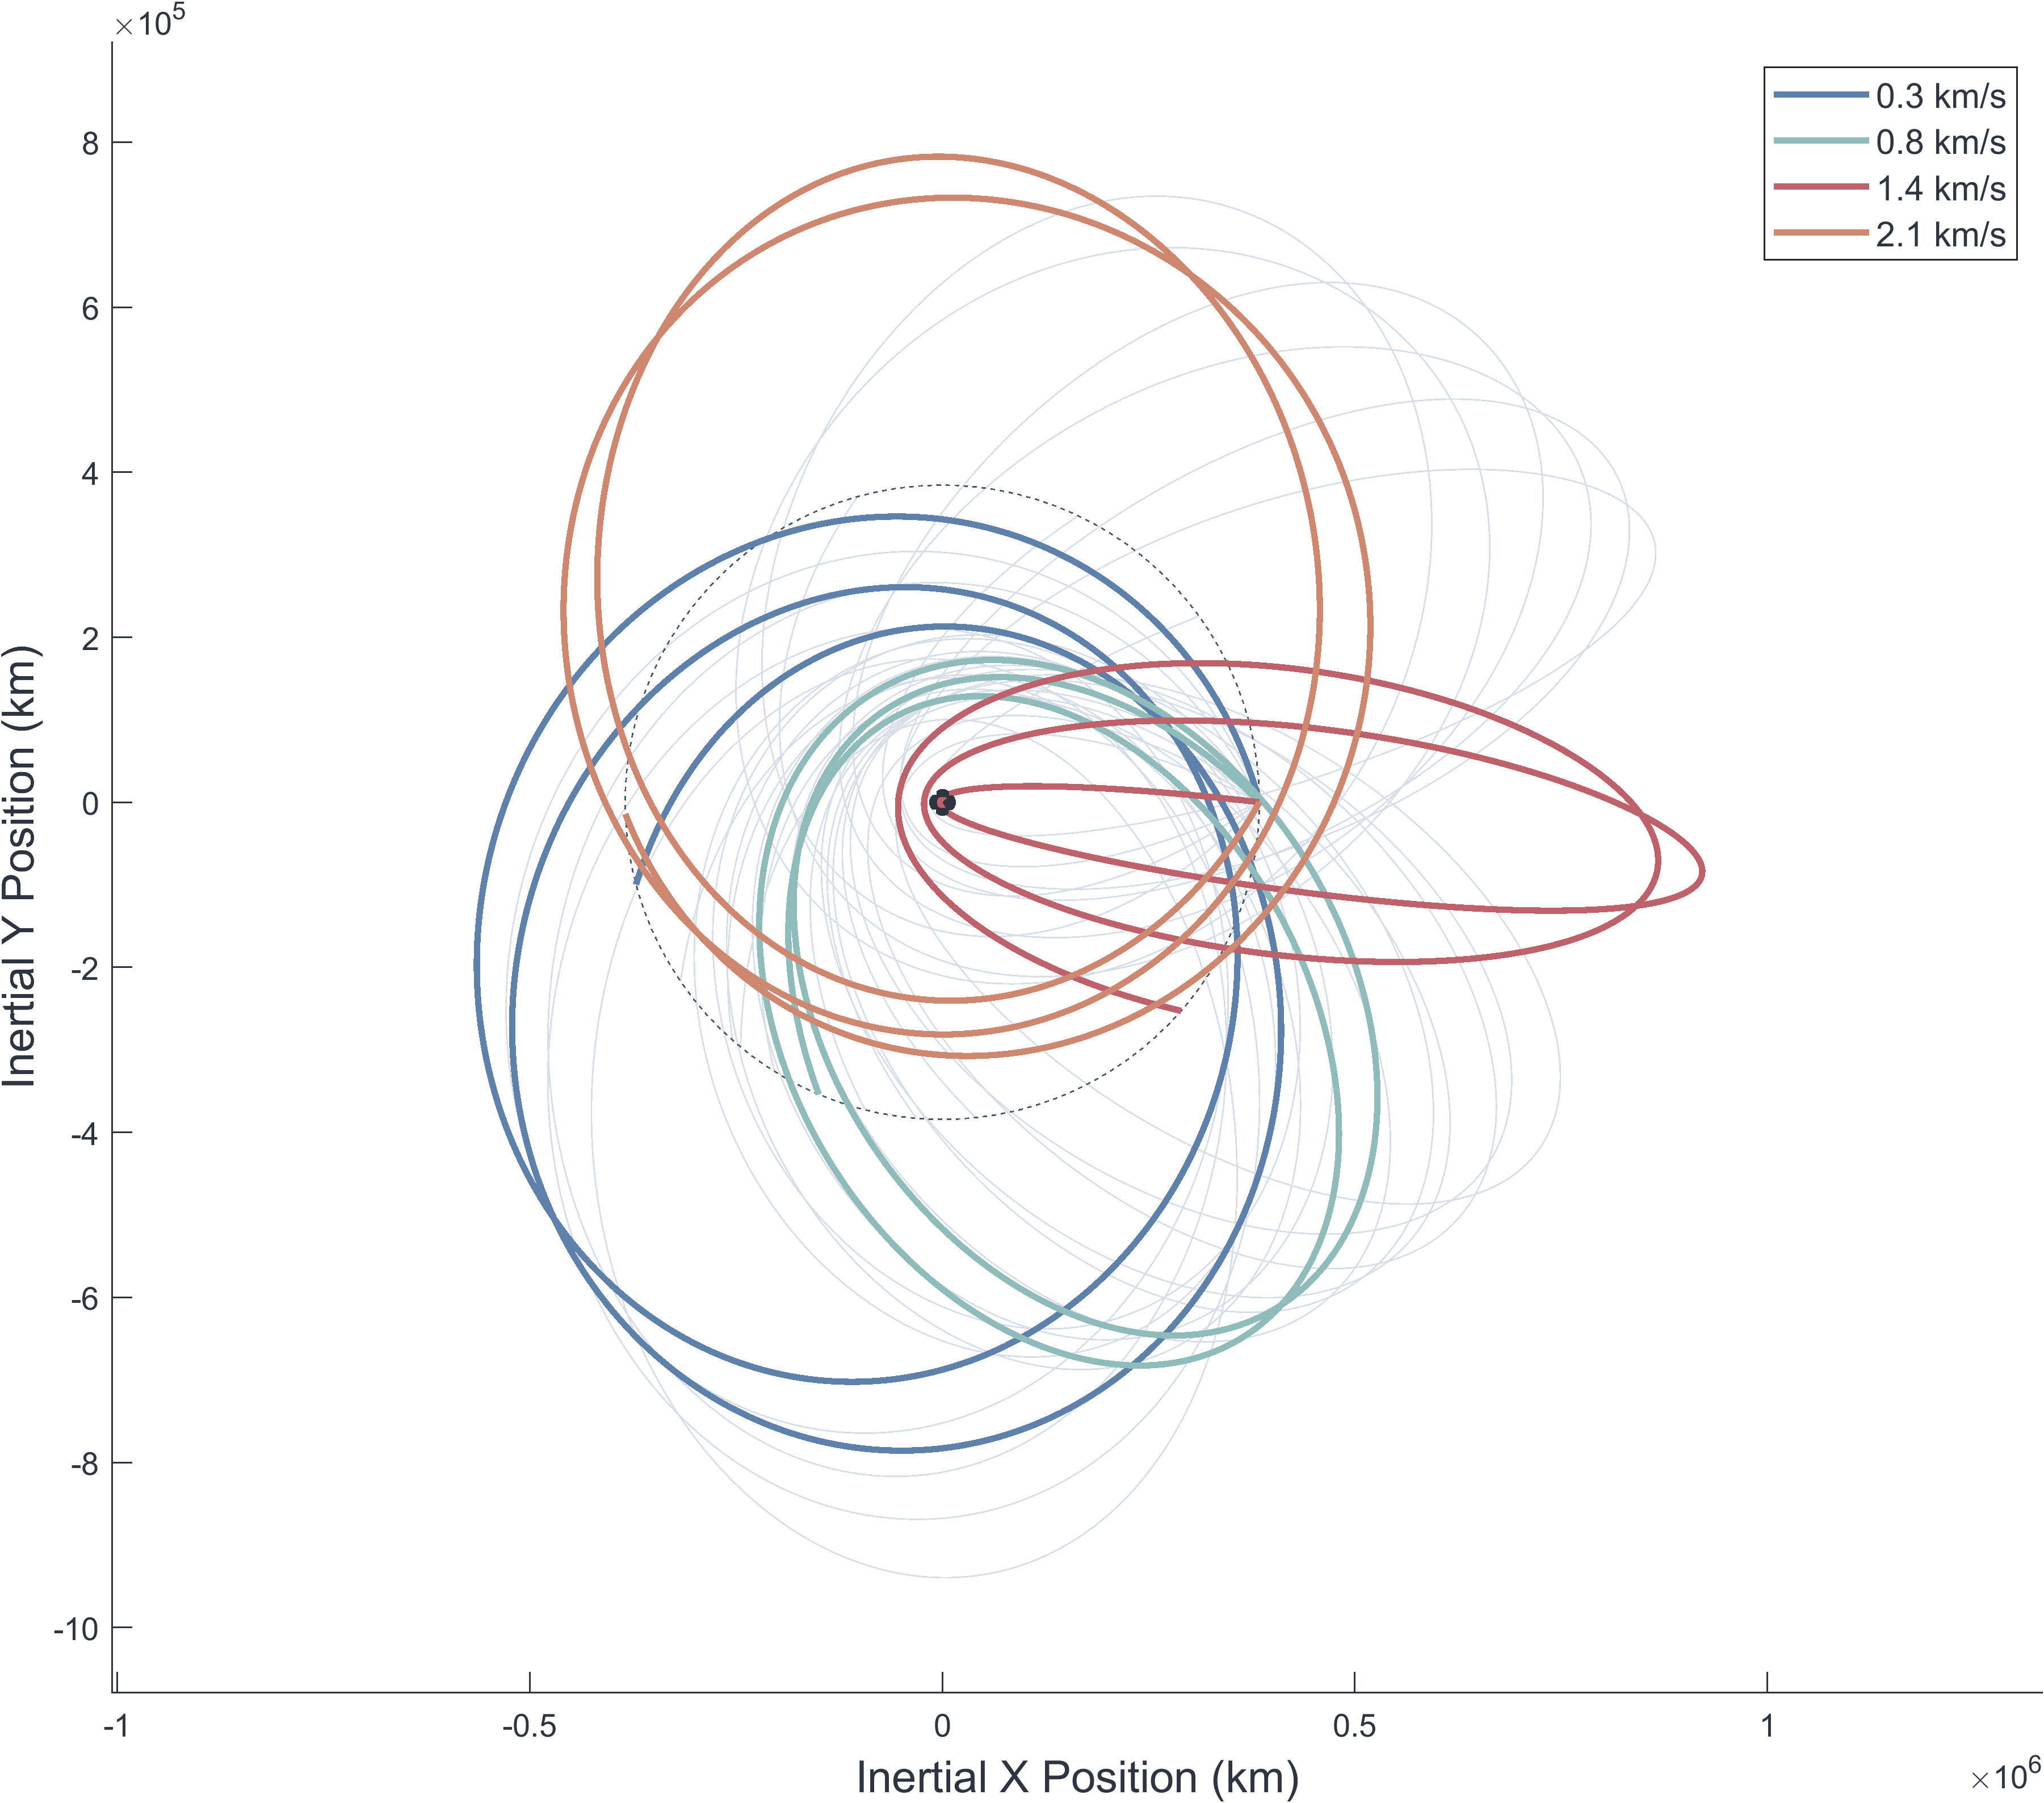
\includegraphics[trim=75 50 0 0, clip, width=3in]{./figs/mooni_vInfPlot_io_famC_theta0.png}
        % \caption{Top 25 results from Europa Clipper dataset, color sorted by sequence}
    \end{subfigure}
    \begin{subfigure}{}
        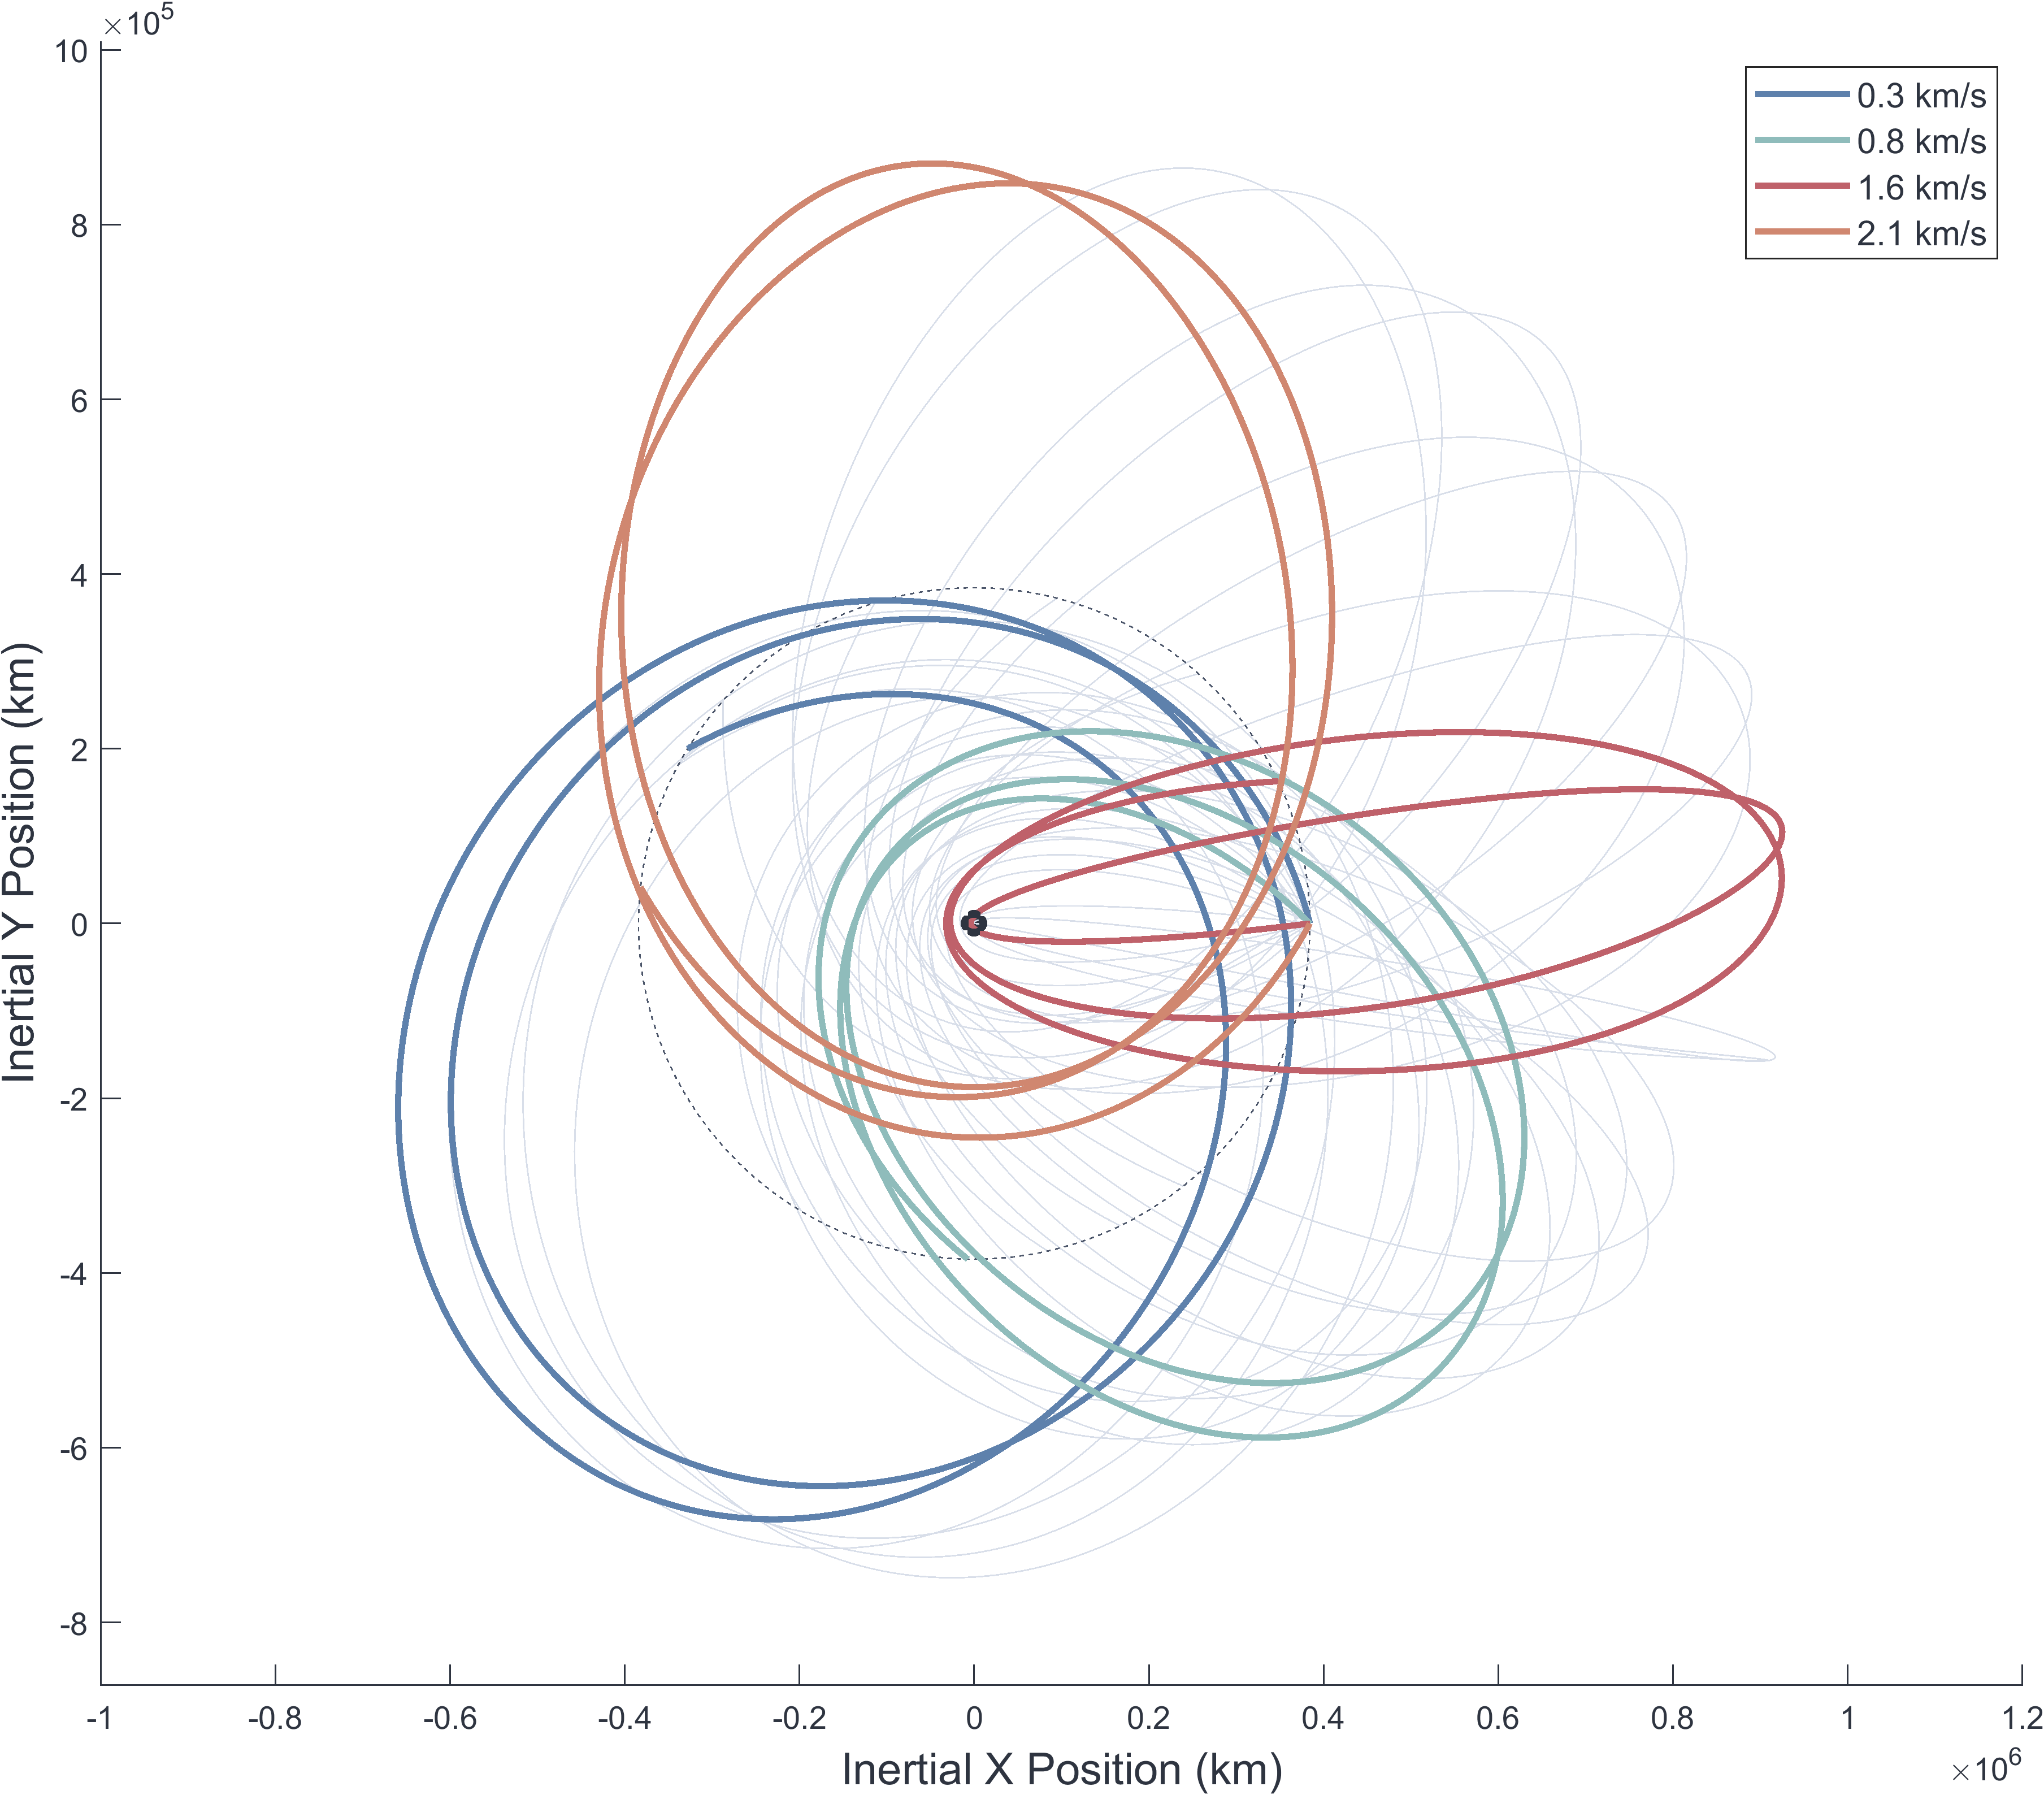
\includegraphics[trim=75 50 0 0, clip, width=3in]{./figs/mooni_vInfPlot_io_famC_theta60.png}
        % \caption{Top 12 results from Galileo dataset, color sorted by sequence}
    \end{subfigure}
\end{figure}
\begin{figure}[h]
    \centering
    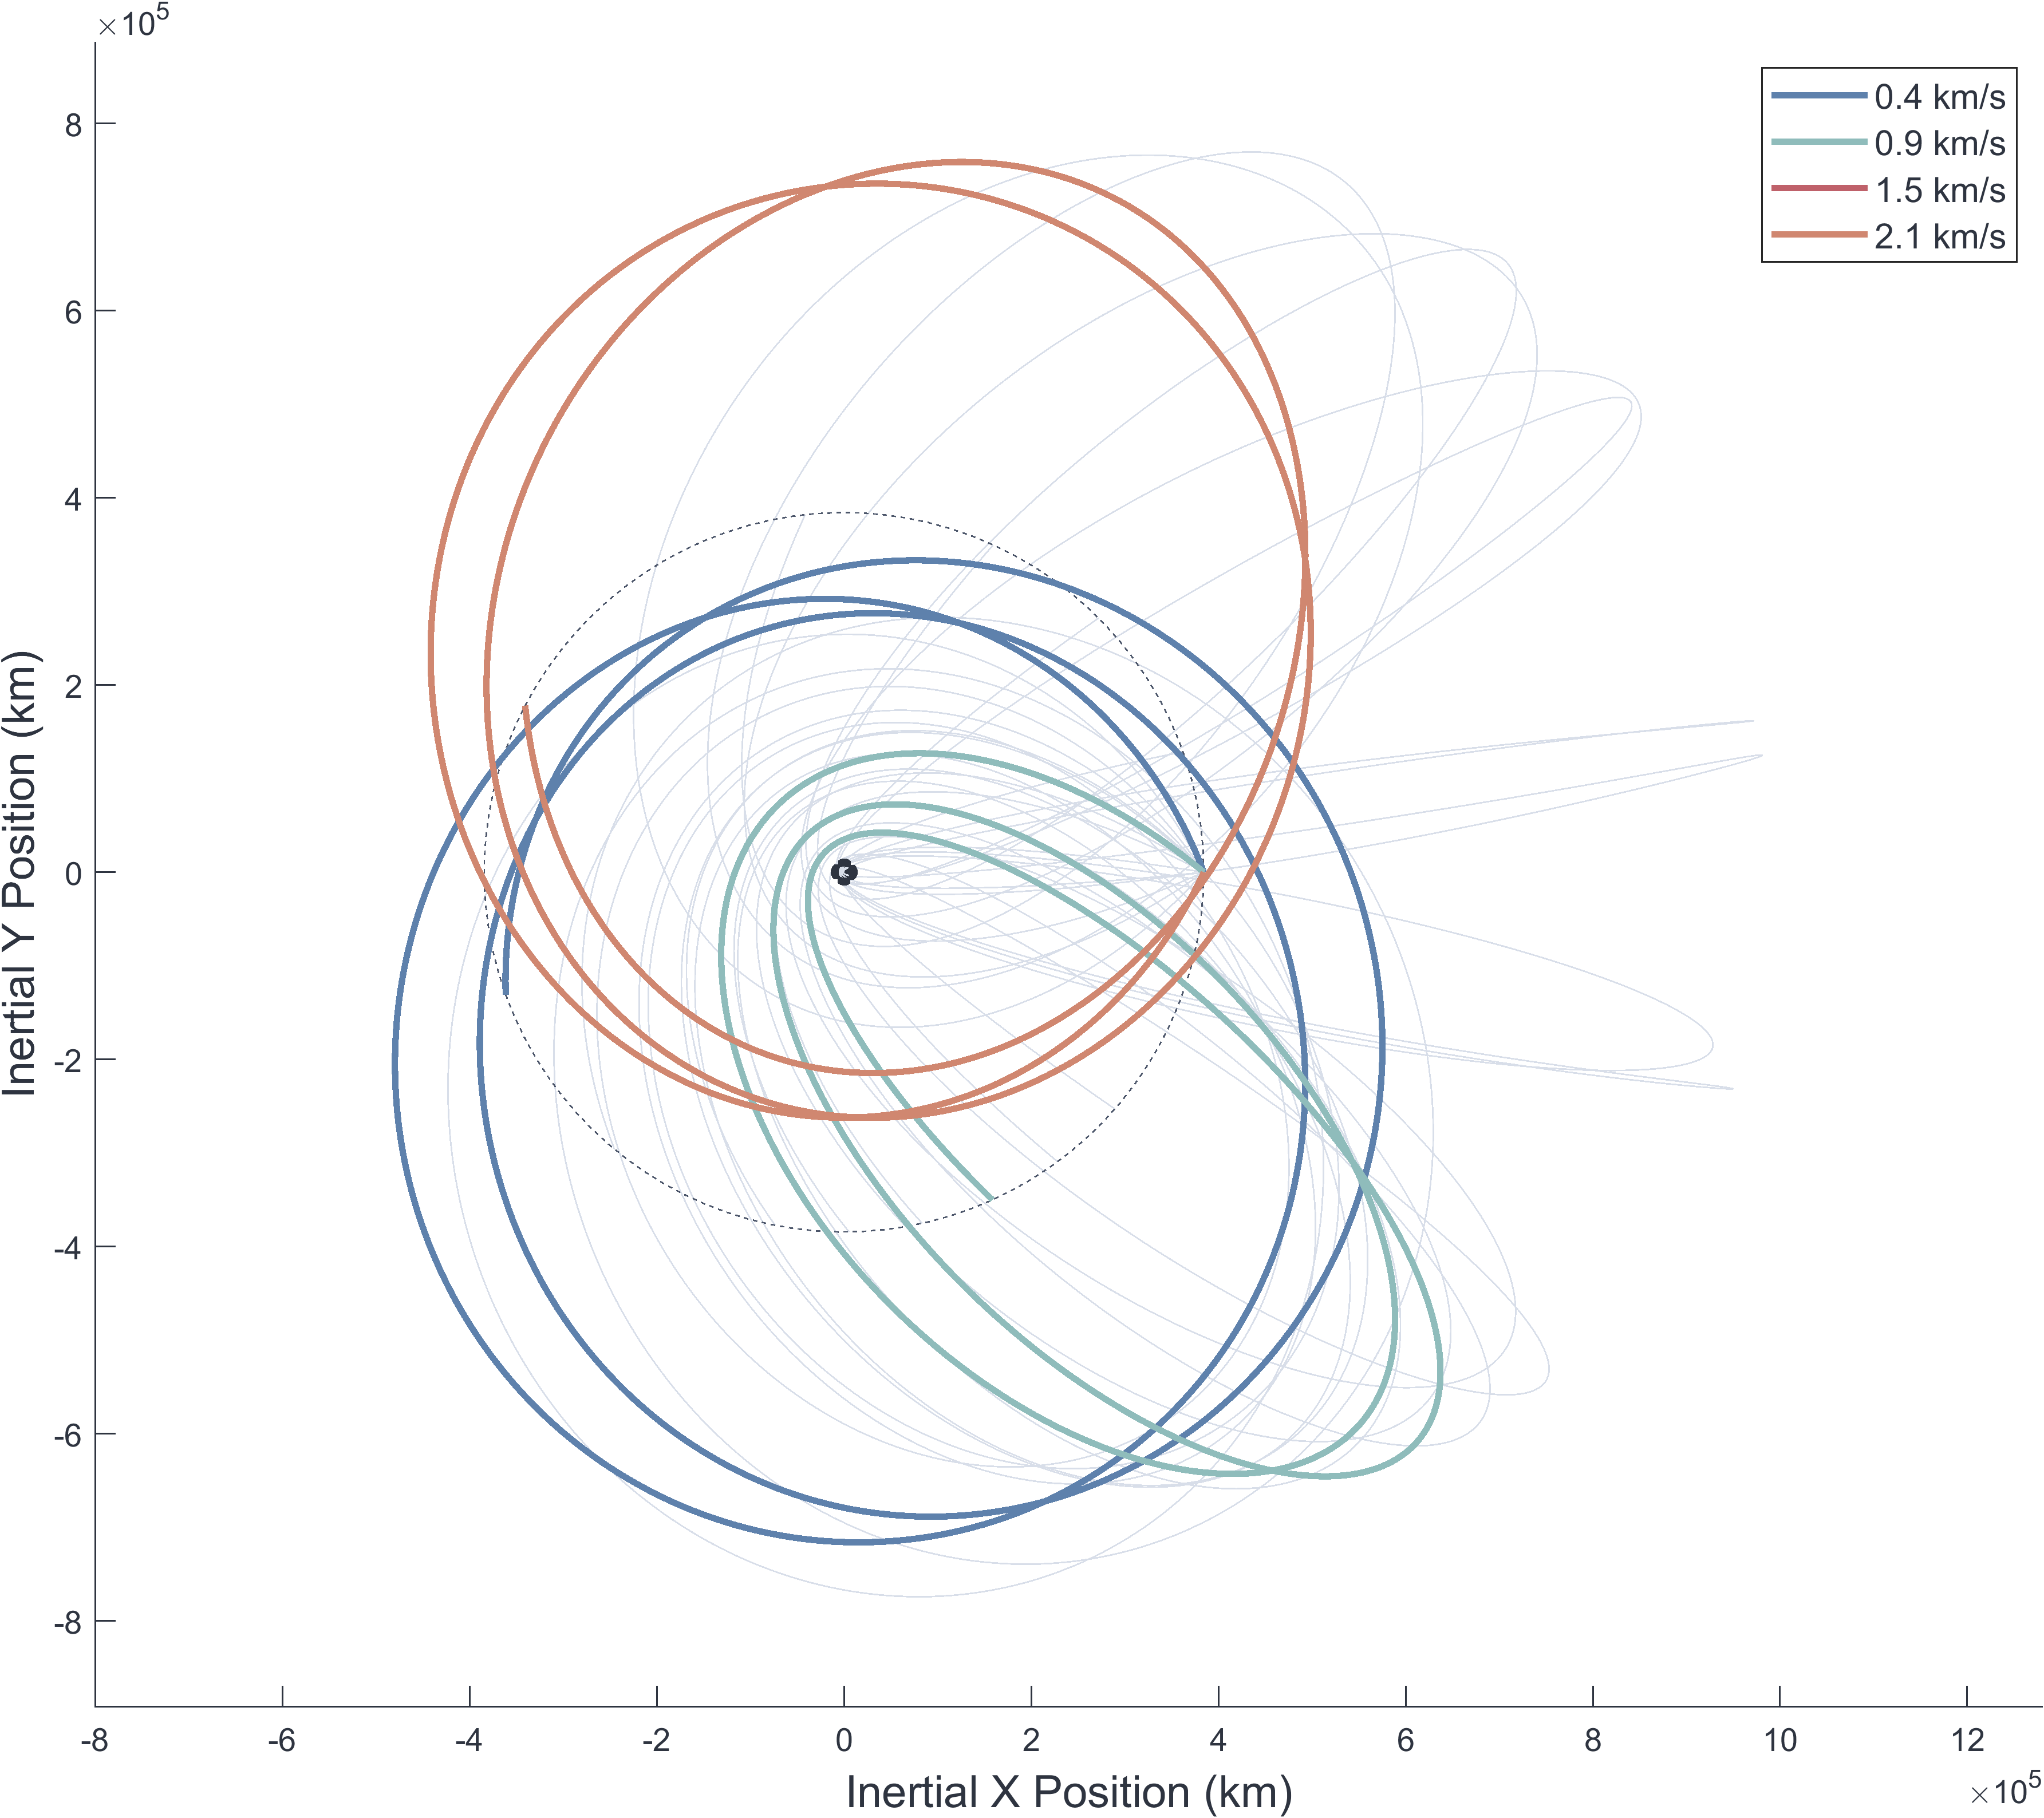
\includegraphics[trim=75 50 0 0, clip, width=3in]{./figs/mooni_vInfPlot_io_famC_theta120.png}
    \caption{Progression of Cio family orbits as v\(_\infty\) is increased across initial Solar Phase Angles, \(\theta_0\), of 0°, 60°, and 120°. As v\(_\infty\) increases, the orbit trends towards an increasingly retrograde starting path from the Moon.}
    \label{fig:mooni_vinfPlot_io_C}
\end{figure}


\begin{figure}[h!]
    \begin{subfigure}{}
        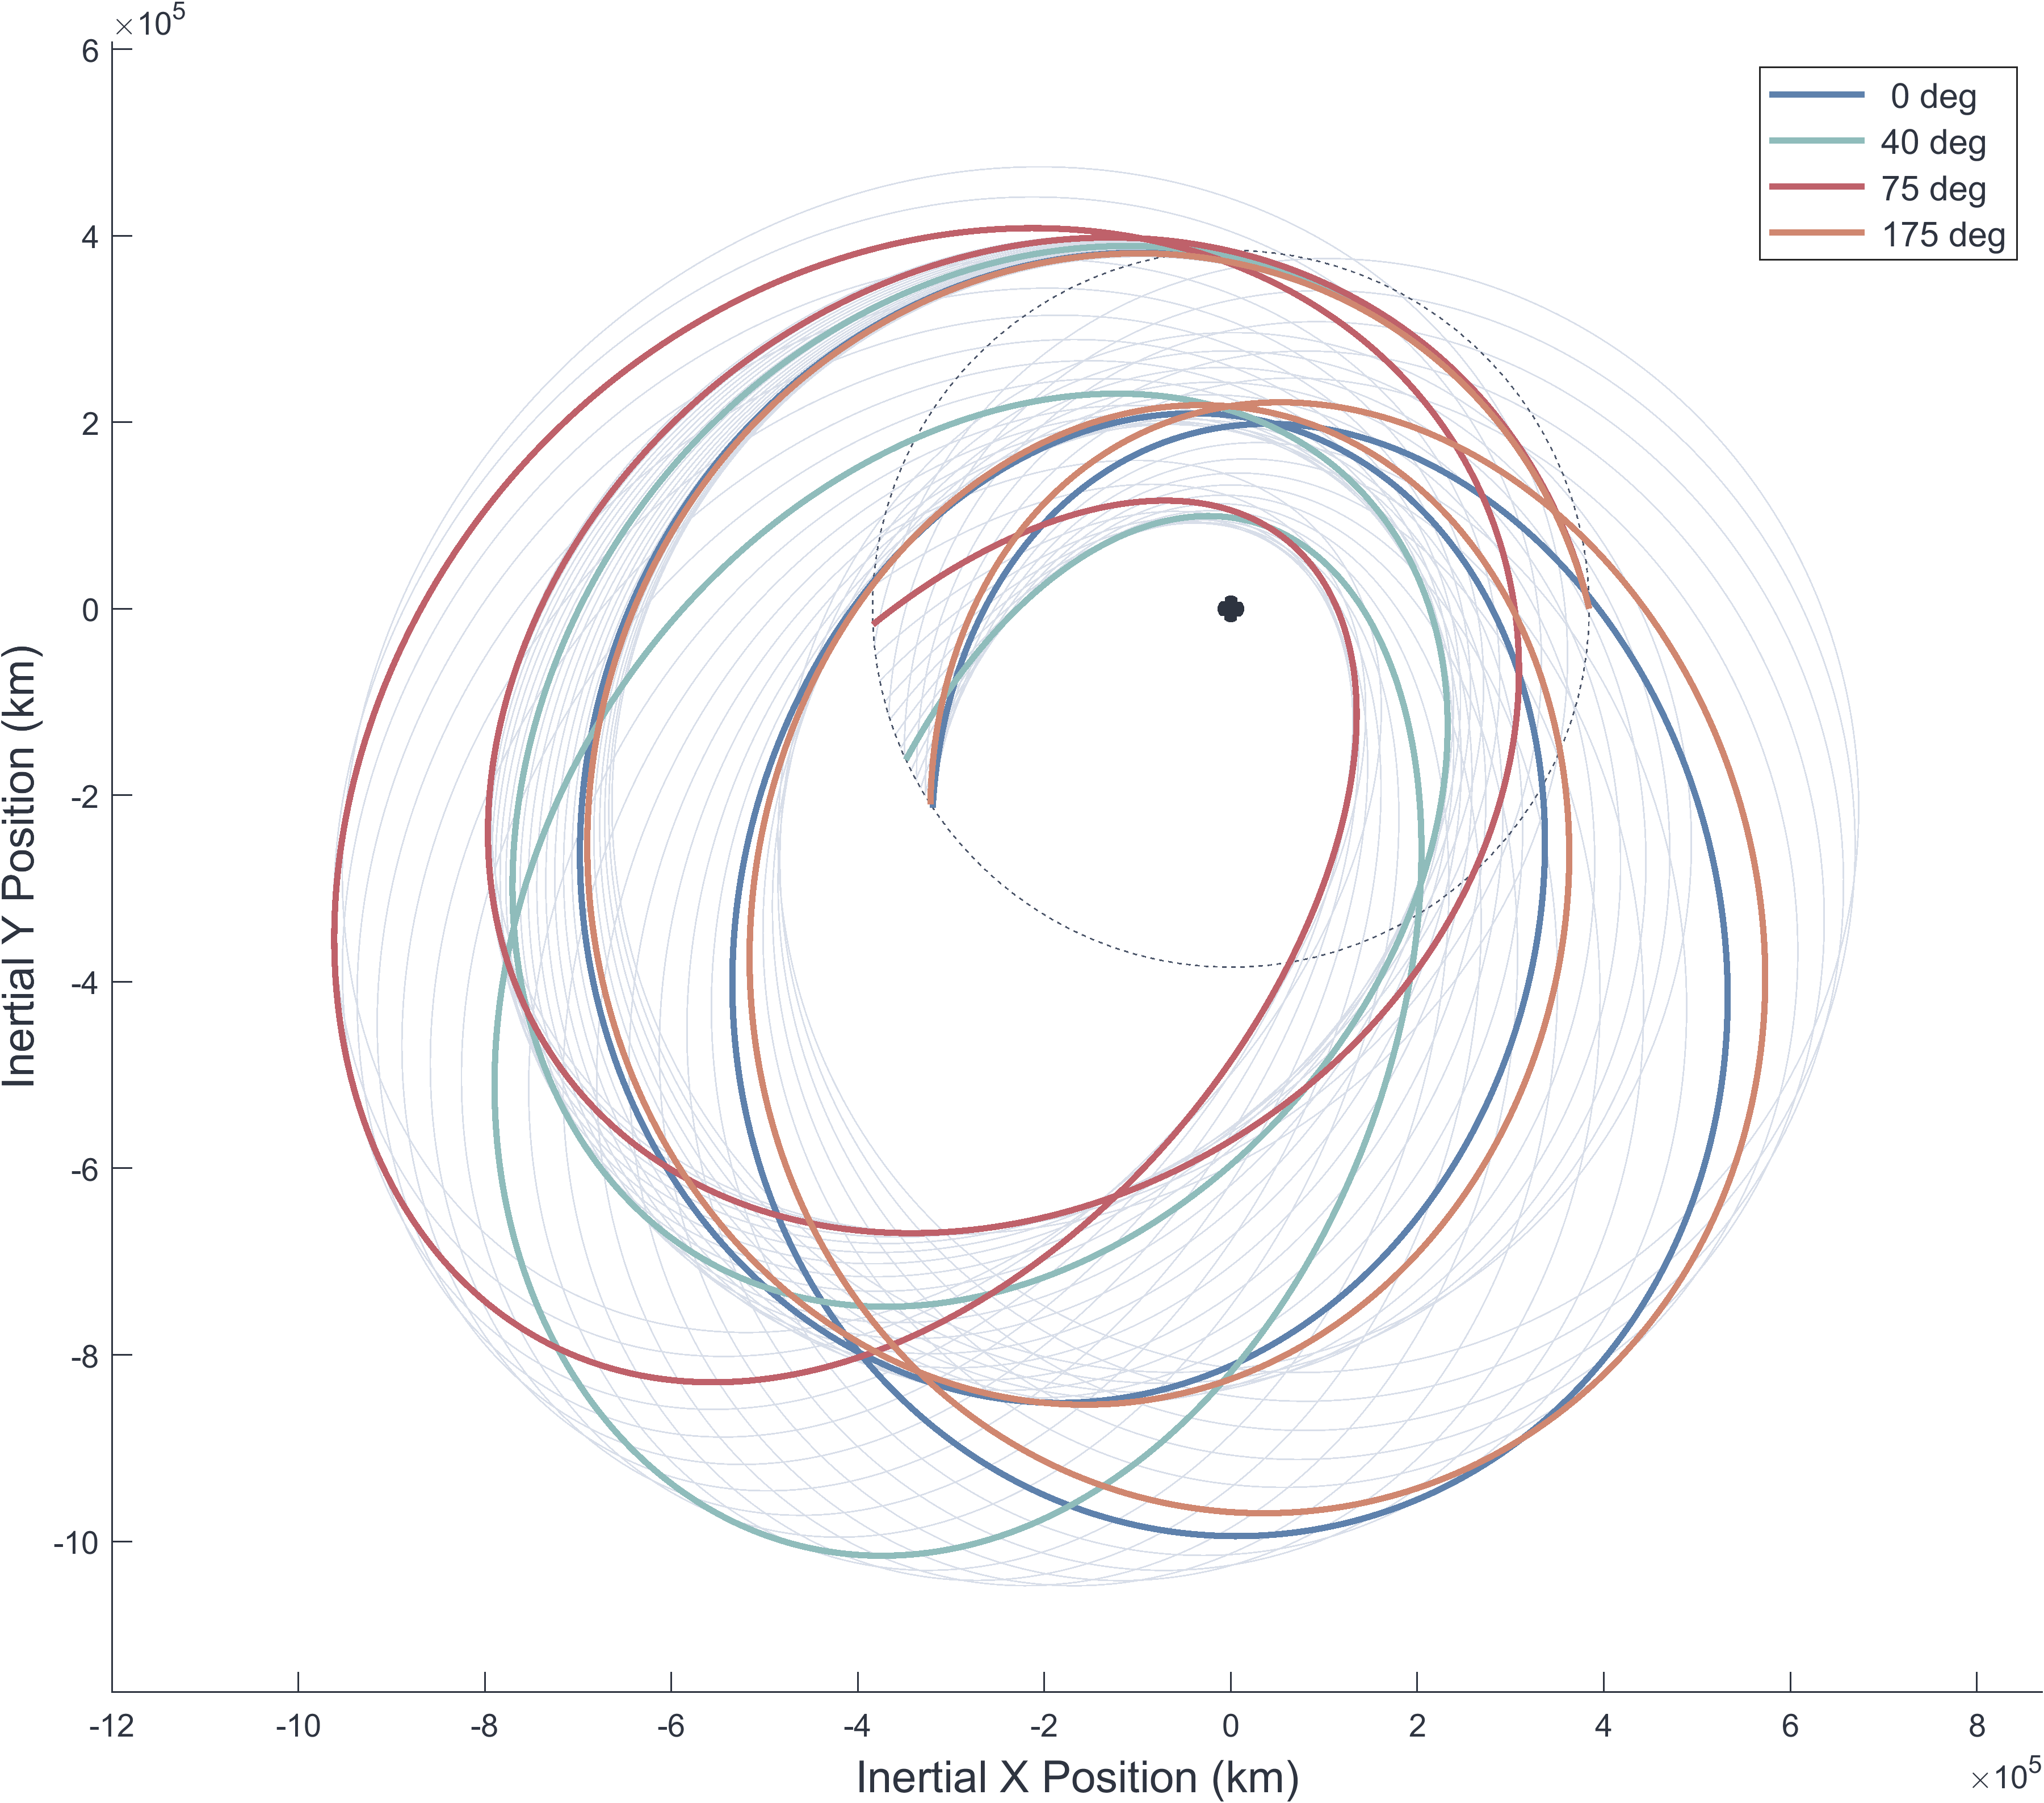
\includegraphics[trim=75 50 0 0, clip, width=2.75in]{./figs/mooni_ThetaPlot_io_famE_vInf0.3.png}
        % \caption{Top 25 results from Europa Clipper dataset, color sorted by sequence}
    \end{subfigure}
    \begin{subfigure}{}
        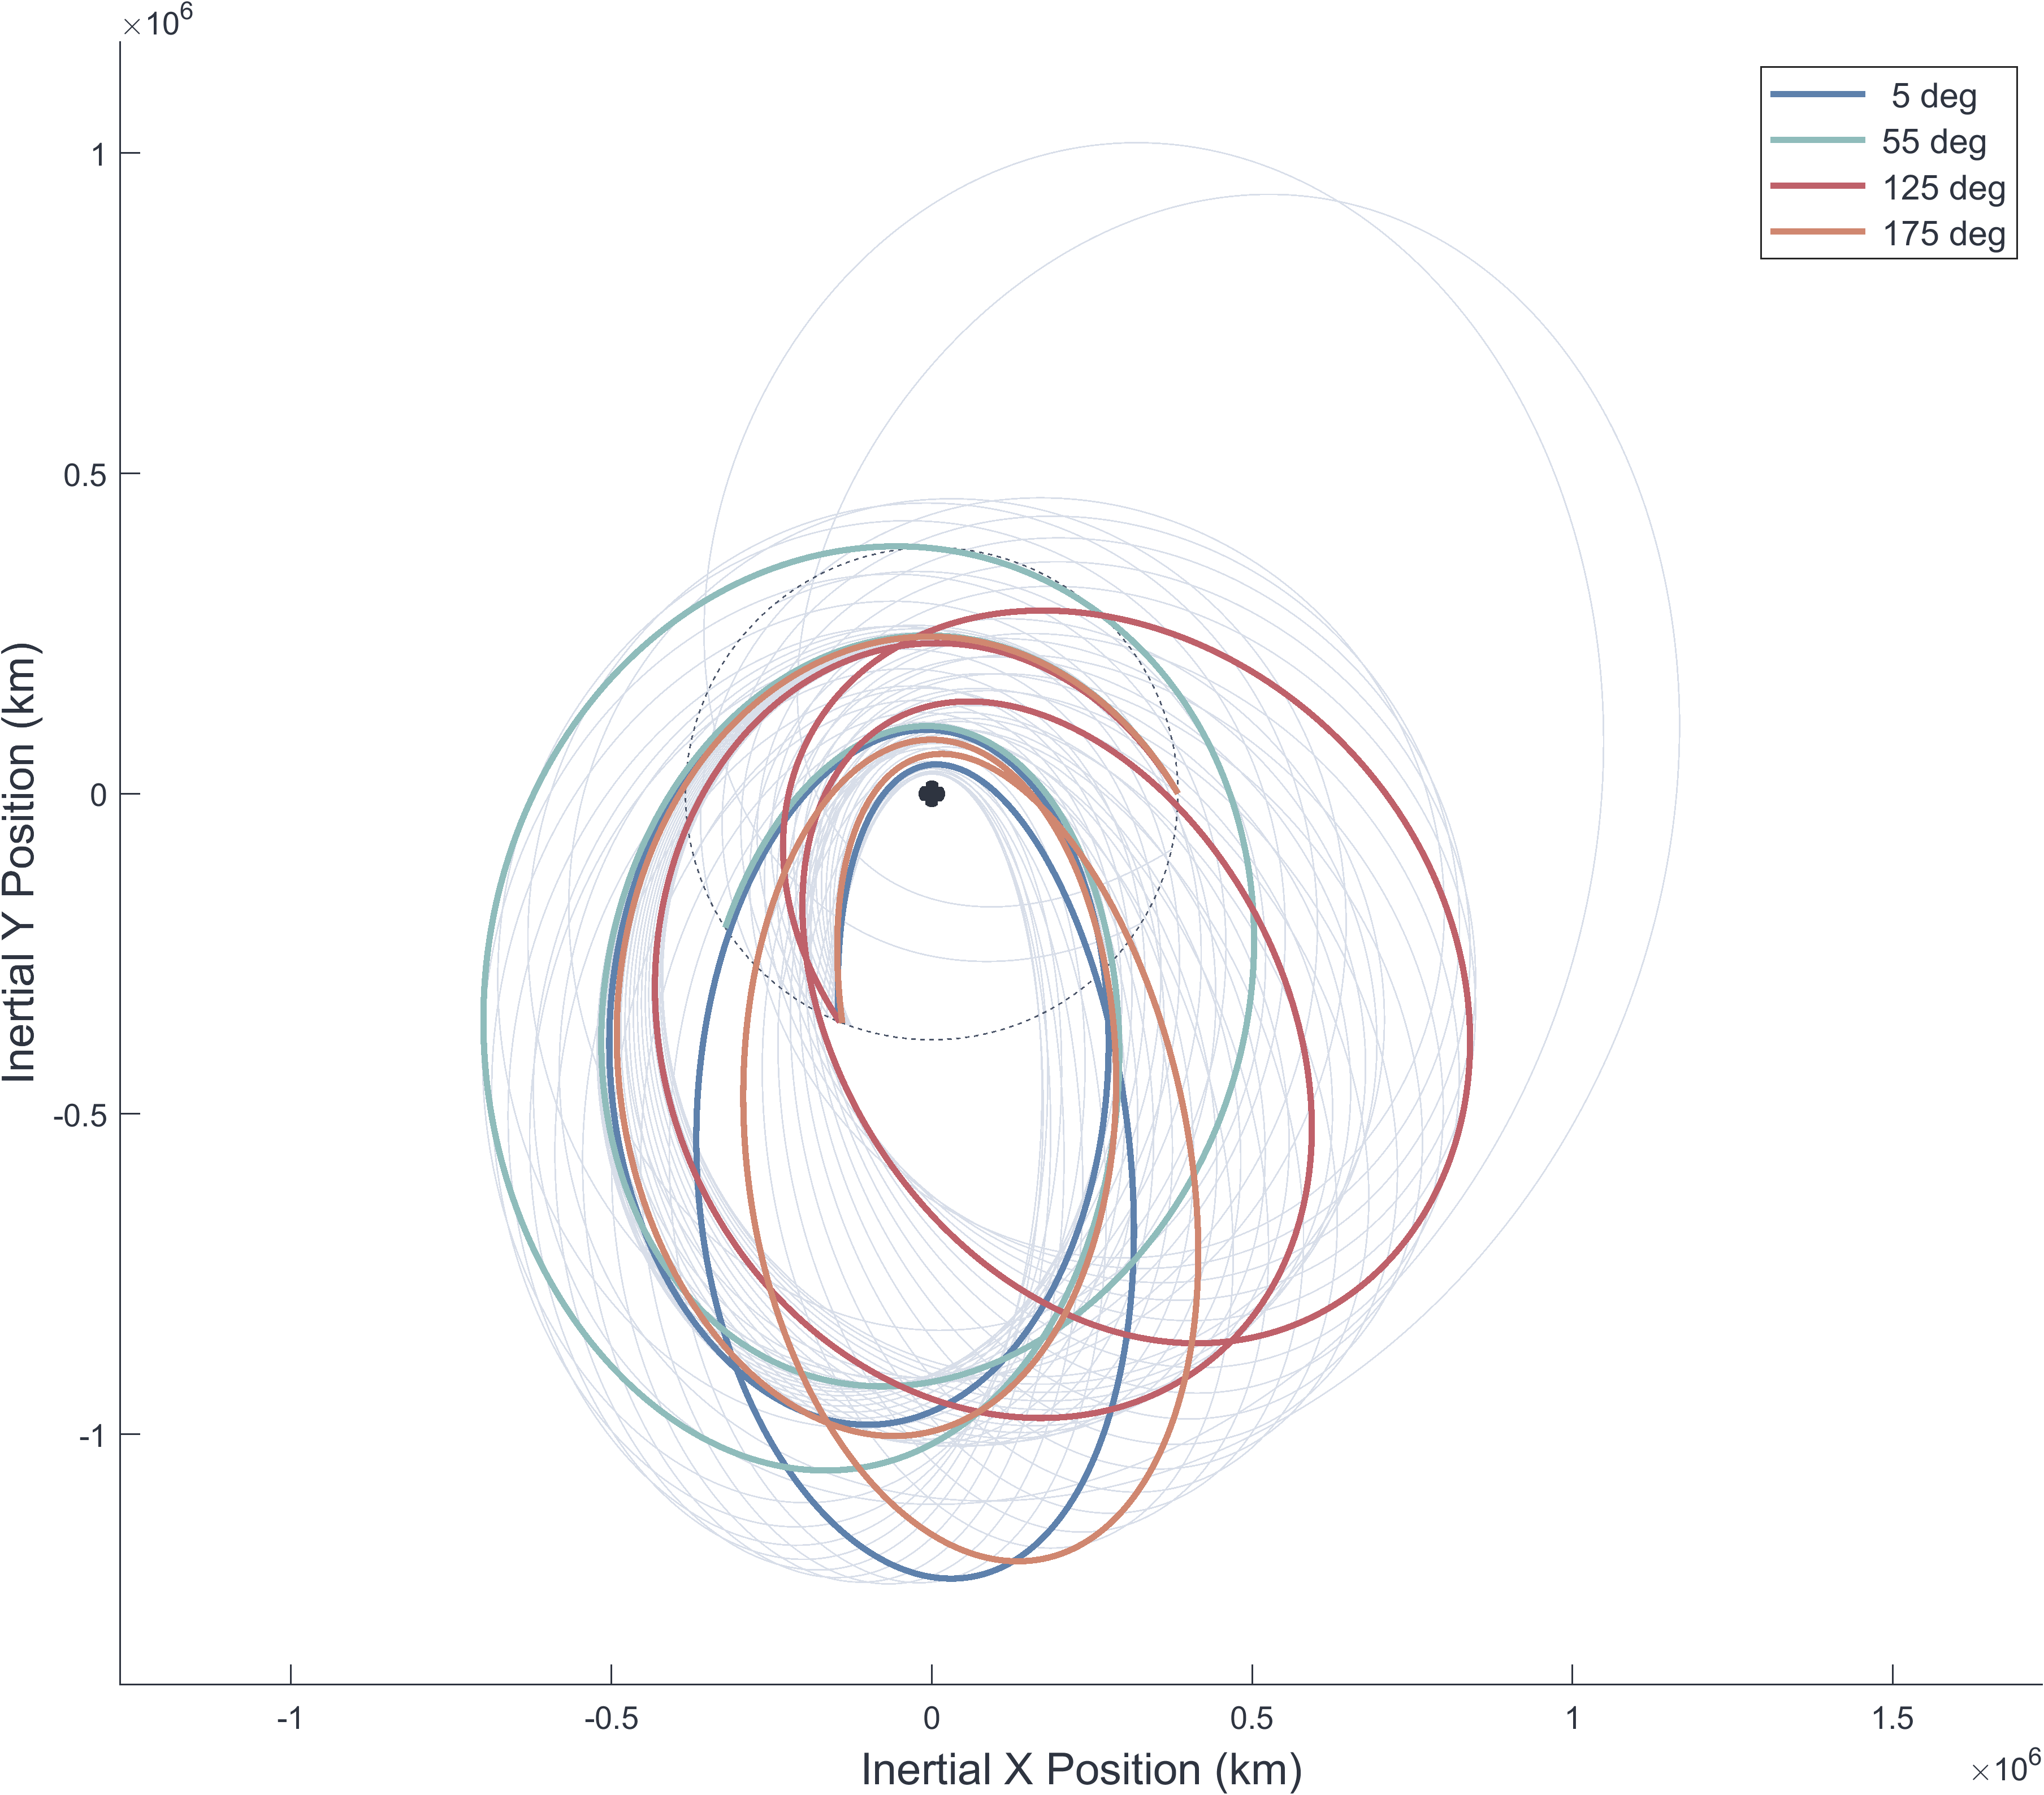
\includegraphics[trim=75 50 0 0, clip, width=2.75in]{./figs/mooni_ThetaPlot_io_famE_vInf0.6.png}
        % \caption{Top 12 results from Galileo dataset, color sorted by sequence}
    \end{subfigure}
\end{figure}
% \vspace{-5cm}z
\begin{figure}[h!]
    \begin{subfigure}{}
        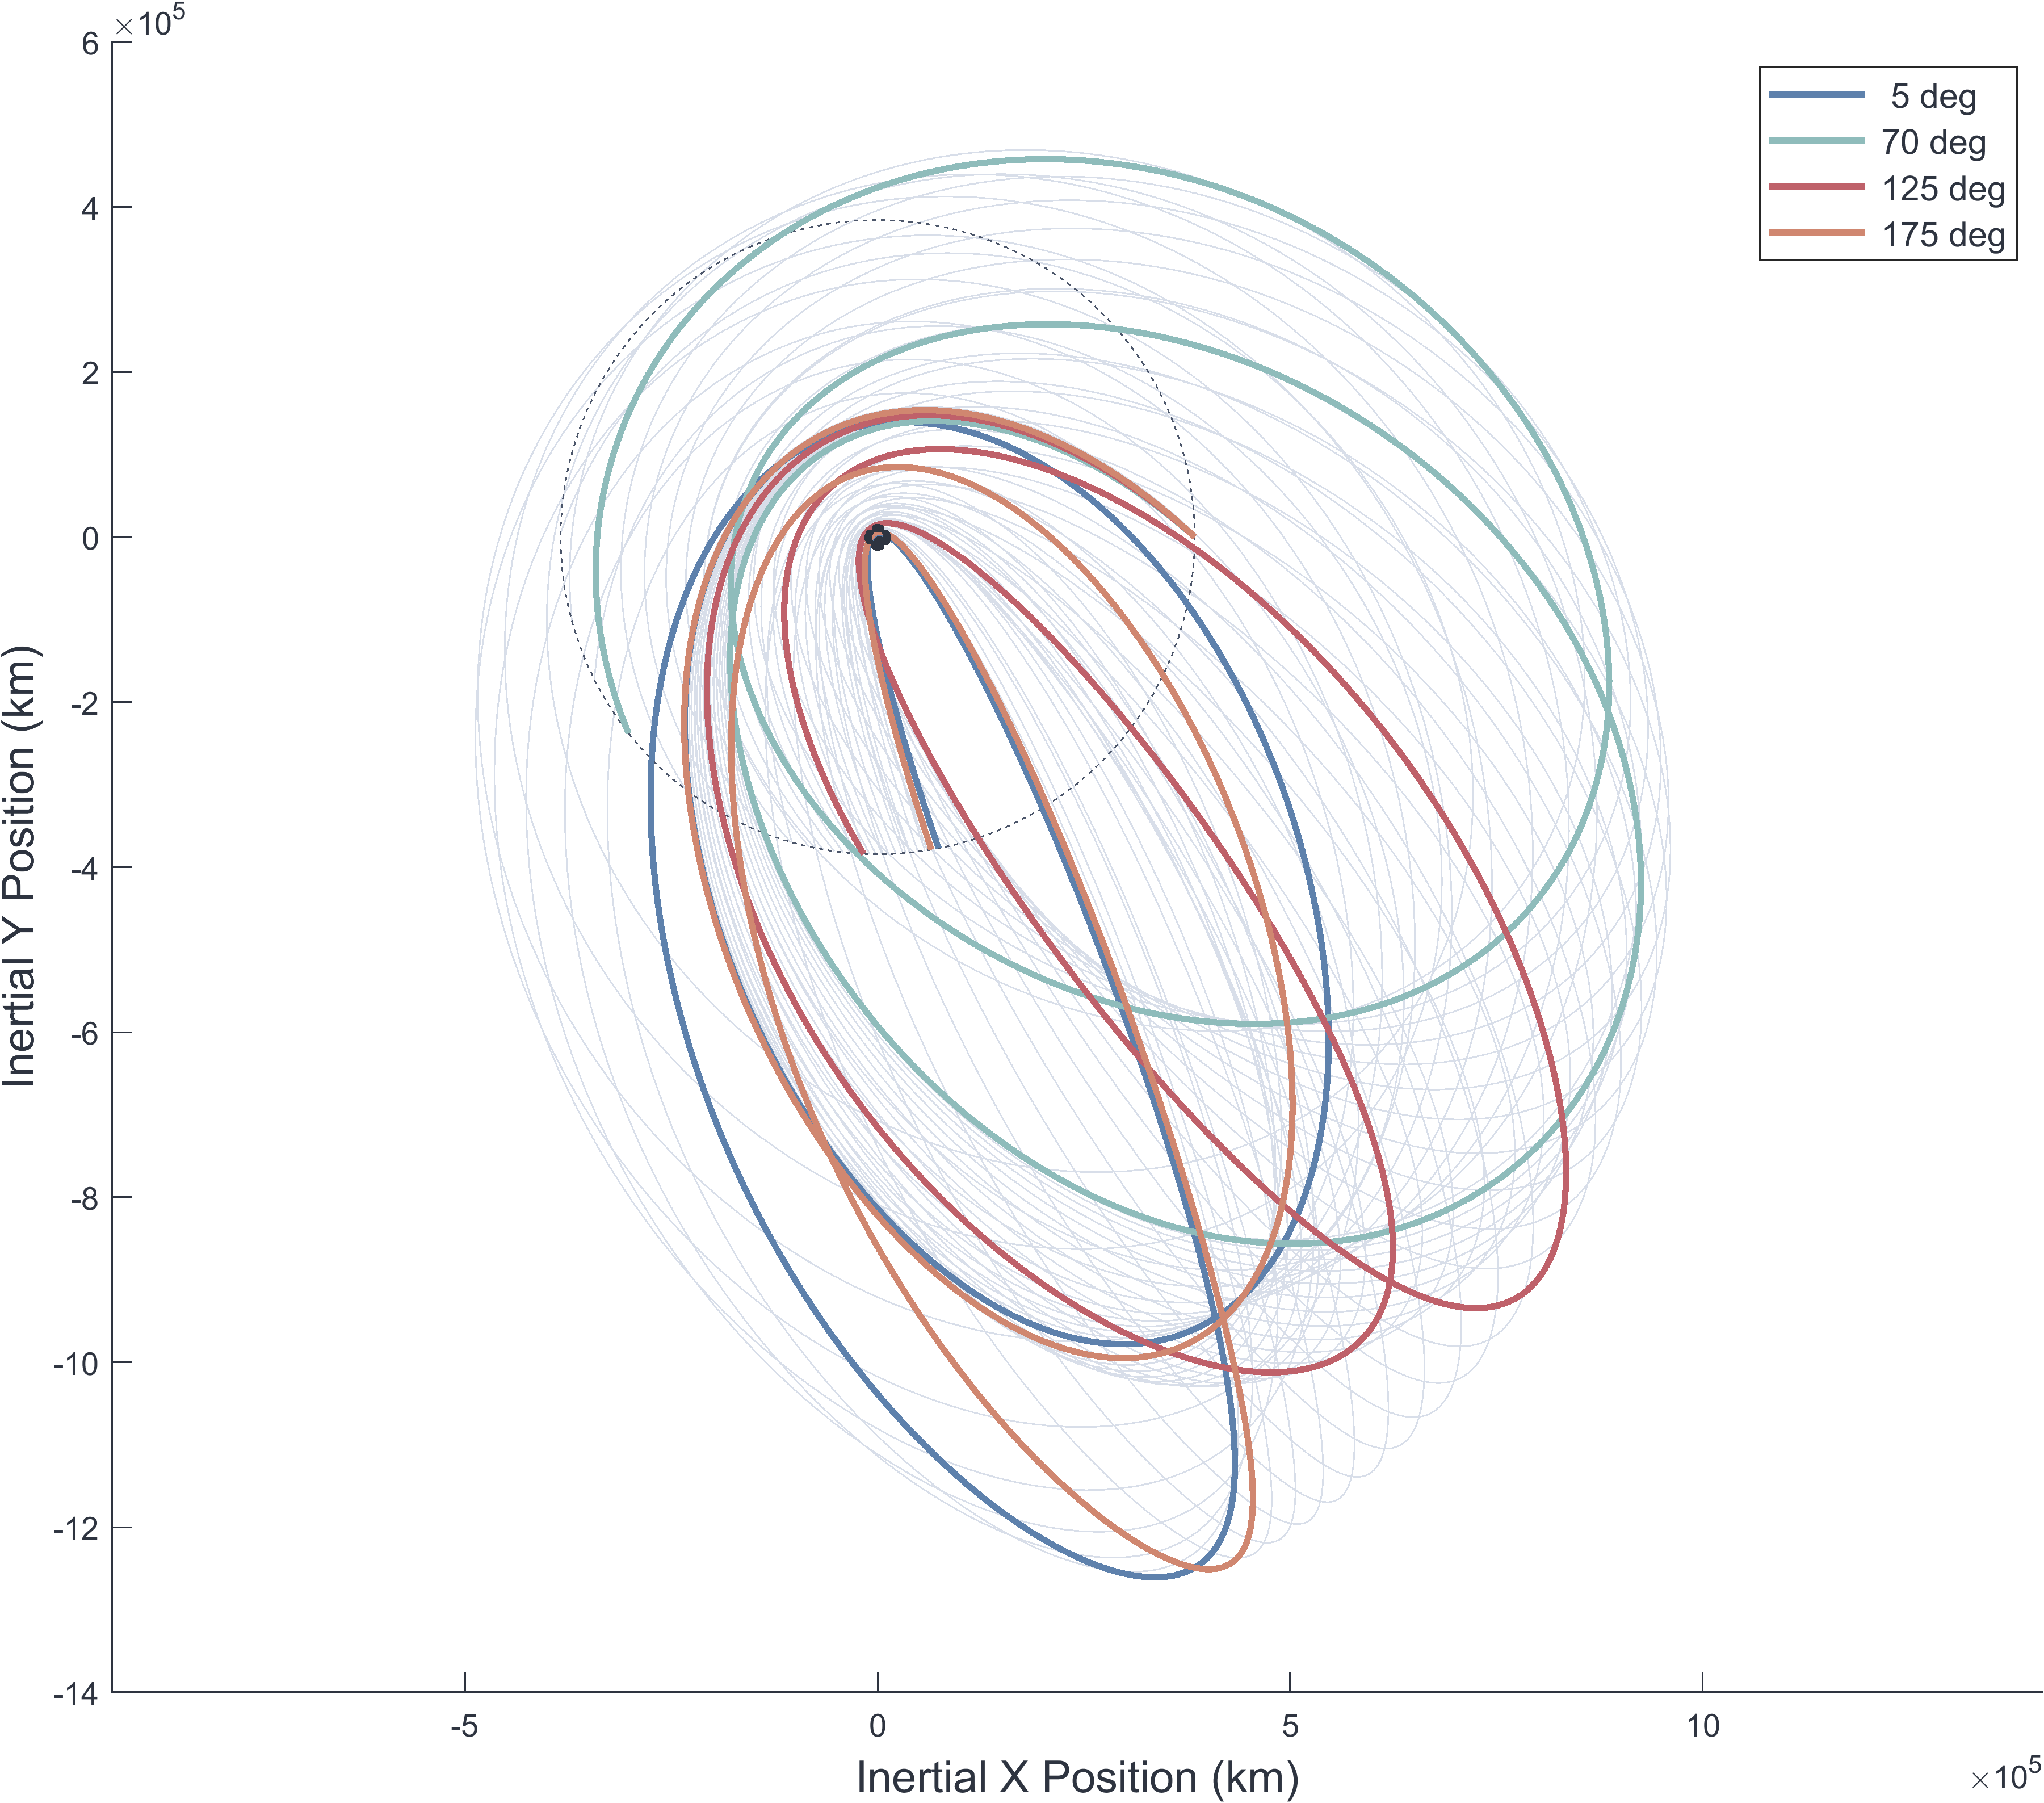
\includegraphics[trim=75 50 0 0, clip, width=2.75in]{./figs/mooni_ThetaPlot_io_famE_vInf0.9.png}
        % \caption{Top 25 results from Europa Clipper dataset, color sorted by sequence}
    \end{subfigure}
    \begin{subfigure}{}
        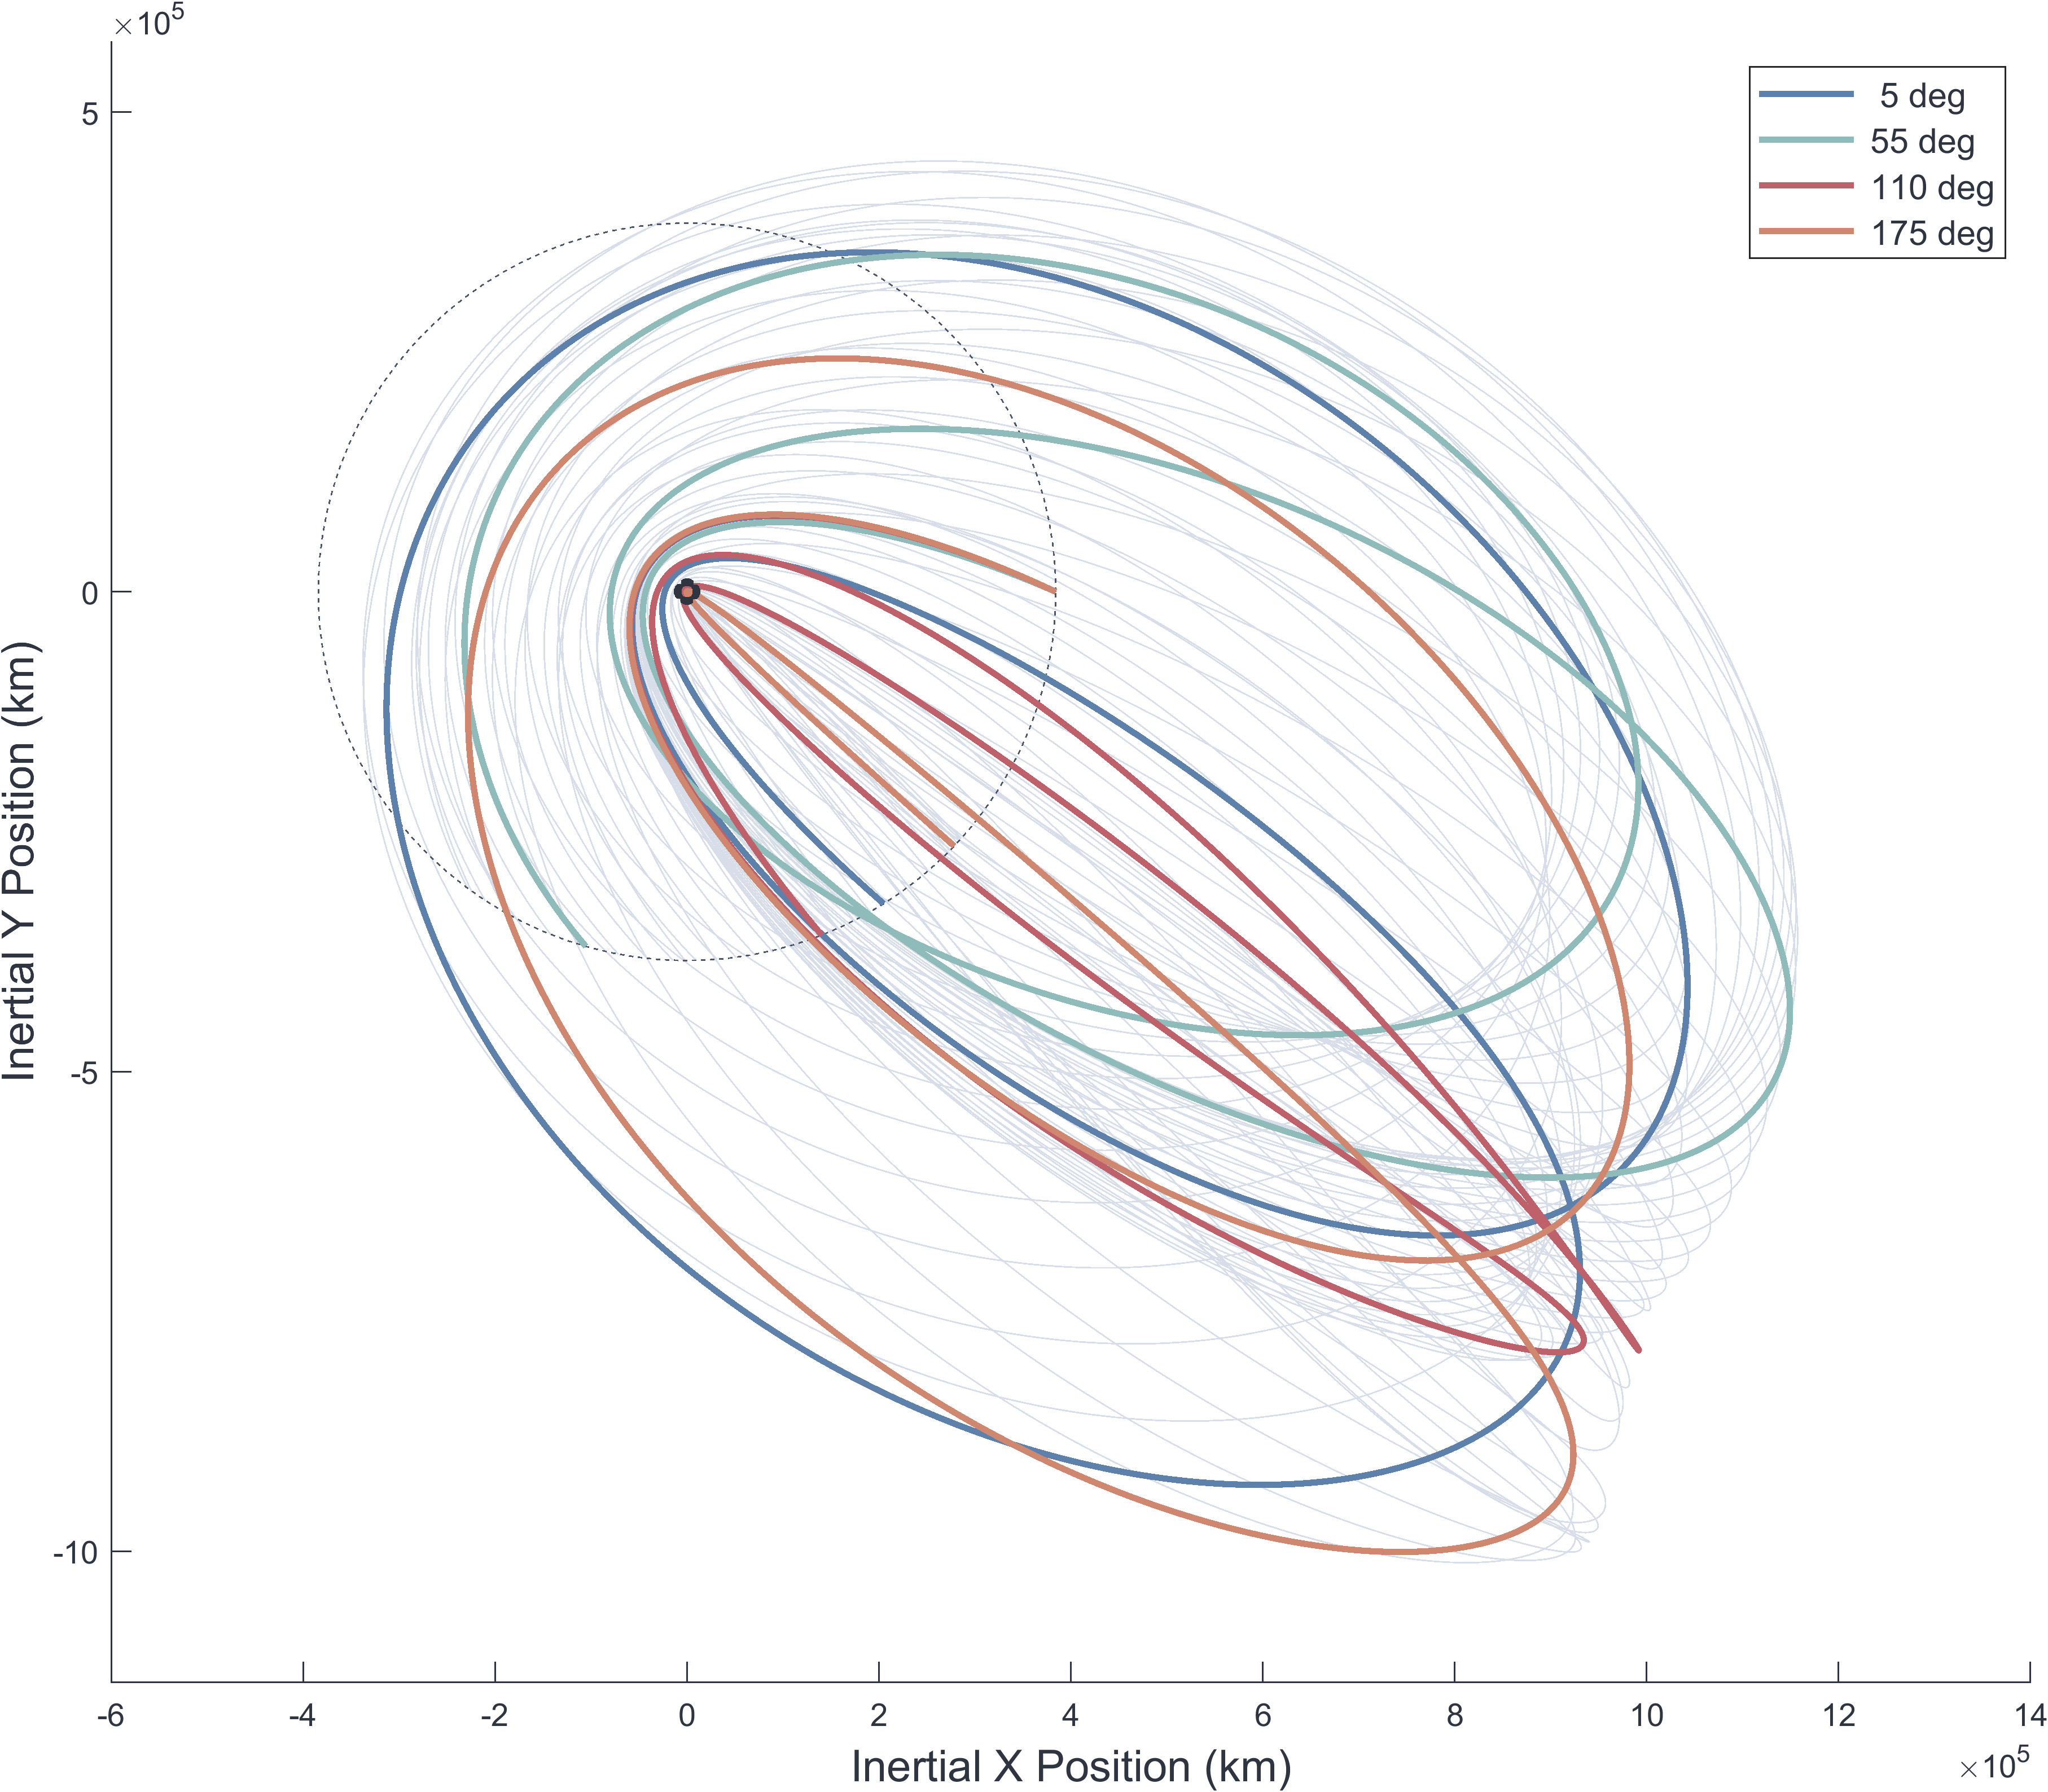
\includegraphics[trim=75 50 0 0, clip, width=2.75in]{./figs/mooni_ThetaPlot_io_famE_vInf1.2.png}
        % \caption{Top 12 results from Galileo dataset, color sorted by sequence}
    \end{subfigure}
\end{figure}
% \vspace{-5cm}
\begin{figure}[h!]
    \begin{subfigure}{}
        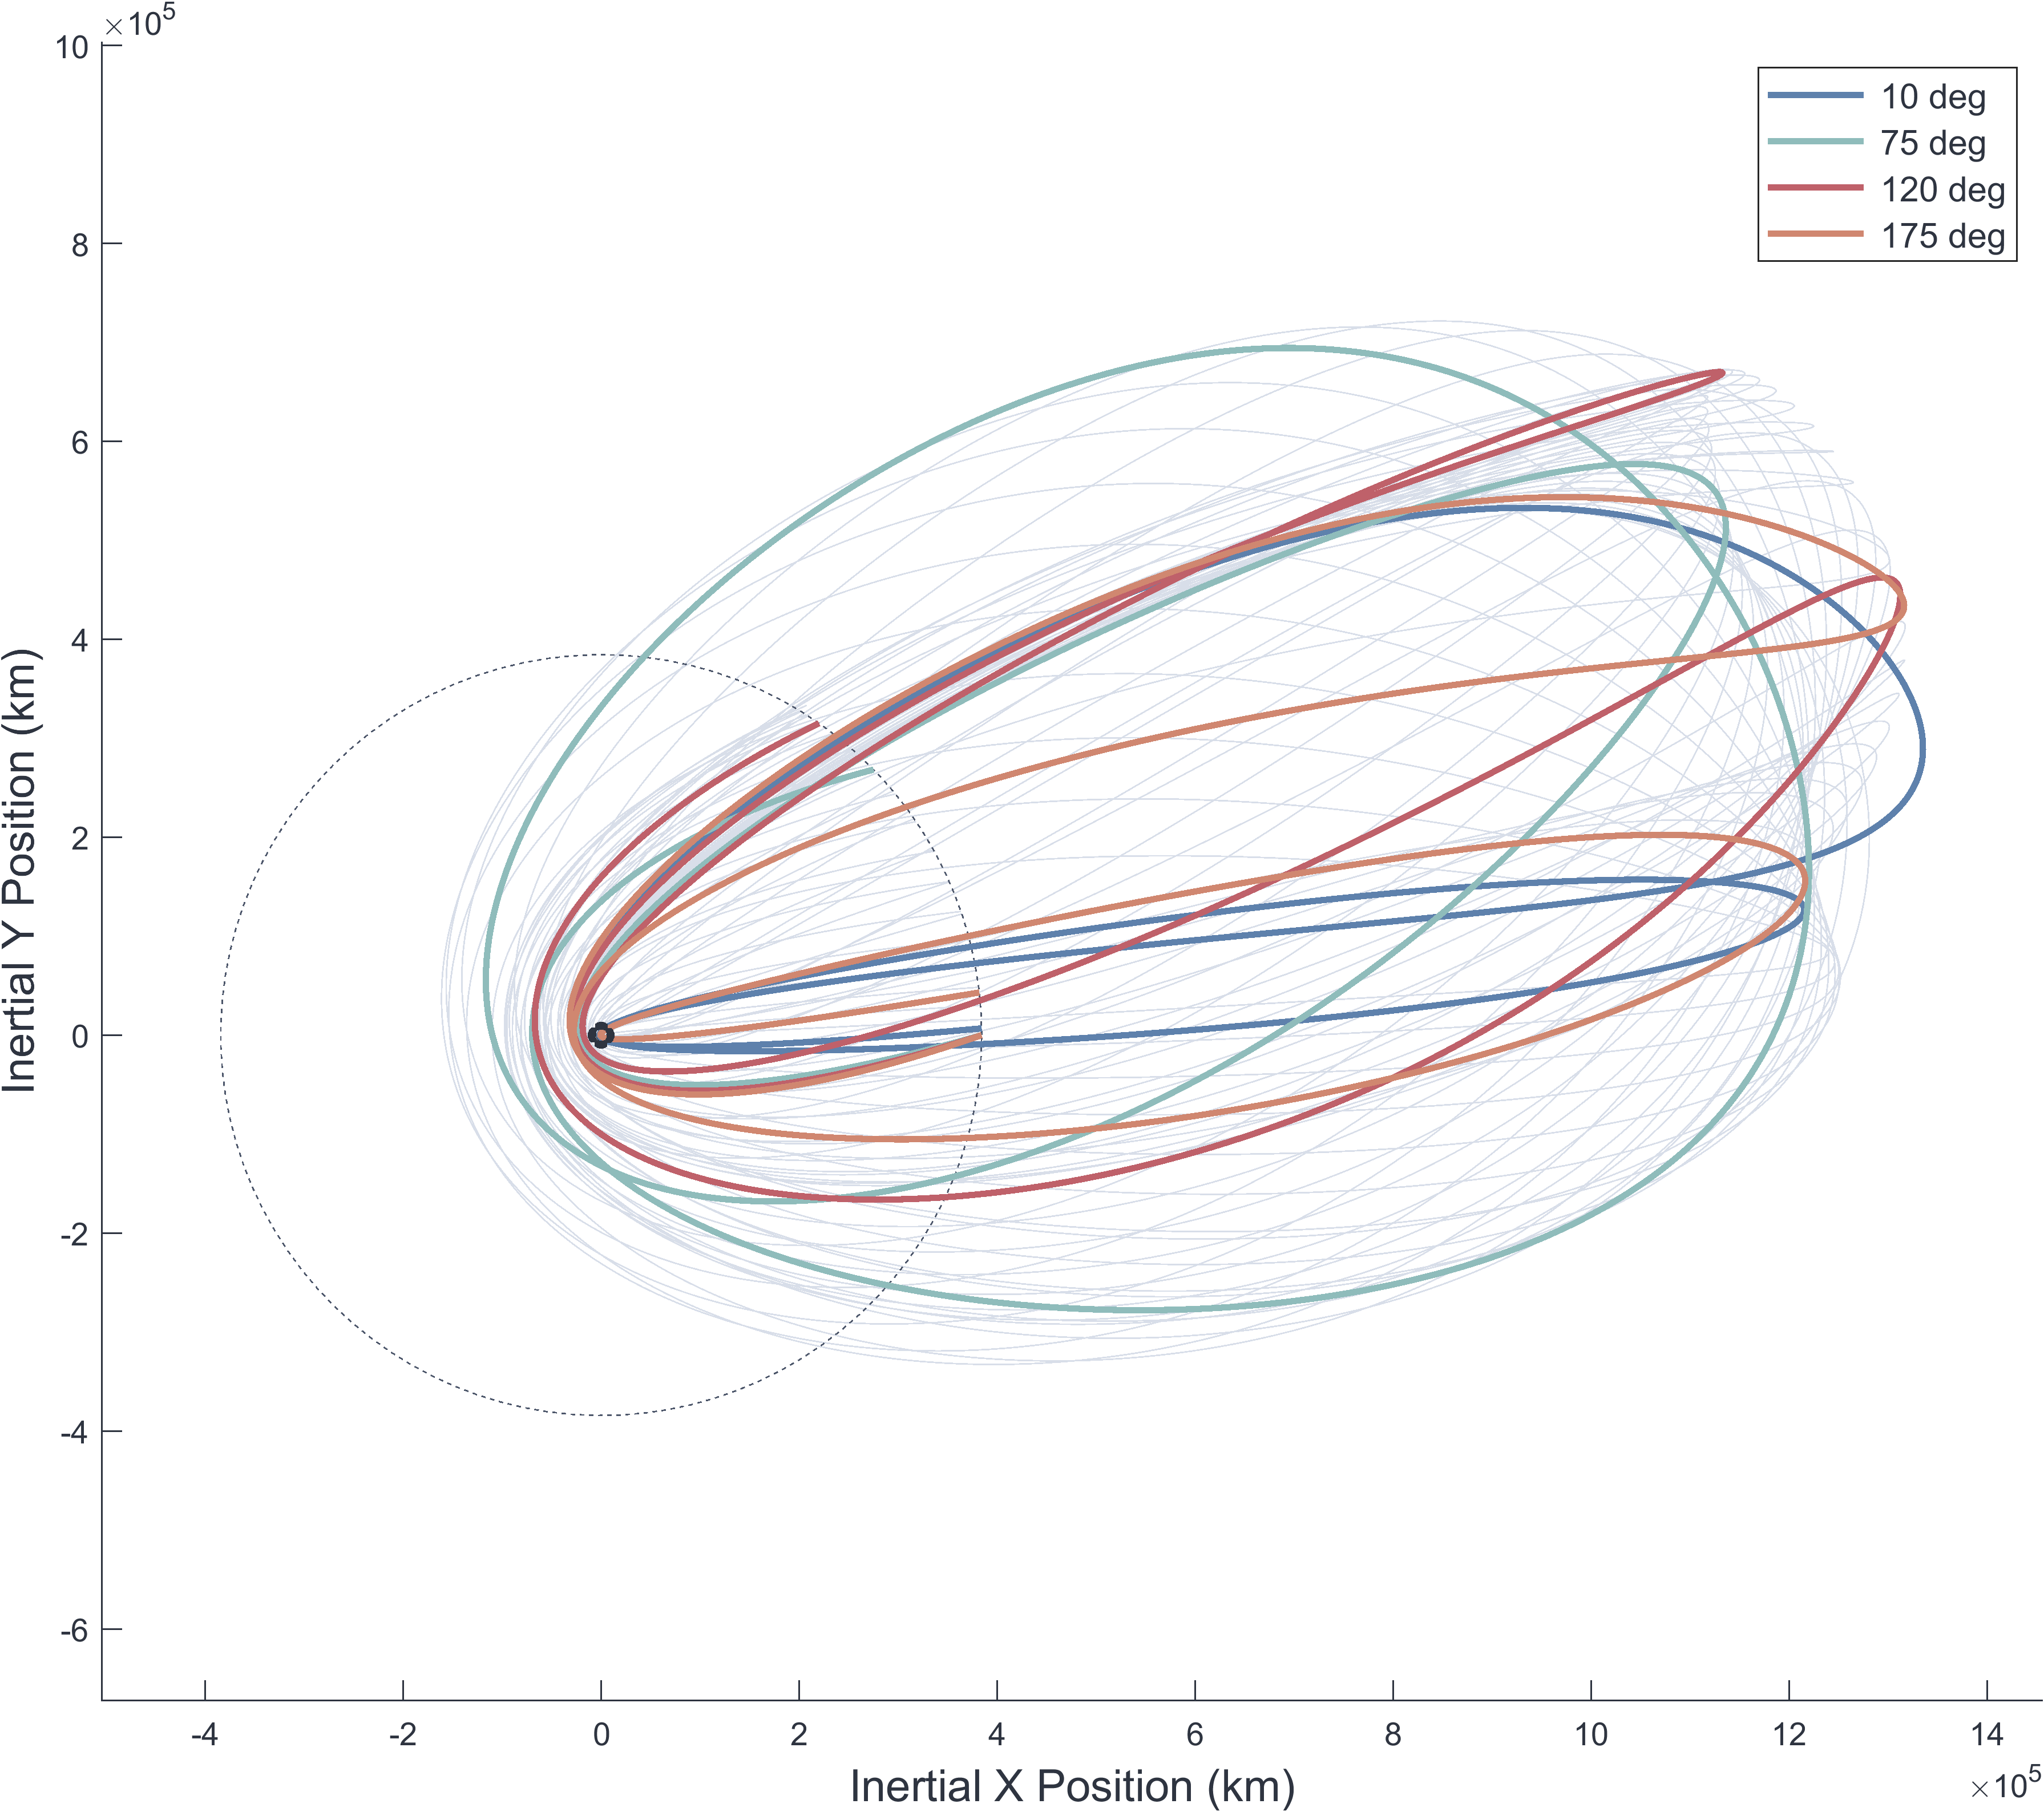
\includegraphics[trim=75 50 0 0, clip, width=2.75in]{./figs/mooni_ThetaPlot_io_famE_vInf1.8.png}
        % \caption{Top 25 results from Europa Clipper dataset, color sorted by sequence}
    \end{subfigure}
    \begin{subfigure}{}
        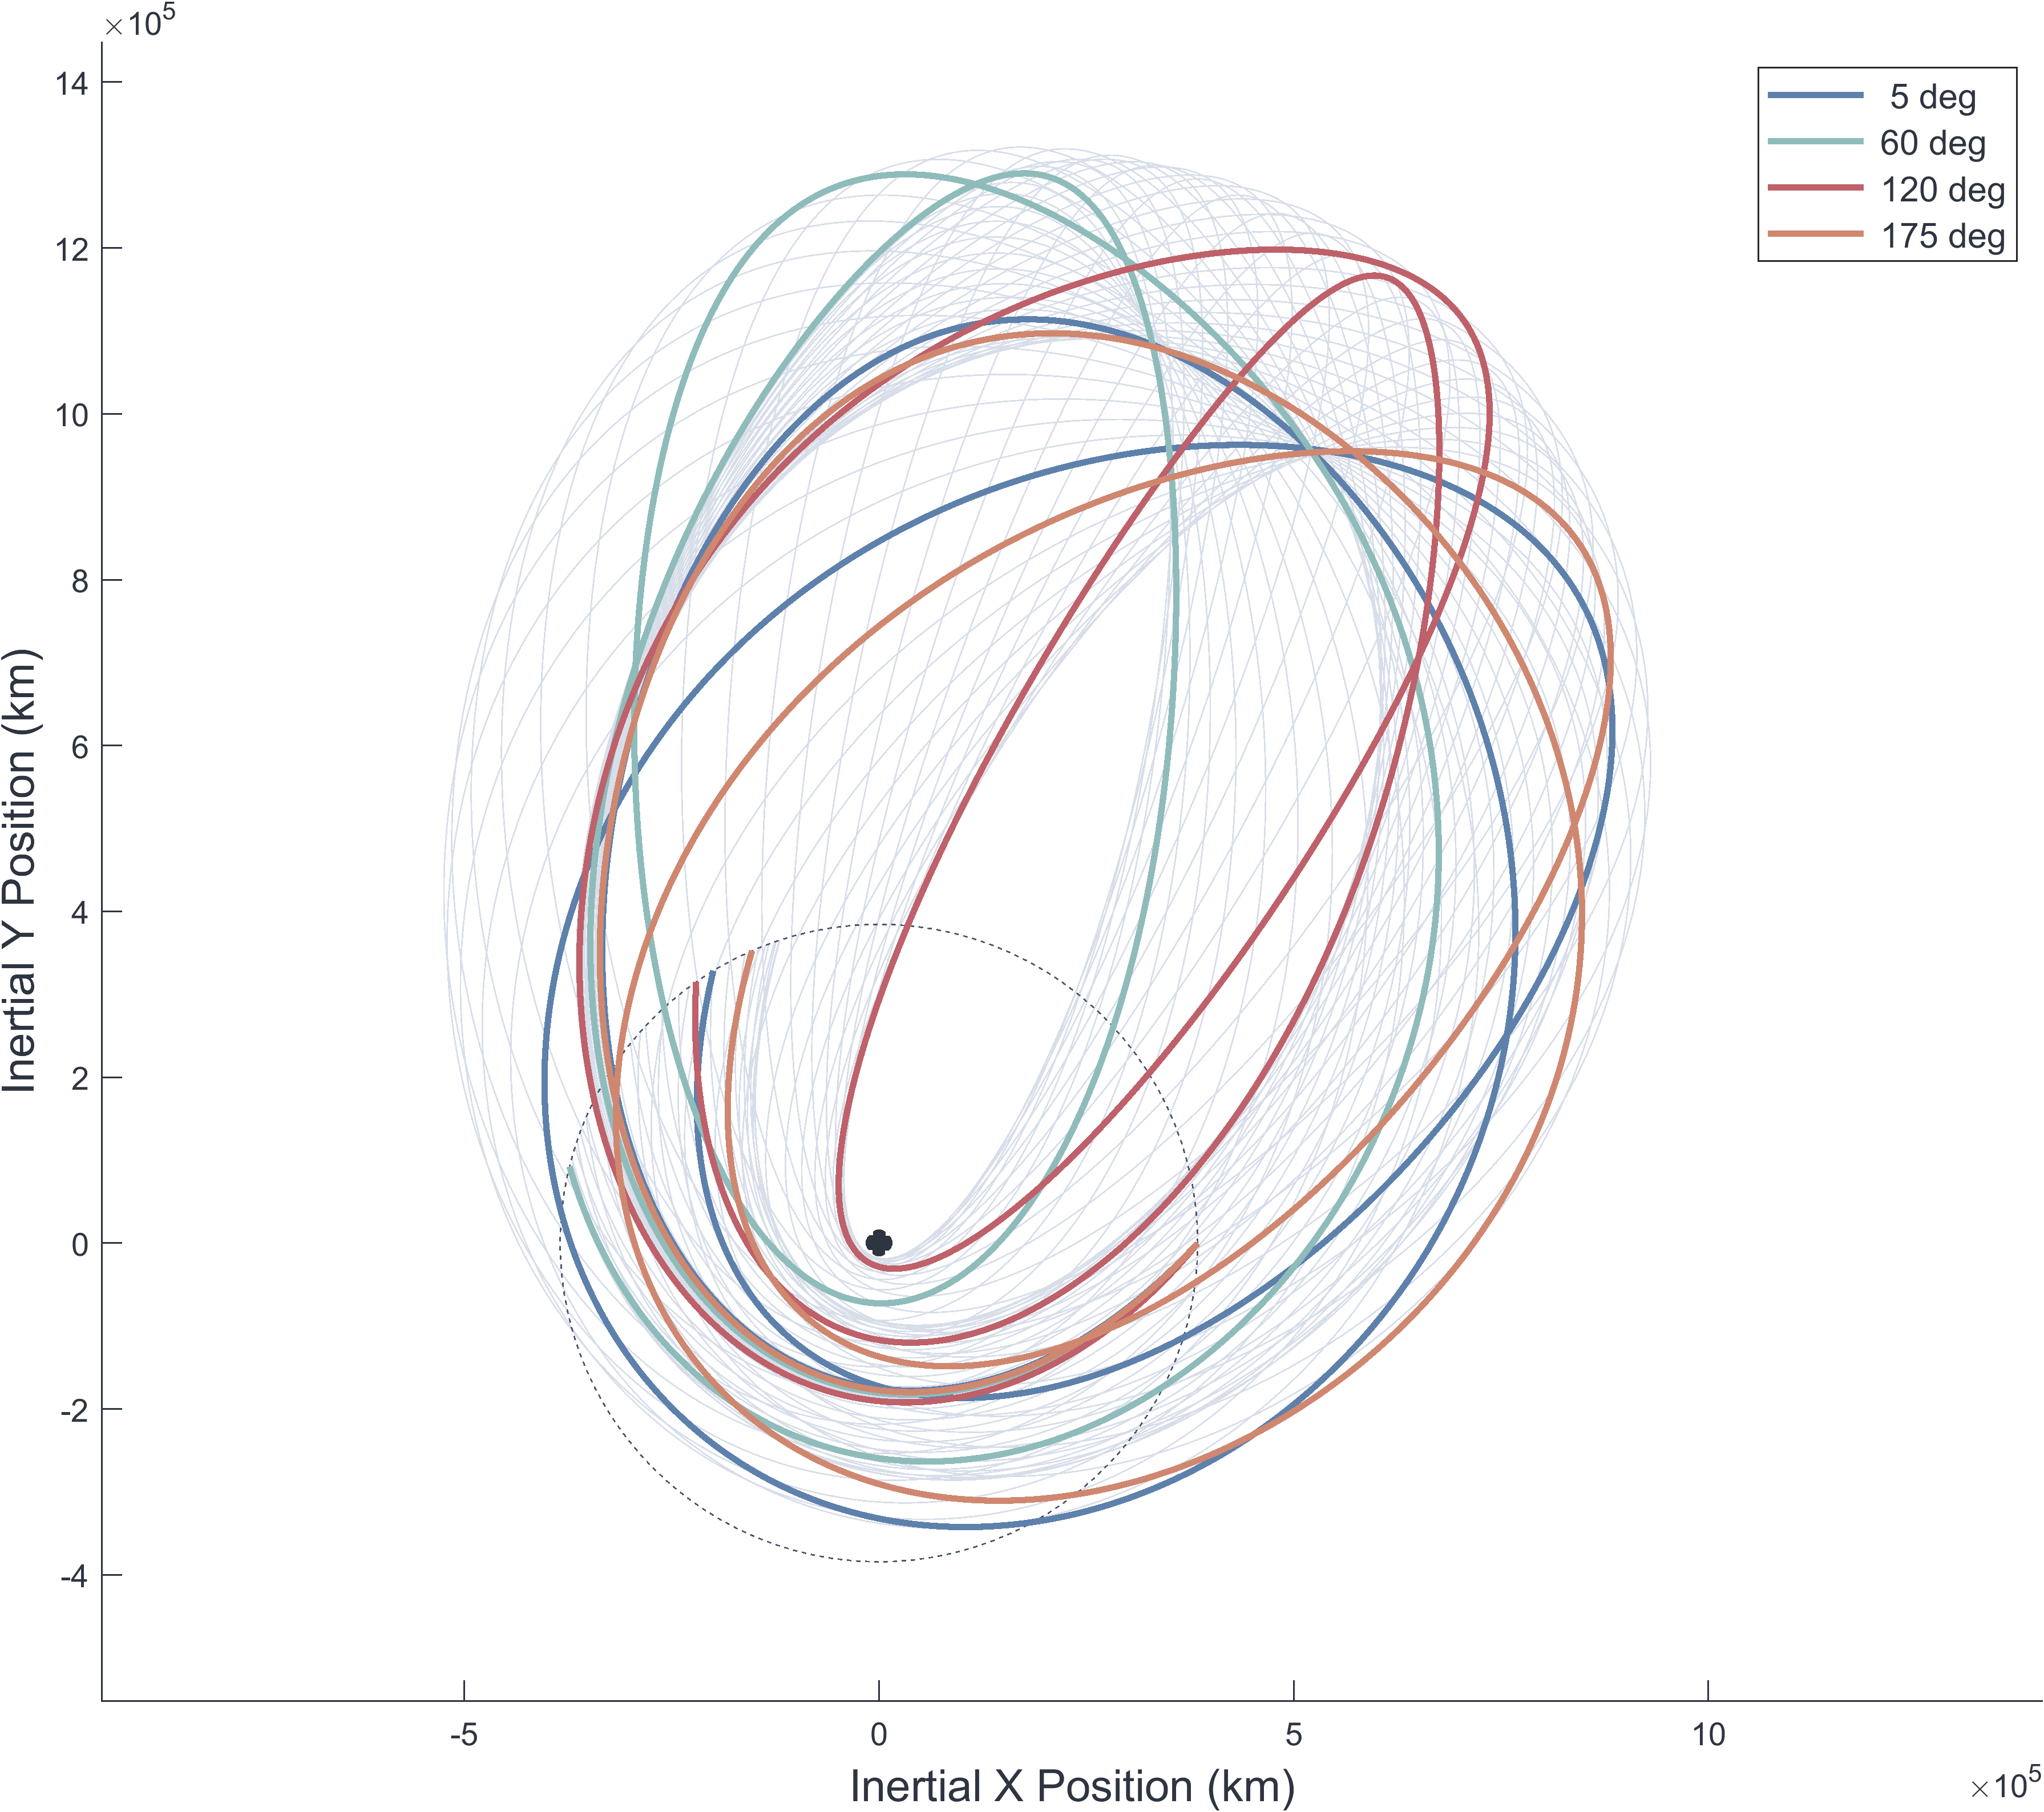
\includegraphics[trim=75 50 0 0, clip, width=2.75in]{./figs/mooni_ThetaPlot_io_famE_vInf2.1.png}
        % \caption{Top 12 results from Galileo dataset, color sorted by sequence}
    \end{subfigure}
    \caption{Progression of Eio family orbits at a v\(_\infty\) of [0.3, 0.6, 0.9, 1.2, 1.8, 2.1] \(^{km}/_s\) as the initial Solar Phase Angles, \(\theta_0\), increases.}
    \label{fig:mooni_thetaPlot_io_E_2.1}
\end{figure}

\clearpage

\subsection*{NEA Scout Trajectory Example}
\pdfbookmark[2]{NEA Scout Trajectory Example}{neascout}

% {\color{cyan} Talk about NEA Scout mission then show trajectory}
As discussed previously, rideshare missions rarely leave the regions where they are initially placed, but with the launch of the Artemis I mission to cislunar space, it will bring along 13 6U cubesats for dispersion. This presents an opportunity for a spacecraft to use Moon-to-Moon transfers to eject itself out of the Earth-Moon system, one such being NEA Scout. This spacecraft is to be used as a testbed for solar sail propulsion and is set to rendezvous with a near-Earth asteroid. 

For an October 2021 launch date, below is one such possible cislunar escape trajectory for the spacecraft. Starting with a Bii, NEA Scout will slowly increase its energy first to a multi-revolution BDii, then to a Dii. From here, the spacecraft would perform on final lunar flyby to put it on a hyperbolic trajectory out of the system into heliocentric space.\footnote{It should be noted all trajectories shown are ballistic and do not utilize the solar sail in any way.} Patching together cislunar trajectories is accomplished through two-body patch conics approximations using hyperbolic trajectories around the Moon. As the \textbf{v}\(_\infty\) is known at each end of the trajectory, all values necessary to calculate the validity of such a lunar flyby are easily accessible. Firstly, the magnitudes of the \textbf{v}\(_\infty\) in and out of the lunar encountered are compared and made sure to be within bounds of one another. If so, the \textbf{v}\(_\infty\)'s are then used to make a feasibility check on the hyperbolic orbit's bend angle, and avoid any surface impacts. 

\begin{figure}[h]
    \centering
    \begin{subfigure}
        \centering
        % \vspace{0.5in}
        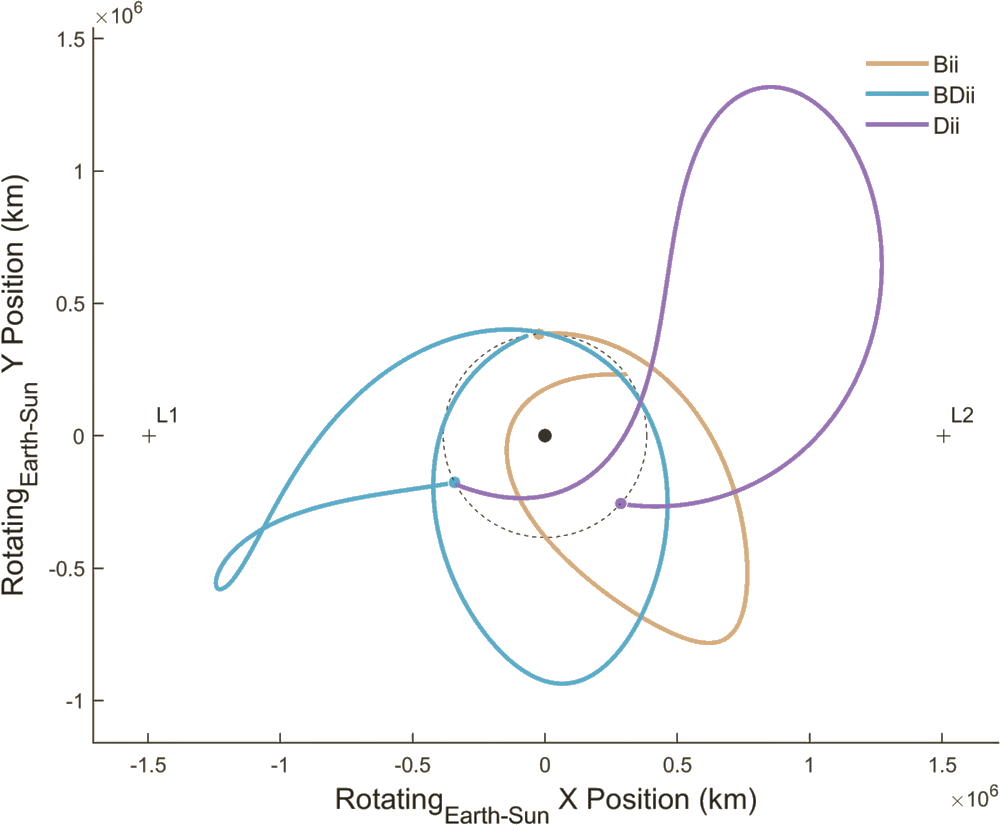
\includegraphics[width=3in]{./etc/figure13-2.png}
    \end{subfigure}
    \begin{subfigure}
        \centering
        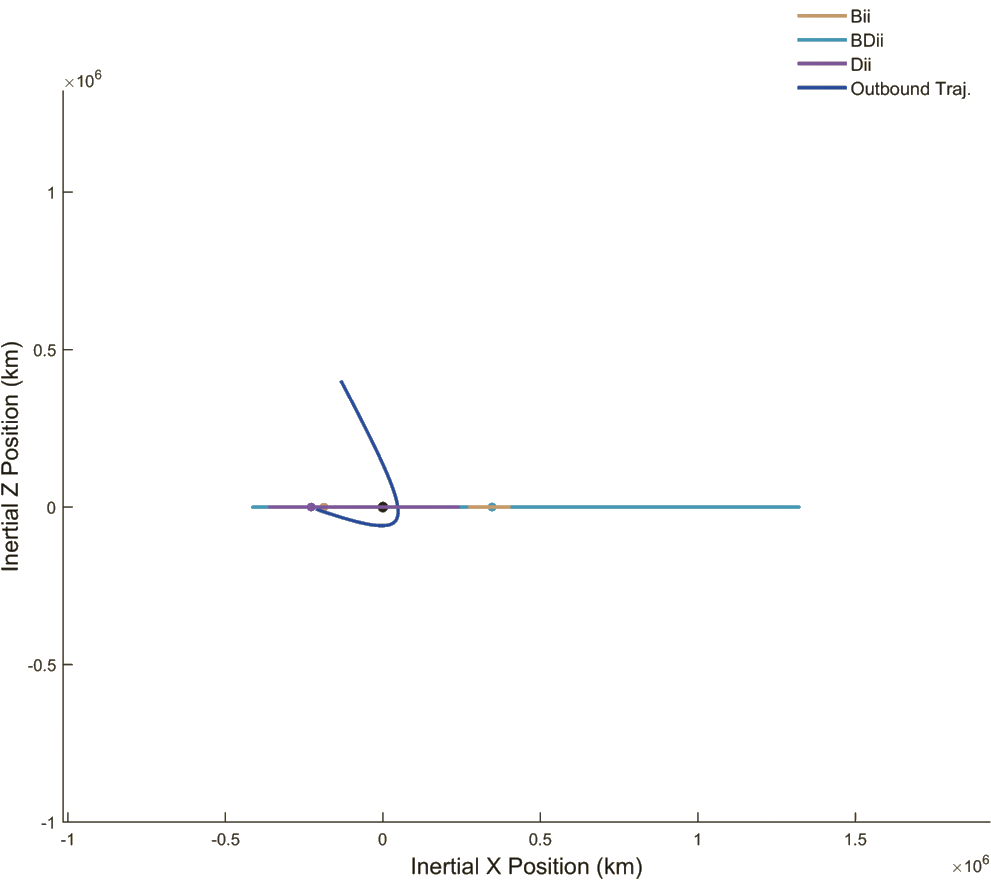
\includegraphics[width=2.7in]{./etc/figure9-2.png}
    \end{subfigure}
    \caption{(Left) One possible NEA Scout Trajectory in the Sun-Earth Rotating Frame. (Right) Outbound leg of trajectory in Earth-Centered Inertial Frame.}
    \label{fig:neascout}
\end{figure}

\section*{Conclusions}
\pdfbookmark[1]{Conclusions}{conc}
Multi-revolution Moon-to-Moon trajectories provide a new avenue of opportunities for mission designers already operating within cislunar space. In this paper, we defined a method for calculating and building zero and multi-revolution trajectory families. The inclusion of multi-revolution trajectories proved to increase the number of possible transfers for a given initial trajectory state. This added flexibility gives more latitude to mission designers to meet their mission criteria. Such cislunar trajectories are especially valuable to rideshare mission types as the launch date is predetermined. These benefits can be applied to any future rideshare missions that need to escape from cislunar to heliocentric space. In particular, the NEA Scout mission is exploiting these trajectories to escape the Earth-Moon system and rendezvous with a Near-Earth asteroid.

\section*{Acknowledgements}
This research was carried out at the Jet Propulsion Laboratory, California Institute of Technology, and is made available for information purposes only. Reference to any specific commercial
product, process, or service by trade name, trademark, manufacturer or otherwise, does not constitute or imply its endorsement by the United States Government or the Jet Propulsion Laboratory,
California Institute of Technology. Copyright 2021 California Institute of Technology. Government sponsorship acknowledged.

\appendix
\clearpage
\section*{Appendix A: Family Plots in the Sun-Earth Rotating Frame}
\label{section:appA}
\pdfbookmark[1]{Appendix A: Family Plots in the Sun-Earth Rotating Frame}{appendixA}
% ROTATING PLOTS


\begin{figure}[h!]
    \begin{subfigure}{}
        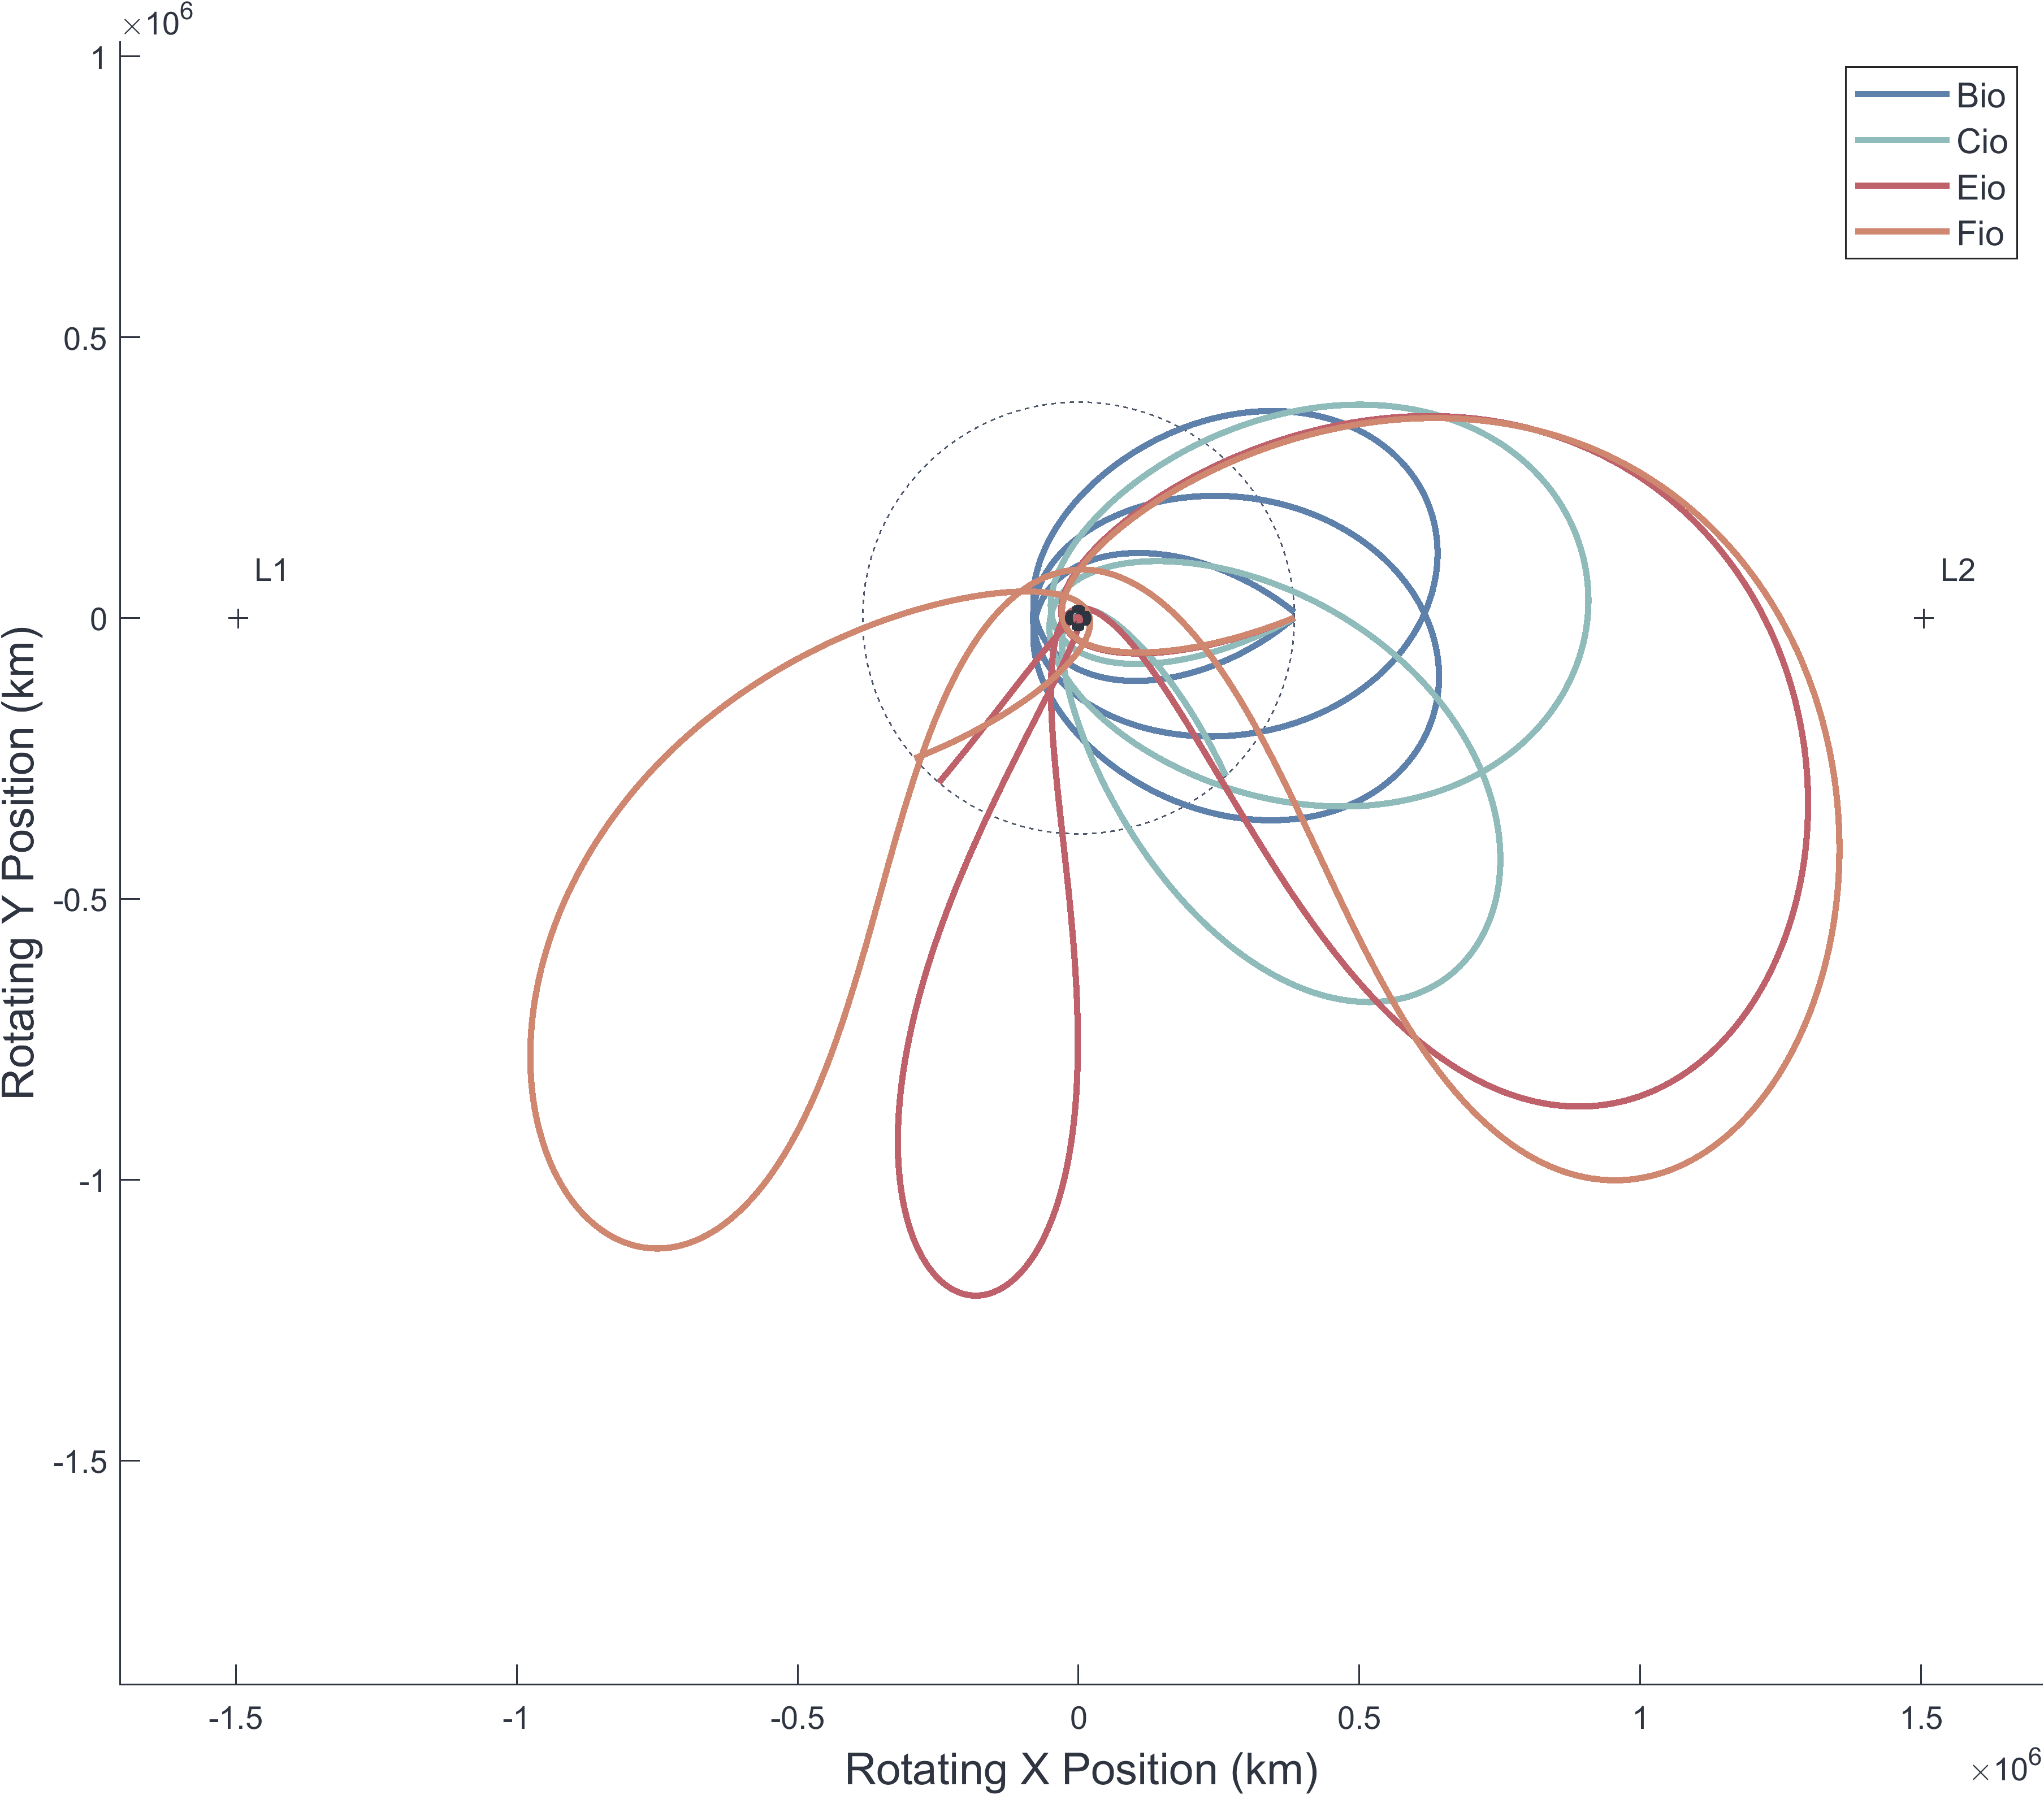
\includegraphics[trim=75 50 0 0, clip, width=3in]{./figs/sunrot_FamilyPlot_io_vInf1.8_theta0.png}
        % \caption{Top 25 results from Europa Clipper dataset, color sorted by sequence}
    \end{subfigure}
    \begin{subfigure}{}
        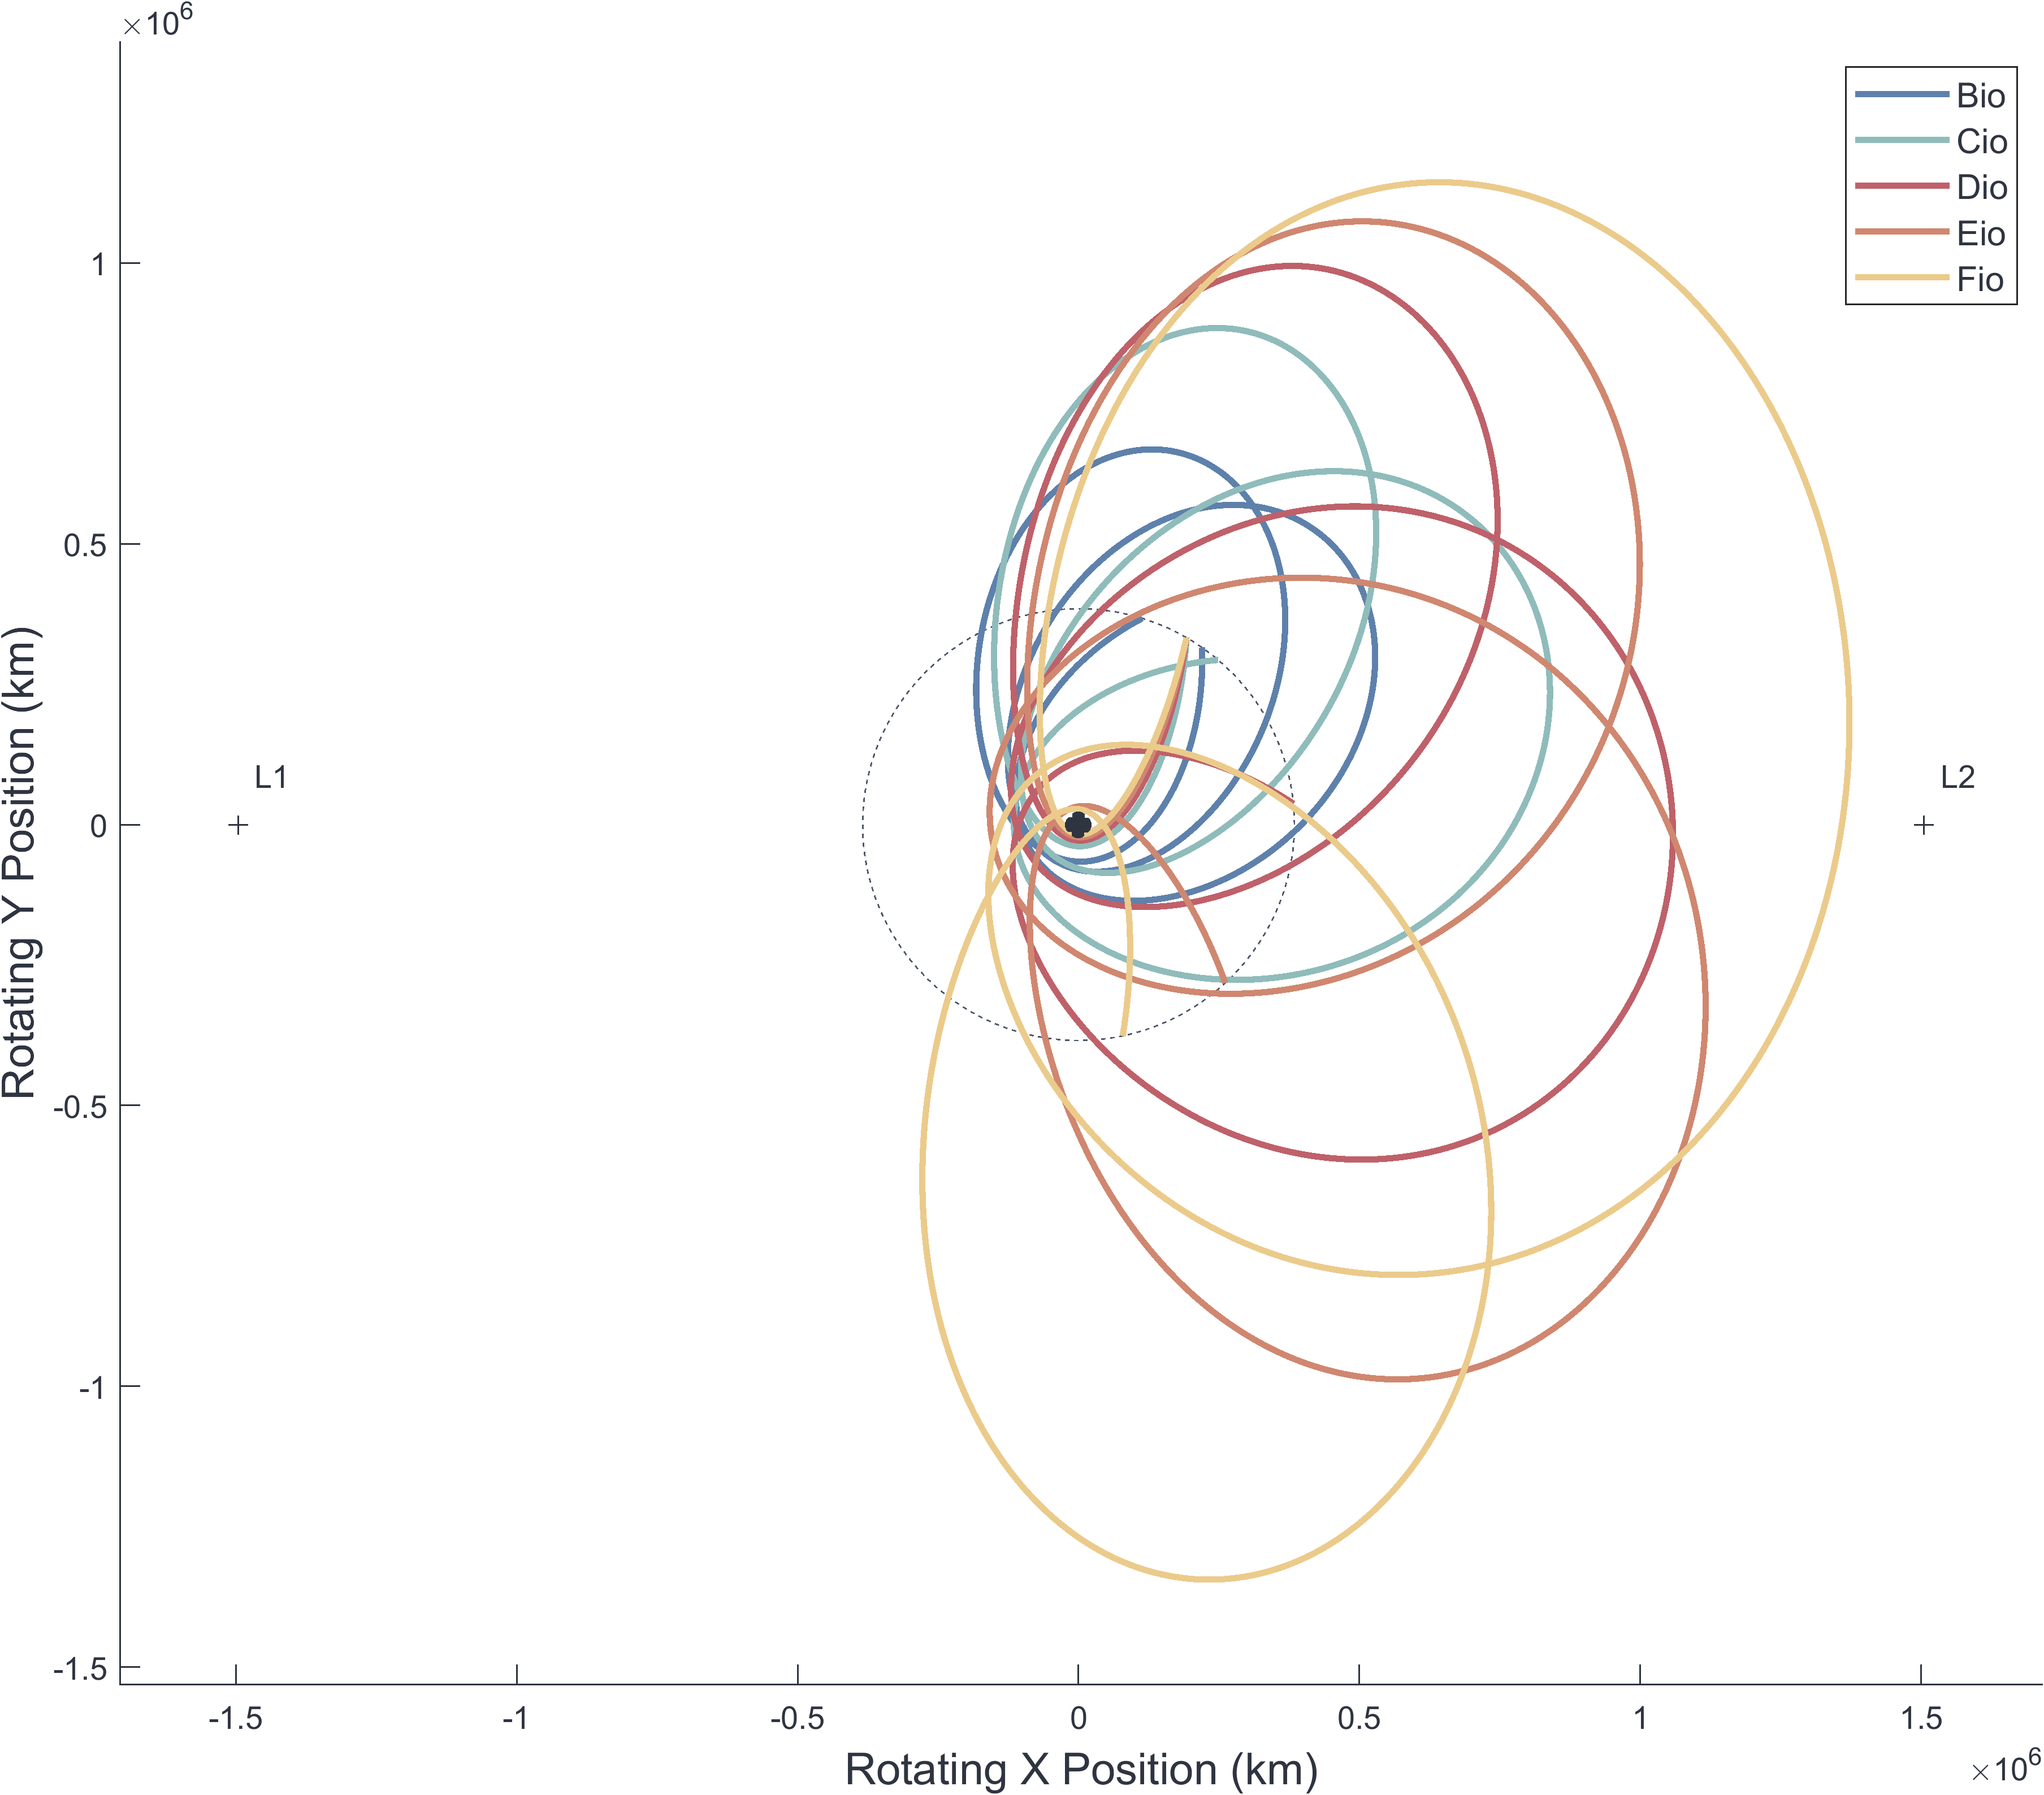
\includegraphics[trim=75 50 0 0, clip, width=3in]{./figs/sunrot_FamilyPlot_io_vInf1.8_theta60.png}
        % \caption{Top 12 results from Galileo dataset, color sorted by sequence}
    \end{subfigure}
\end{figure}
\begin{figure}[h]
    \centering
    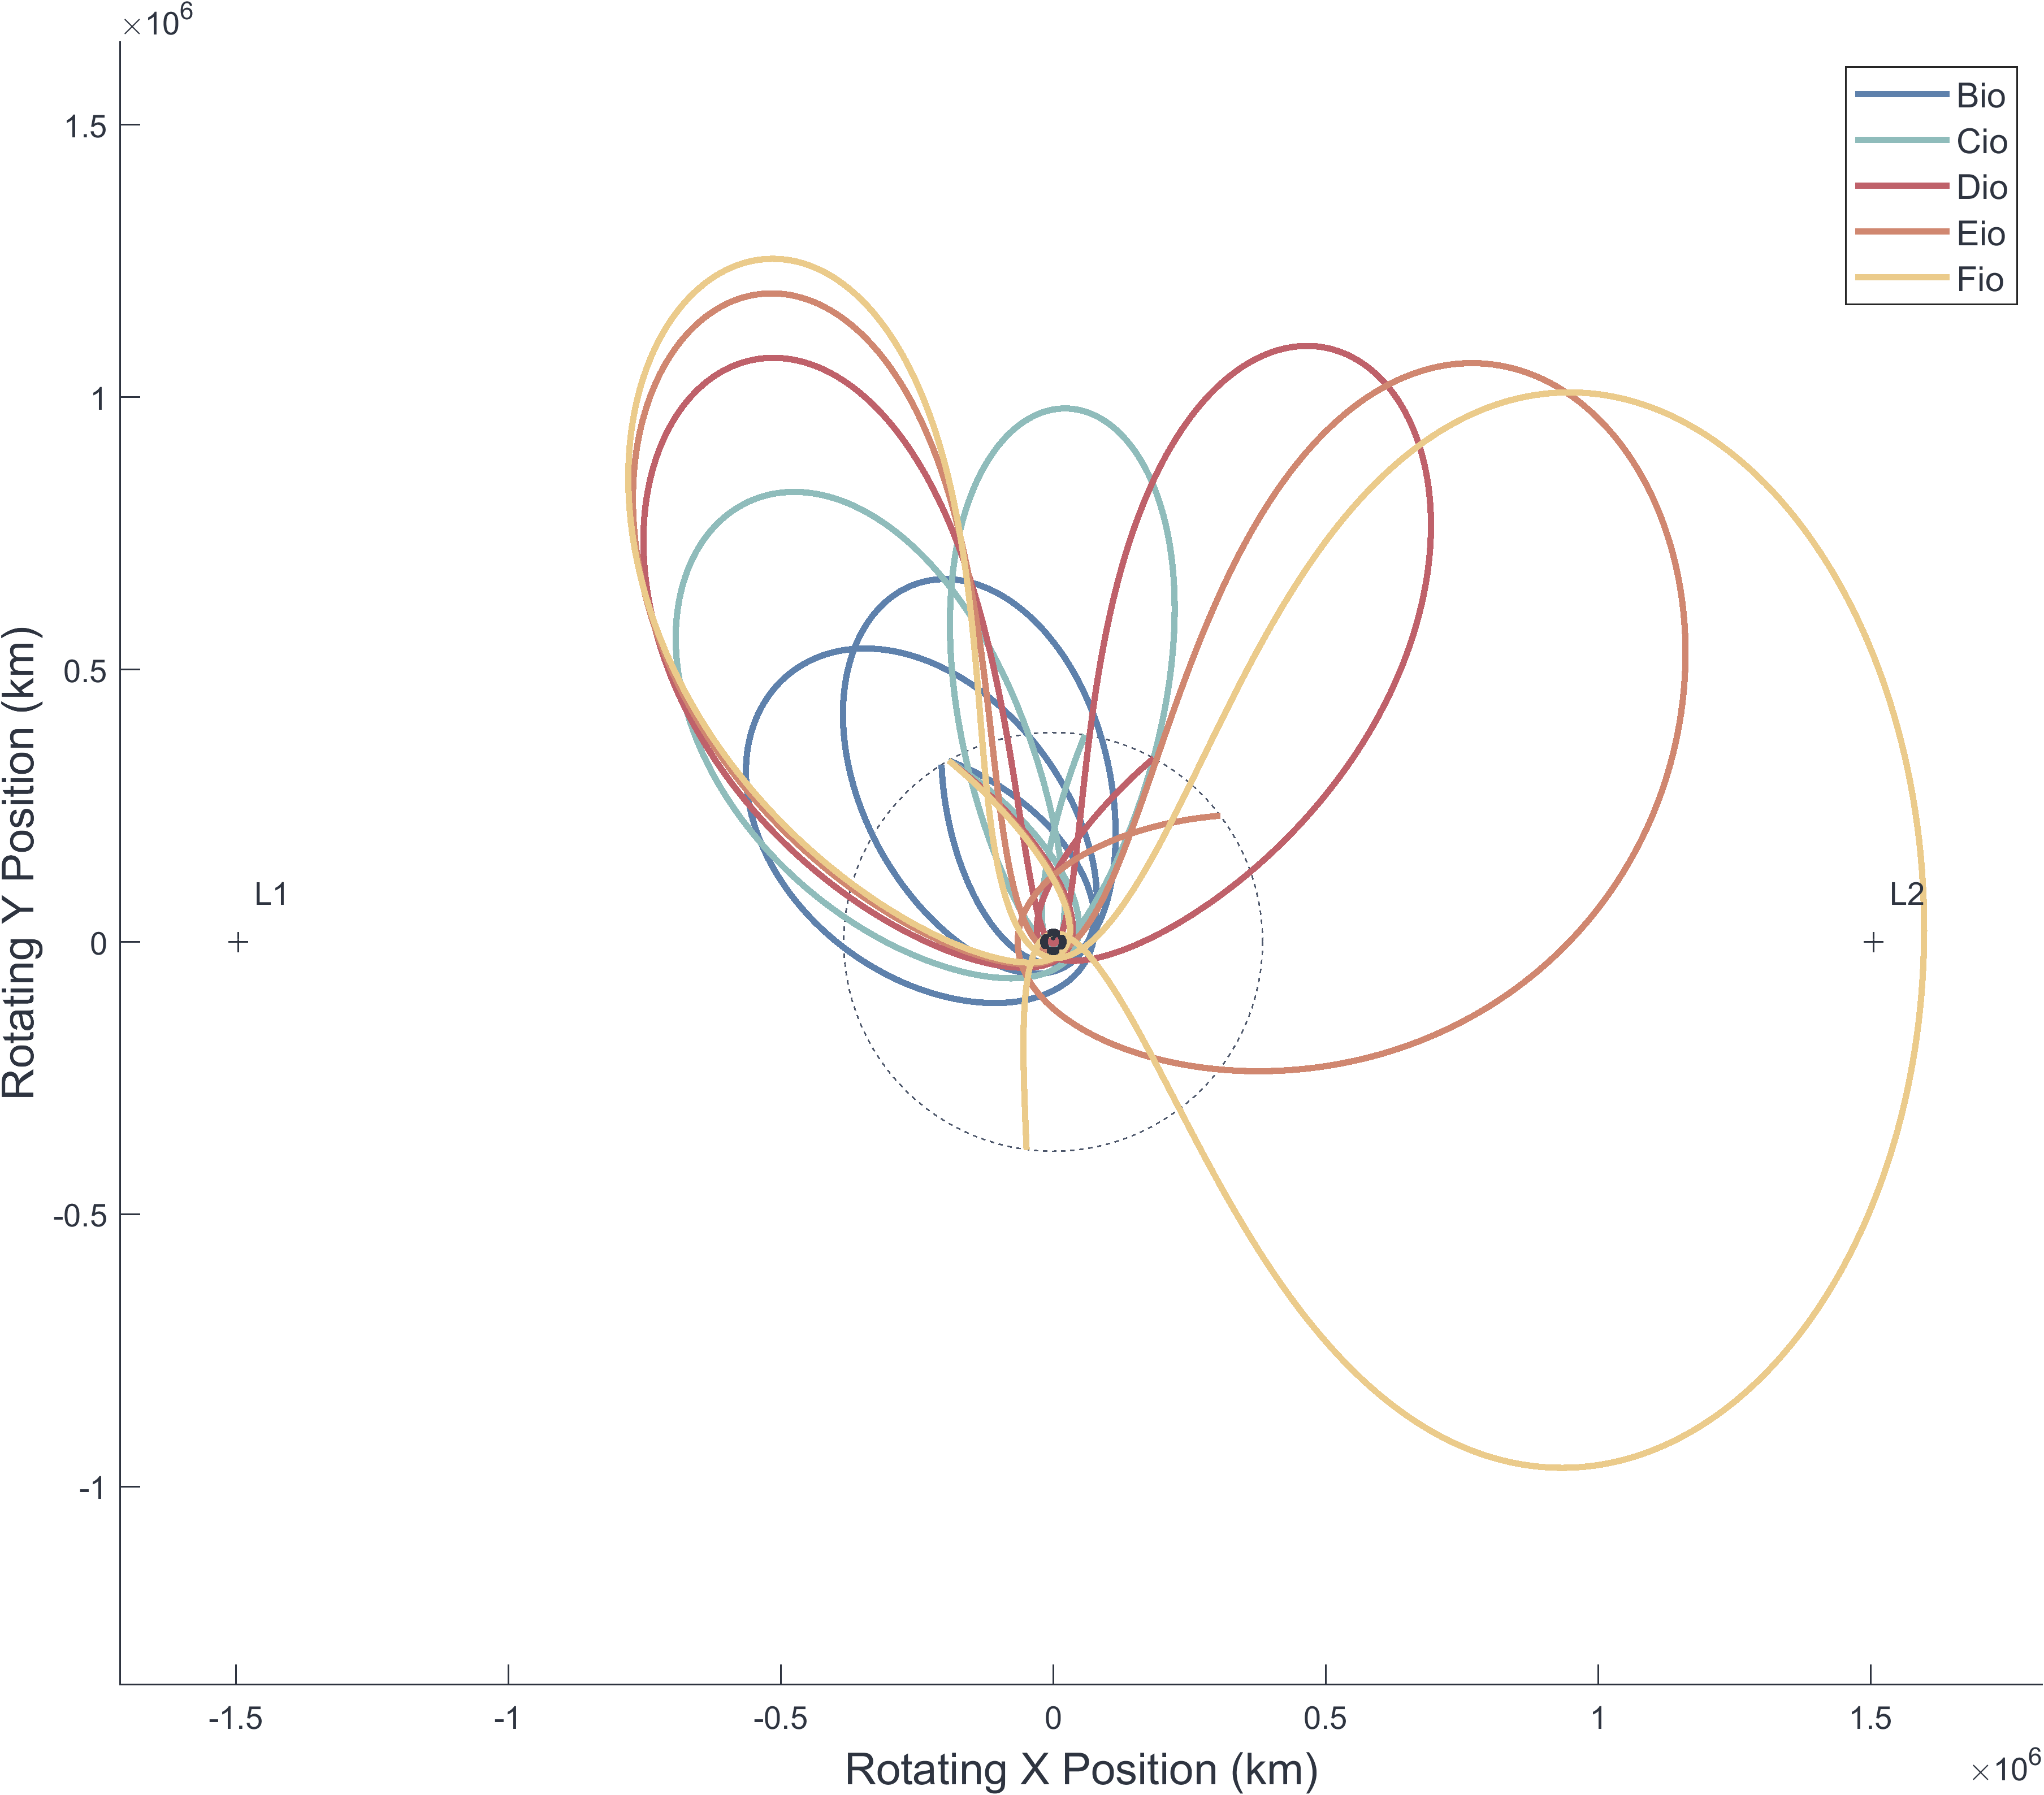
\includegraphics[trim=75 50 0 0, clip, width=3in]{./figs/sunrot_FamilyPlot_io_vInf1.8_theta120.png}
    \caption{Progression of io family orbits at a v\(_\infty\) of 1.8 \(^{km}/_s\) as time of flight is increased across initial Solar Phase Angles, \(\theta_0\), of 0°, 60°, and 120°. It can be more clearly seen, compared to inertial orbits, that the structure between each time of flight progression modifies the structures in each revolutions loop slightly. }
    \label{fig:sunrot_famPlot_io_1.8}
\end{figure}


\begin{figure}[h!]
    \begin{subfigure}{}
        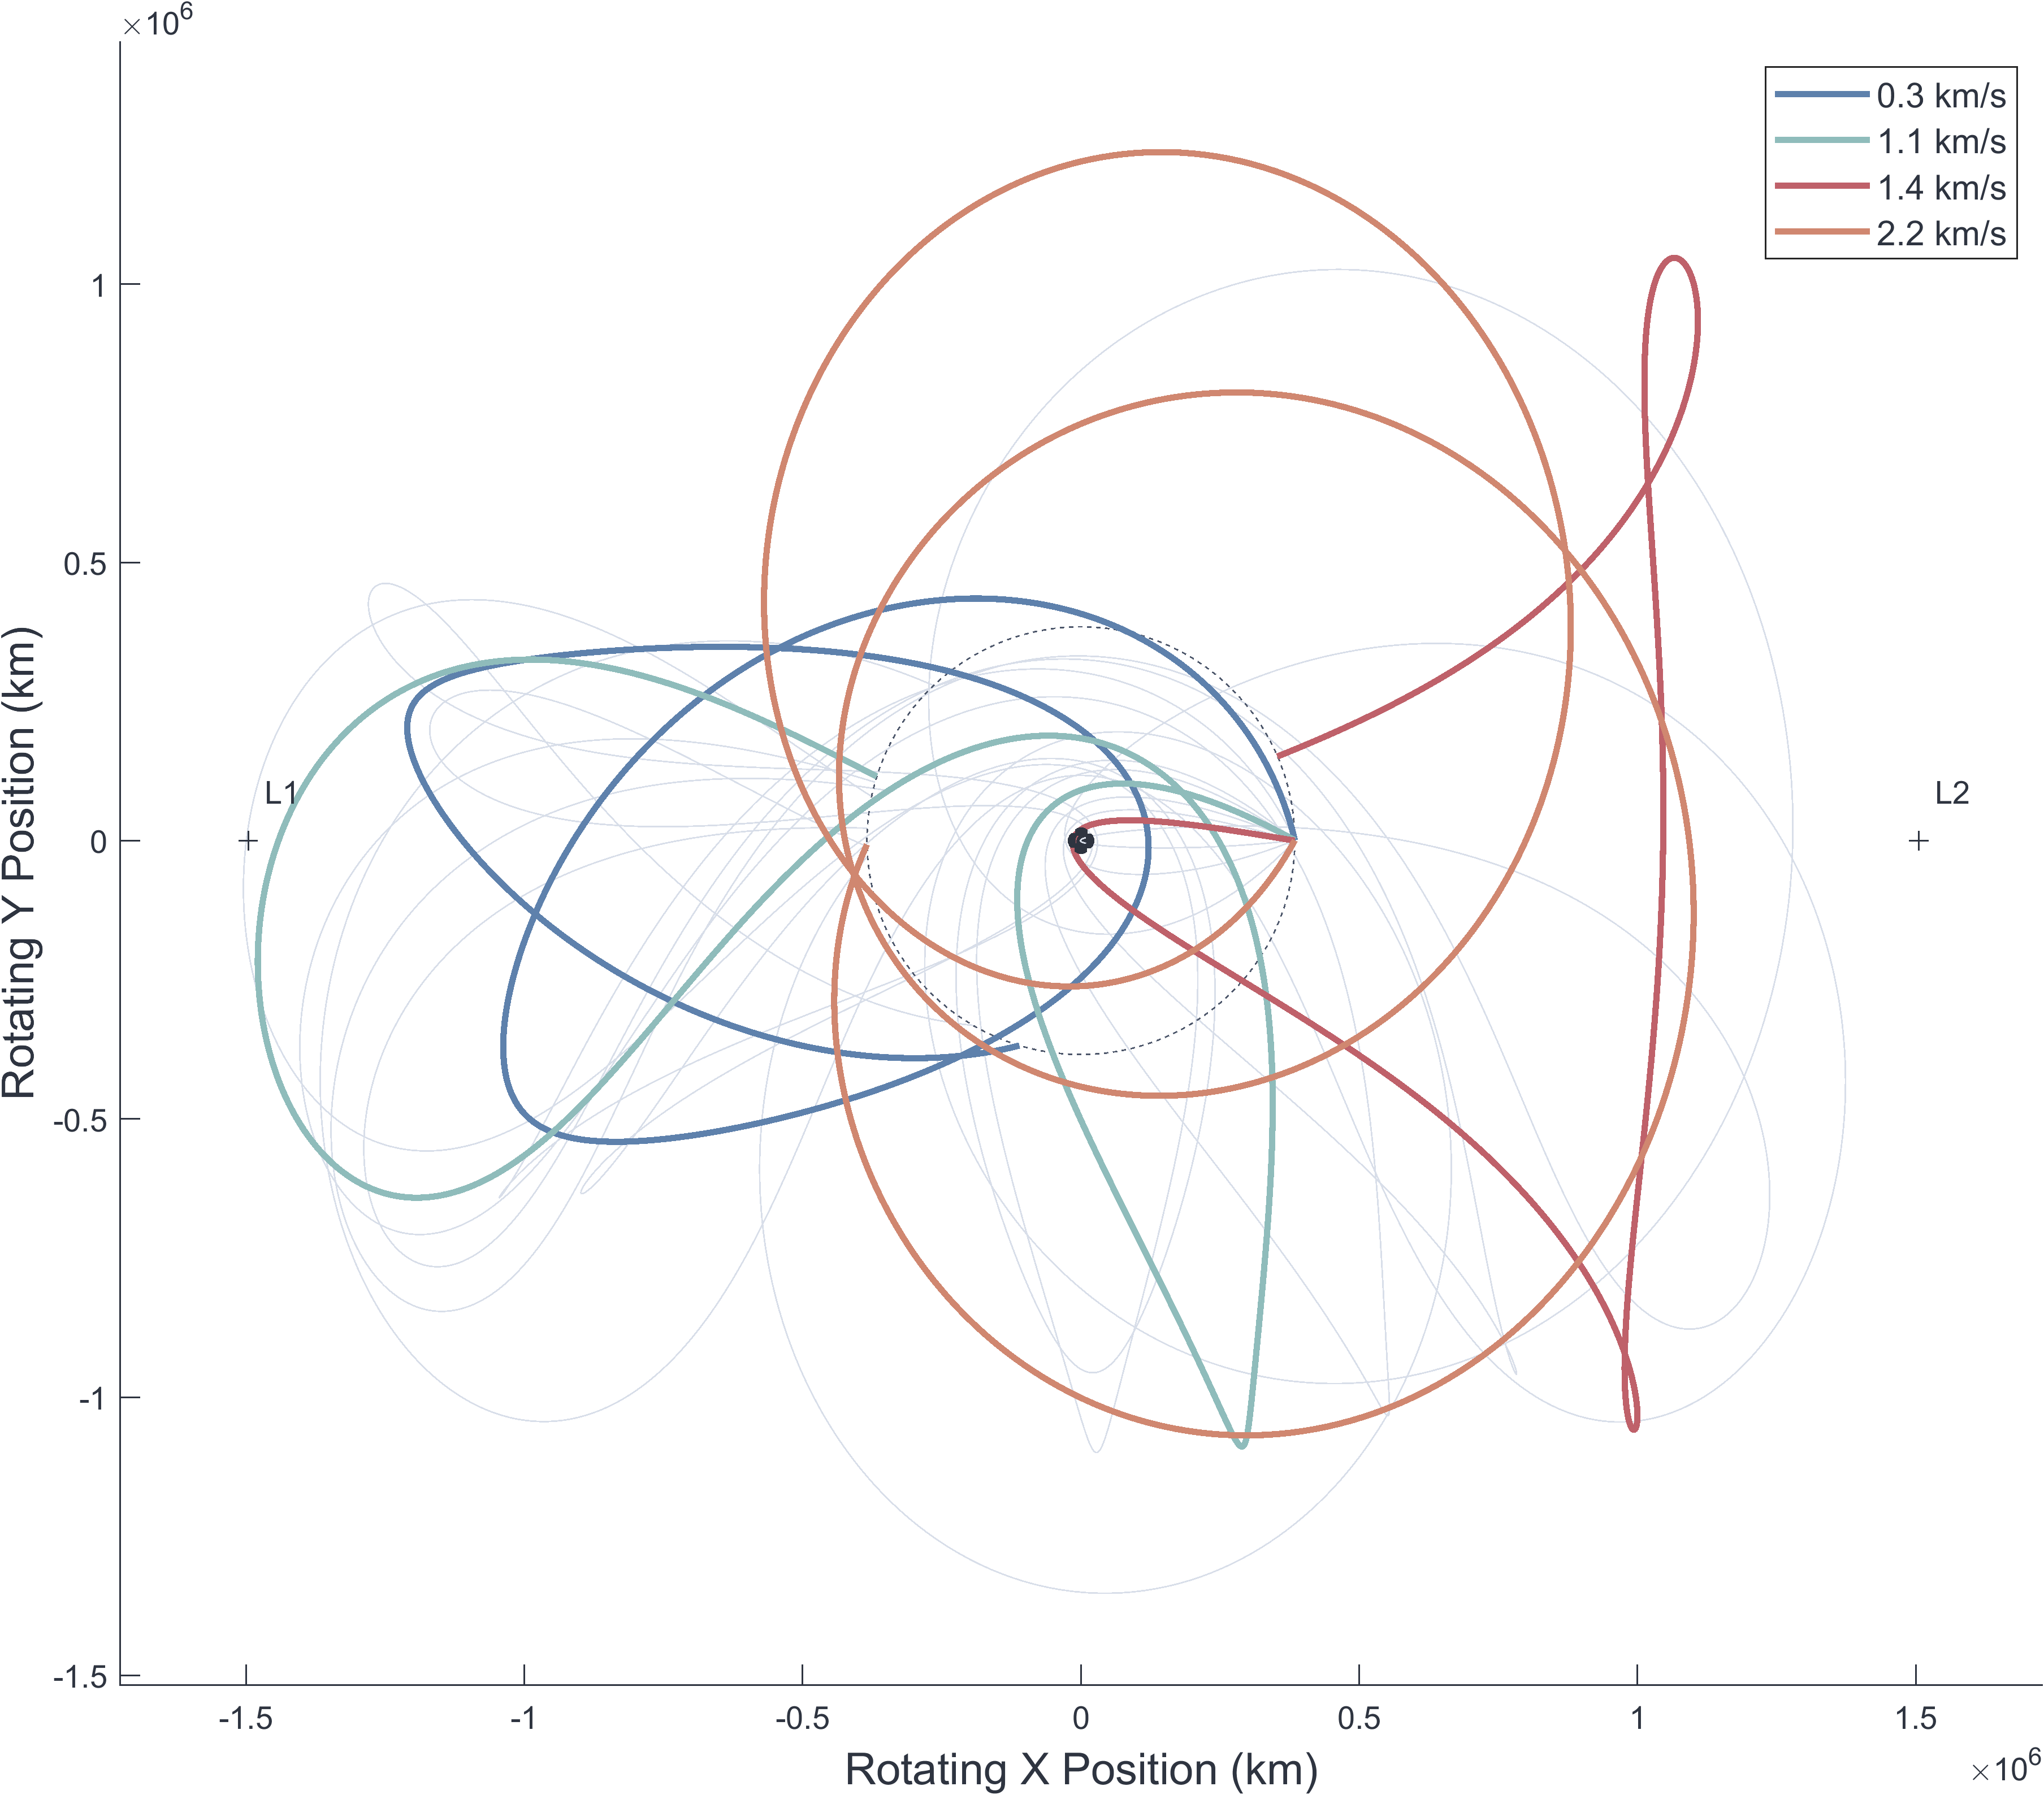
\includegraphics[trim=75 50 0 0, clip, width=3in]{./figs/sunrot_vInfPlot_ii_famF_theta0.png}
        % \caption{Top 25 results from Europa Clipper dataset, color sorted by sequence}
    \end{subfigure}
    \begin{subfigure}{}
        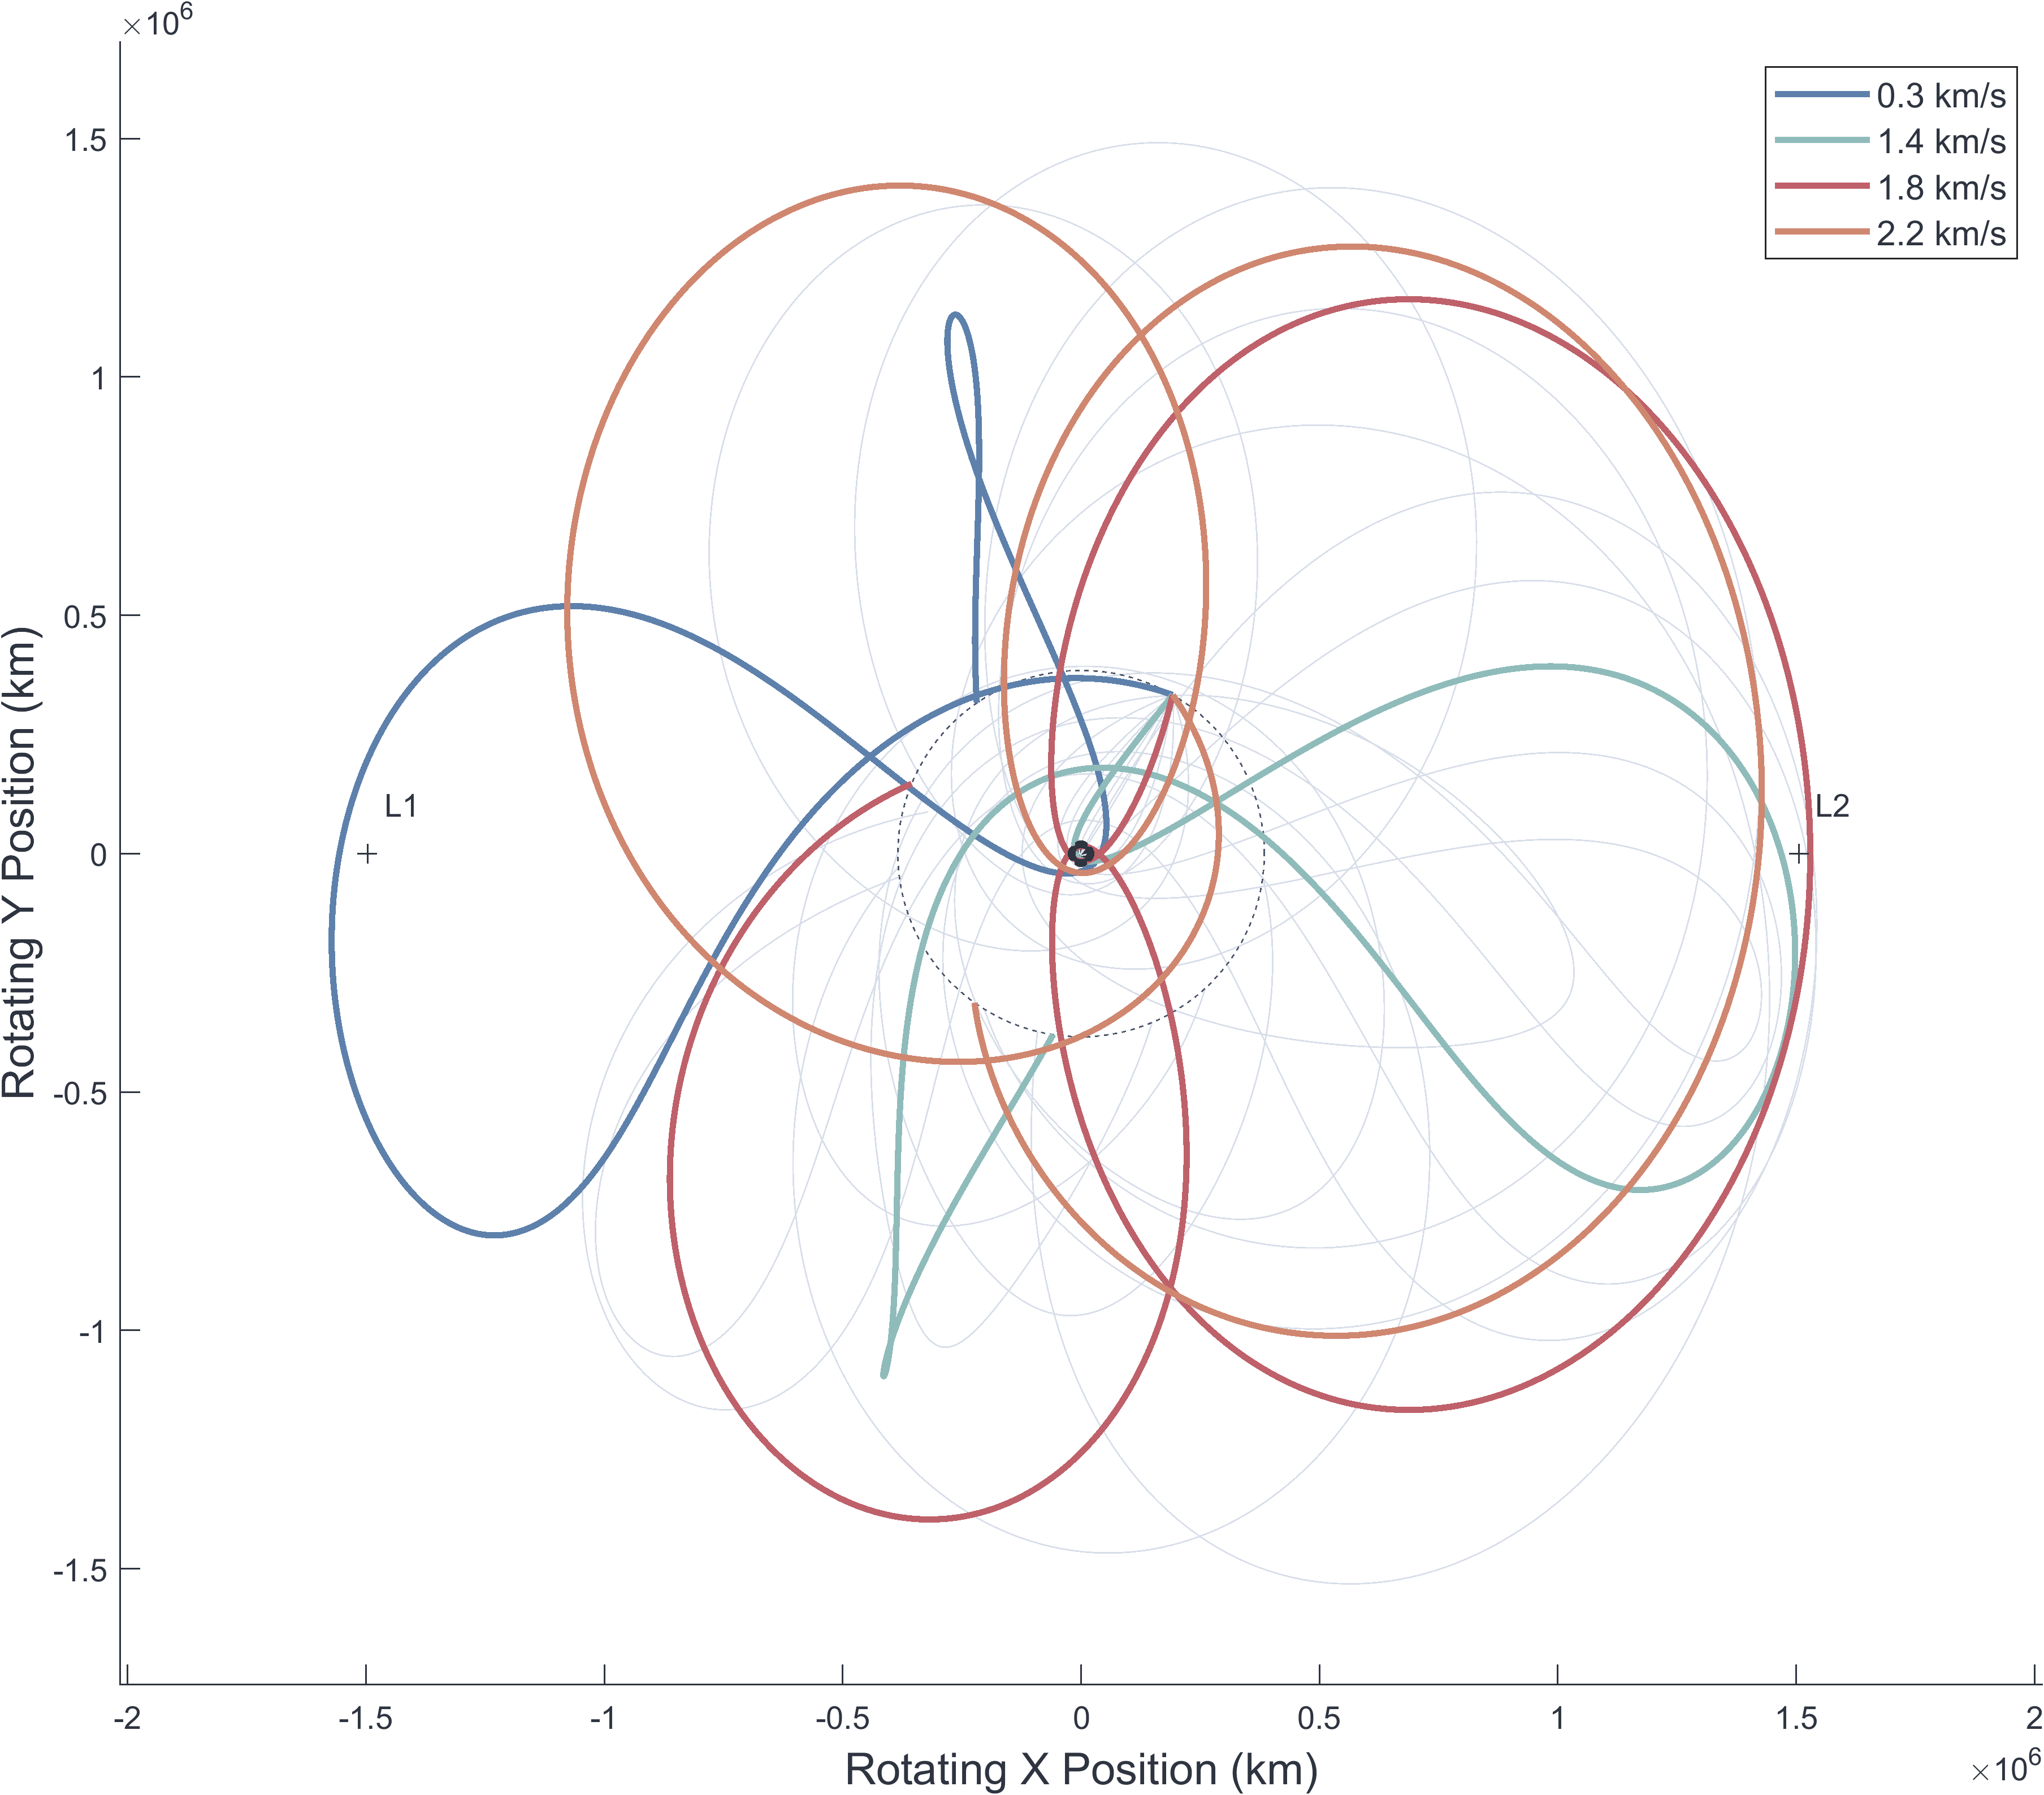
\includegraphics[trim=75 50 0 0, clip, width=3in]{./figs/sunrot_vInfPlot_ii_famF_theta60.png}
        % \caption{Top 12 results from Galileo dataset, color sorted by sequence}
    \end{subfigure}
\end{figure}
\begin{figure}[h]
    \centering
    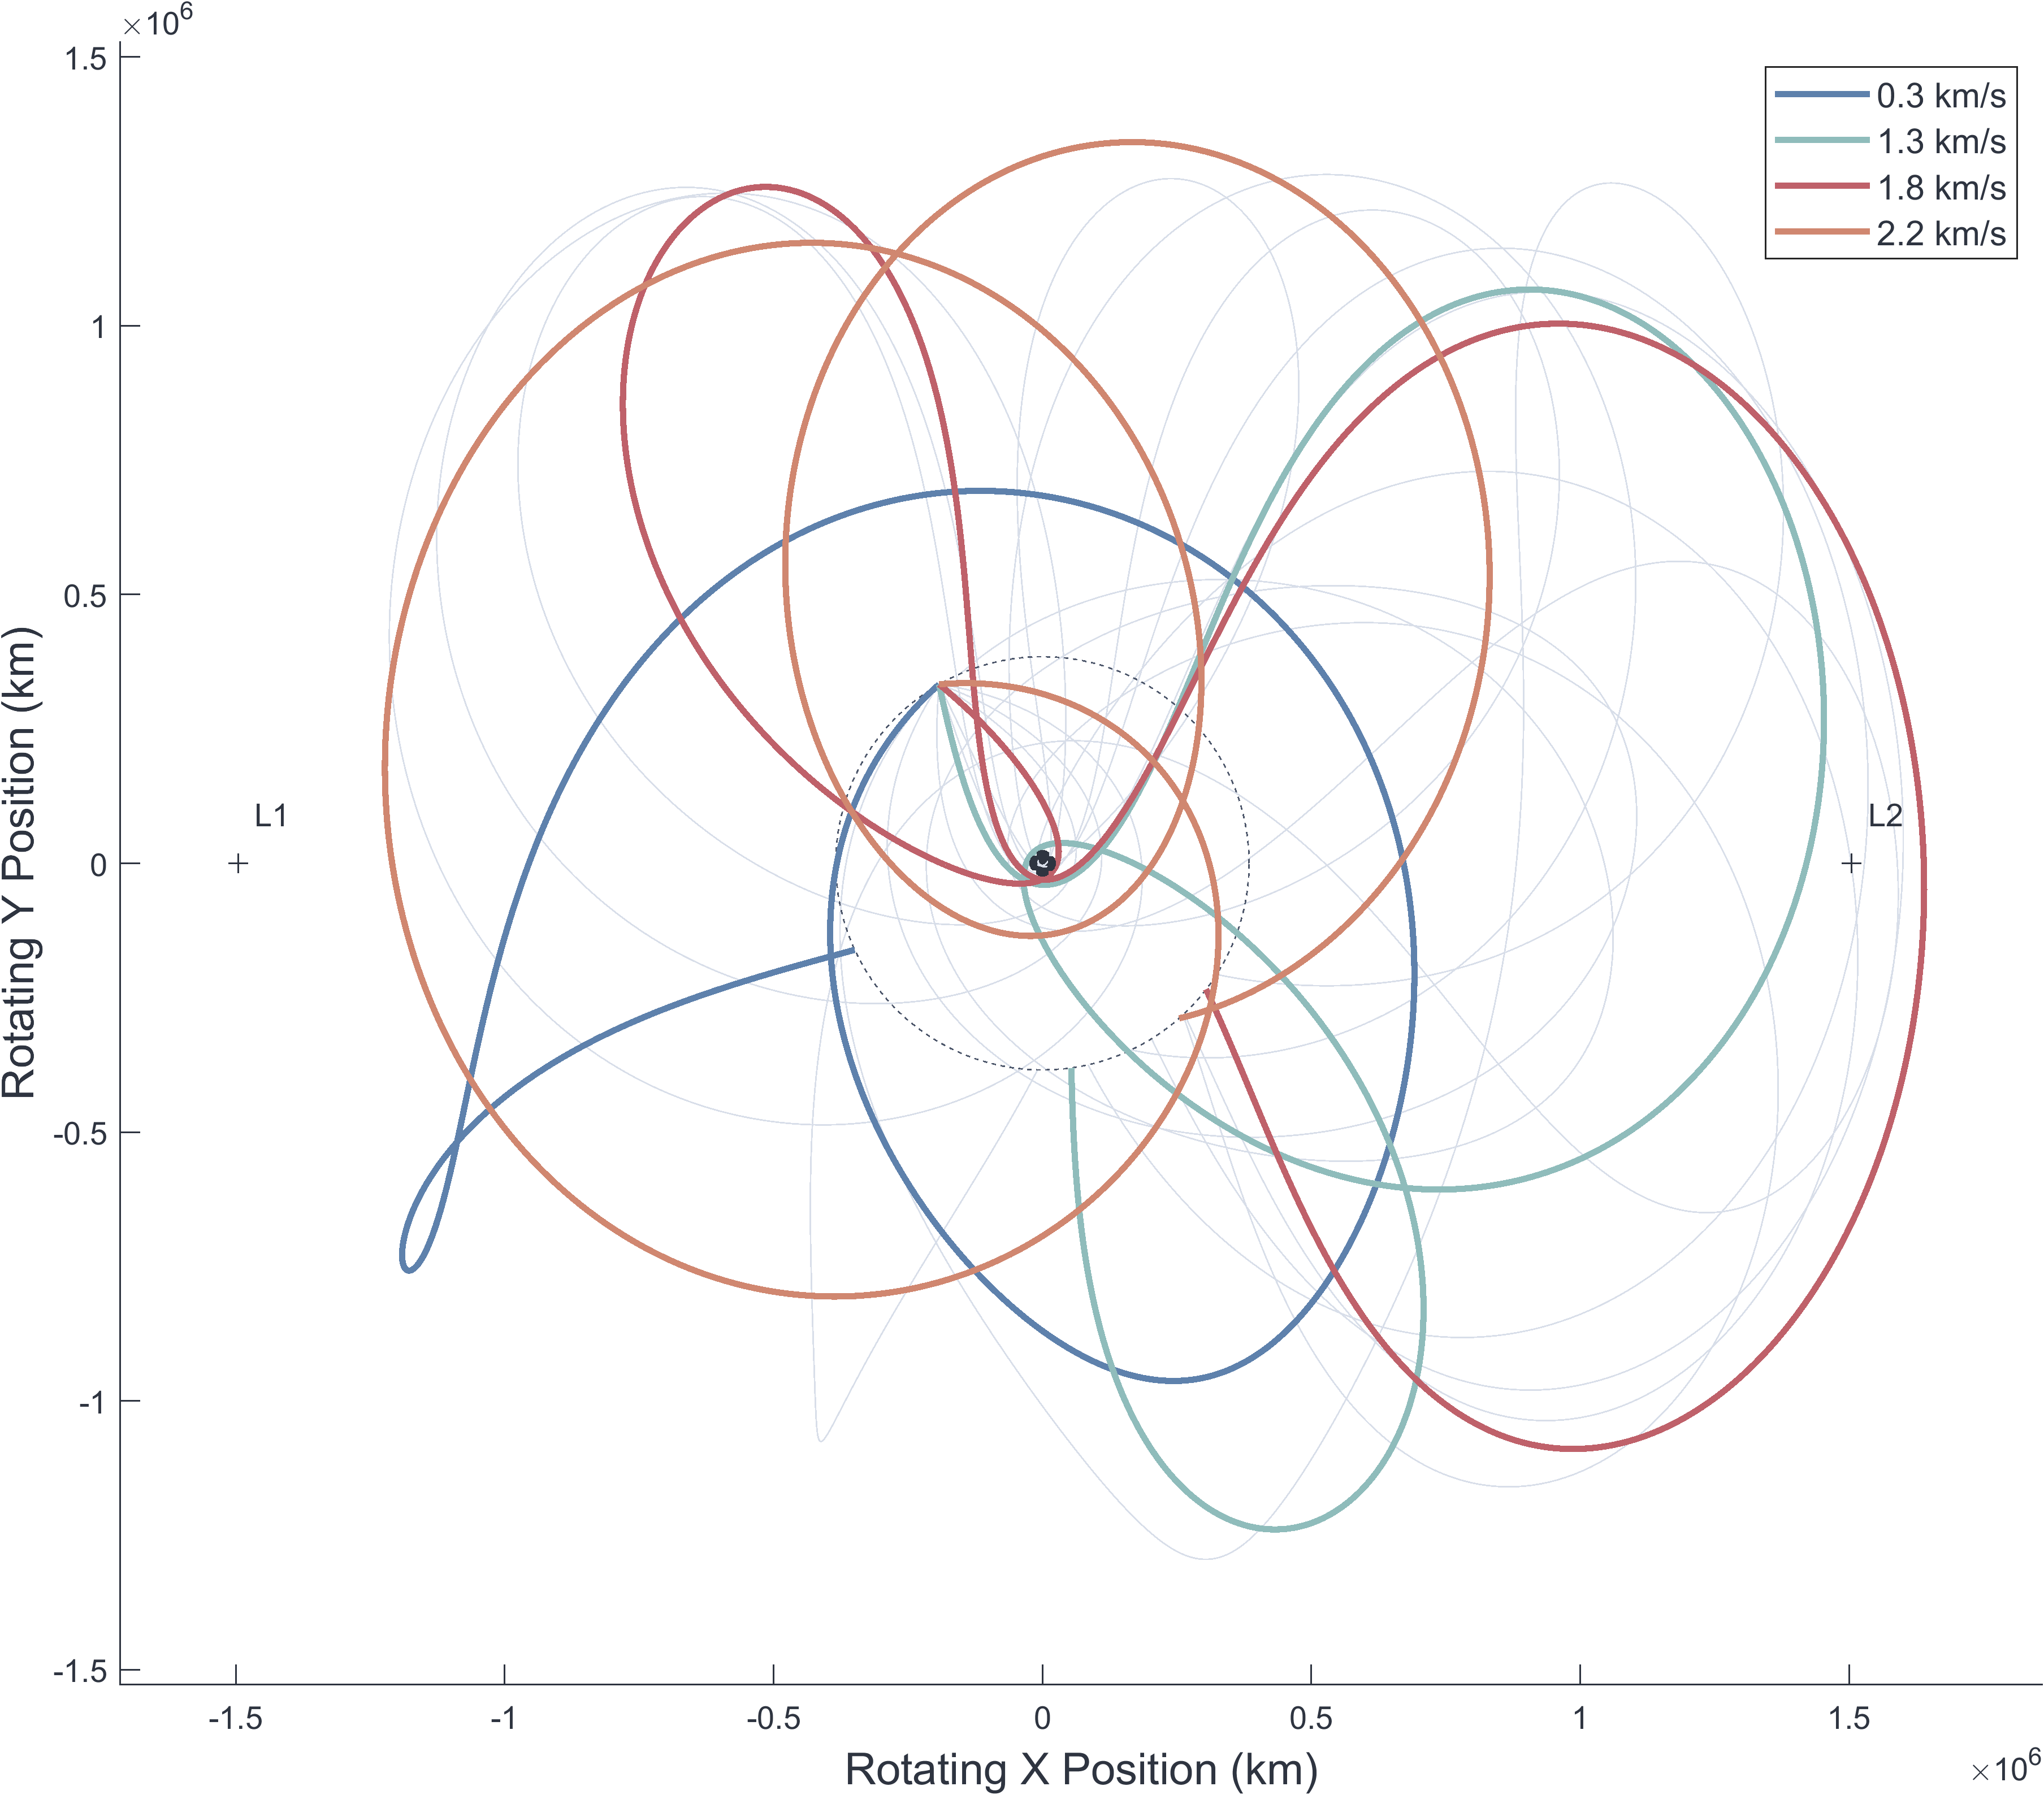
\includegraphics[trim=75 50 0 0, clip, width=3in]{./figs/sunrot_vInfPlot_ii_famF_theta120.png}
    \caption{Progression of Fii family orbits as v\(_\infty\) is increased across initial Solar Phase Angles, \(\theta_0\), of 0°, 60°, and 120°. Similar to the inertial plots, as v\(_\infty\) increases, the orbit trends towards an increasingly retrograde starting path from the Moon.}
    \label{fig:sunrot_vinfPlot_ii_F}
\end{figure}


\begin{figure}[h!]
    \begin{subfigure}{}
        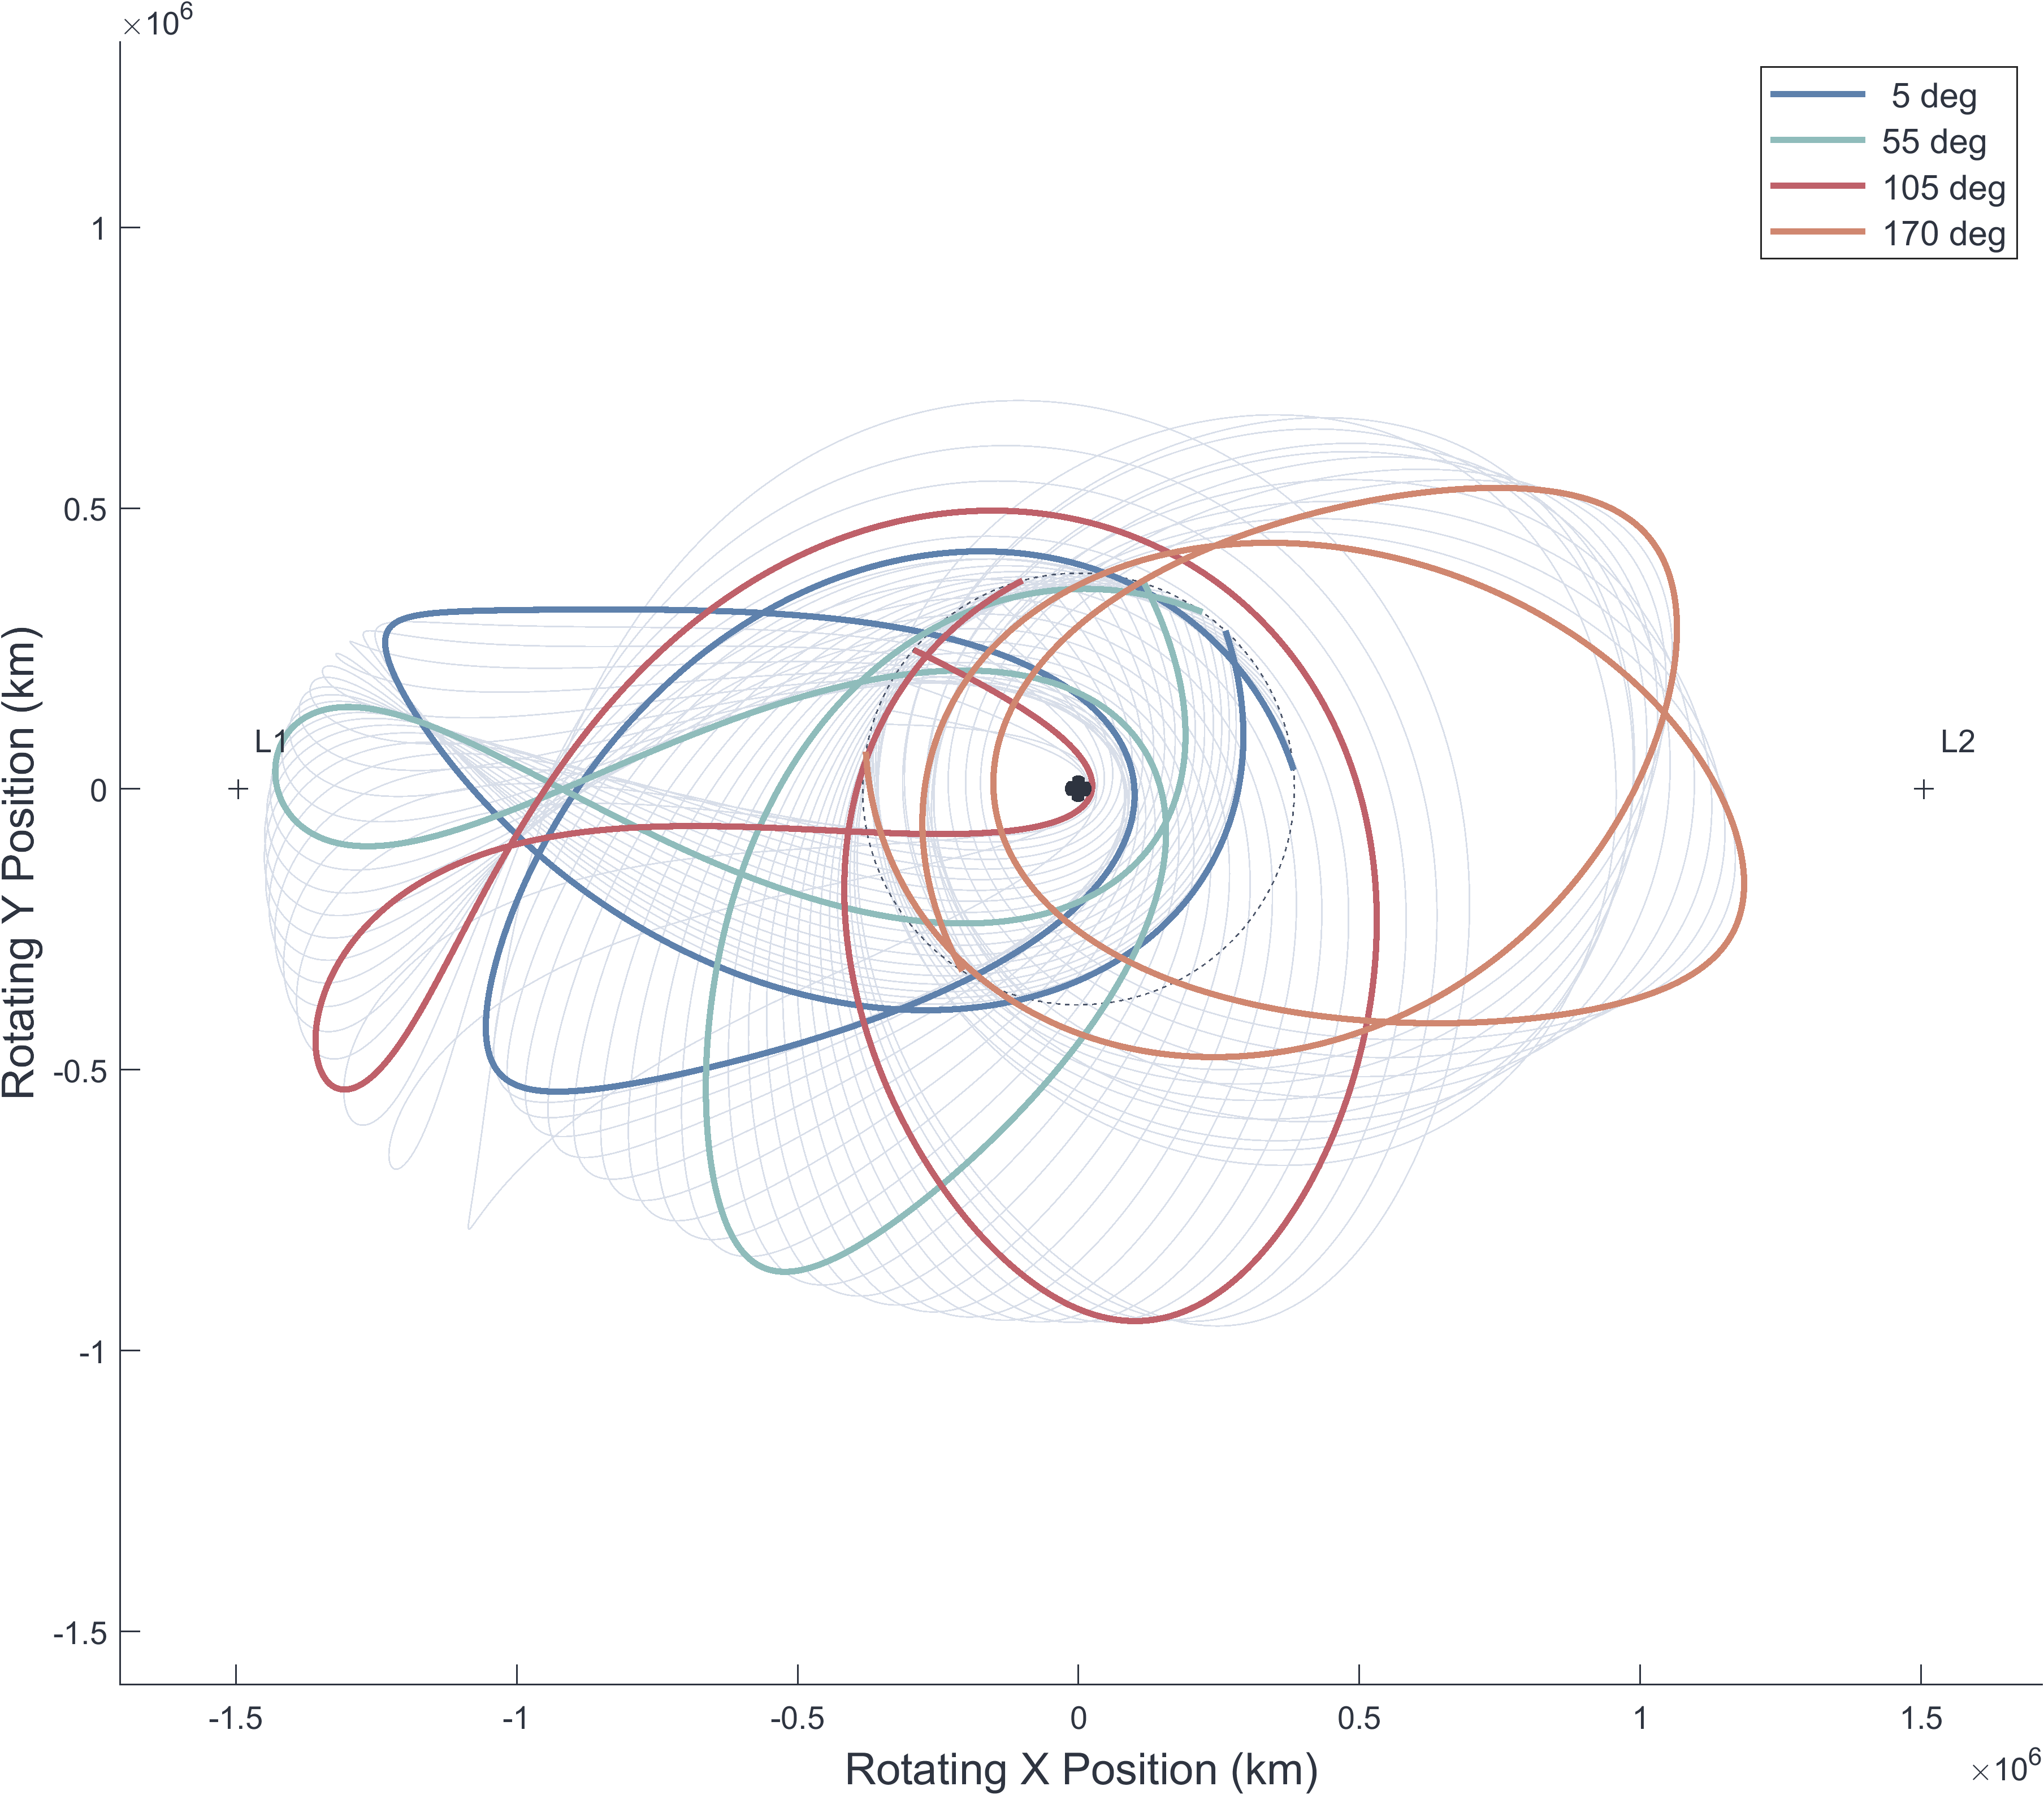
\includegraphics[trim=70 50 0 0, clip, width=2.75in]{./figs/sunrot_ThetaPlot_io_famF_vInf0.3.png}
        % \caption{Top 25 results from Europa Clipper dataset, color sorted by sequence}
    \end{subfigure}
    \begin{subfigure}{}
        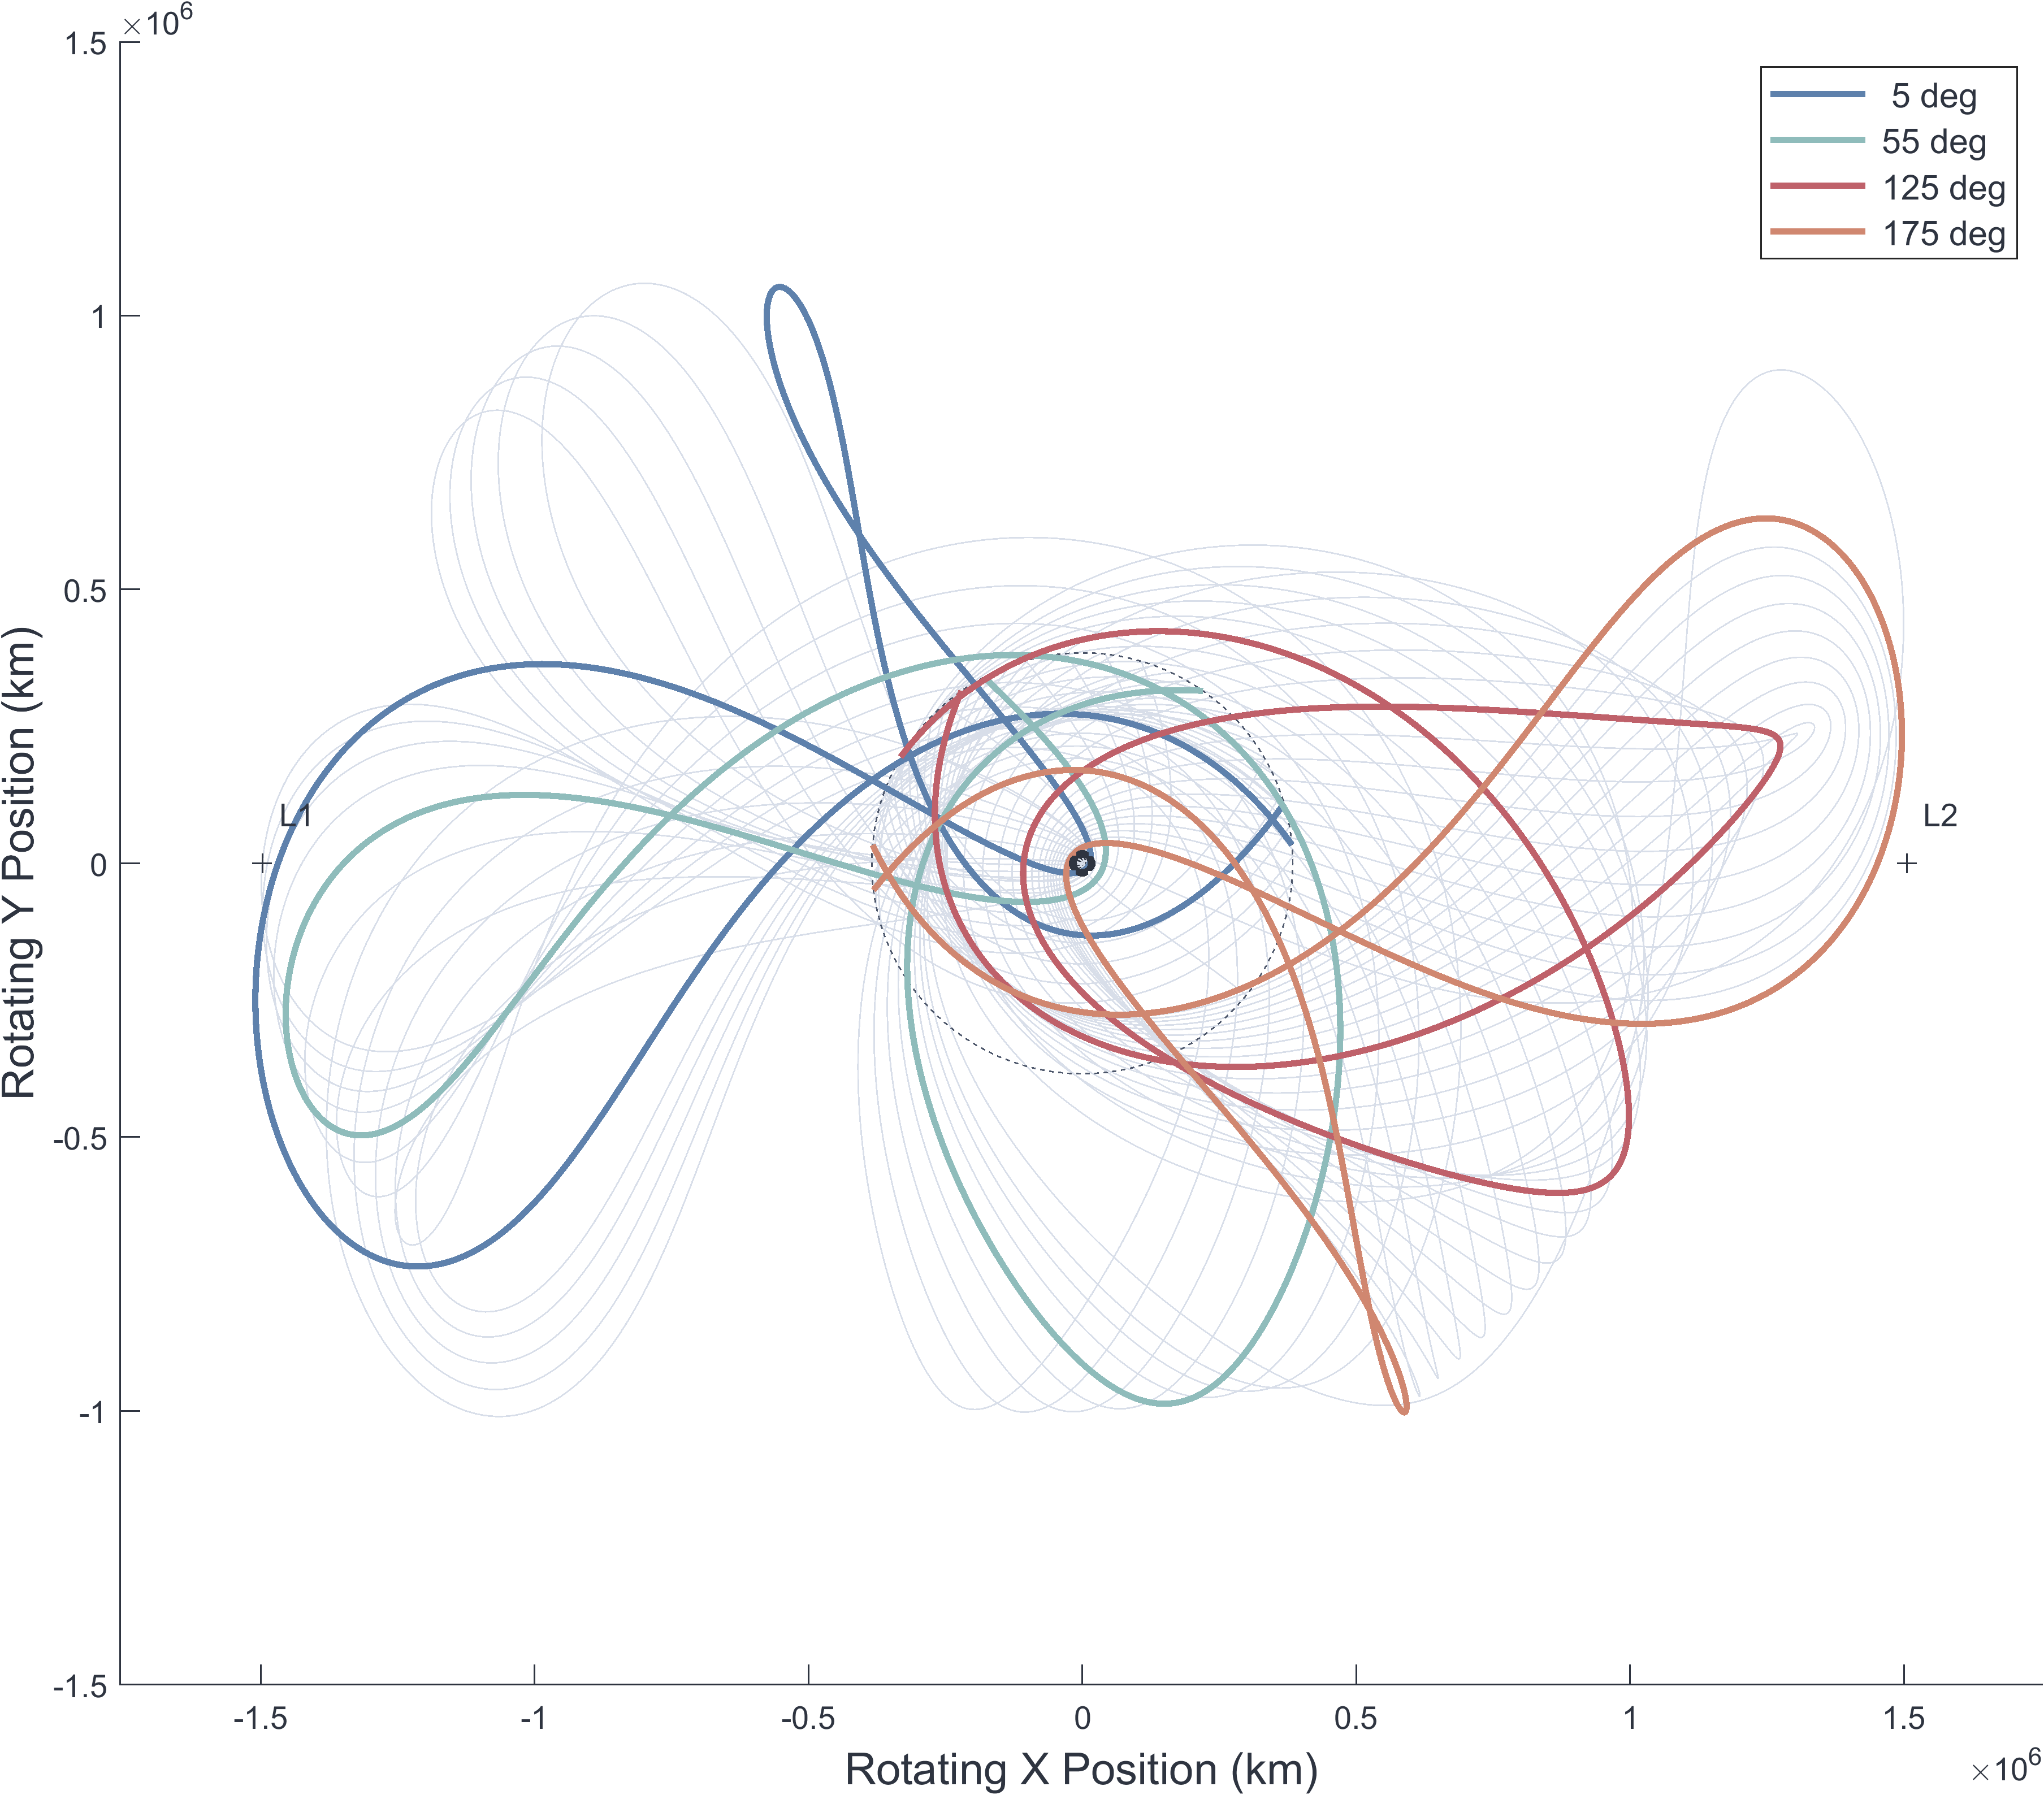
\includegraphics[trim=75 50 0 0, clip, width=2.75in]{./figs/sunrot_ThetaPlot_io_famF_vInf0.6.png}
        % \caption{Top 12 results from Galileo dataset, color sorted by sequence}
    \end{subfigure}
\end{figure}
% \vspace{-5cm}
\begin{figure}[h!]
    \begin{subfigure}{}
        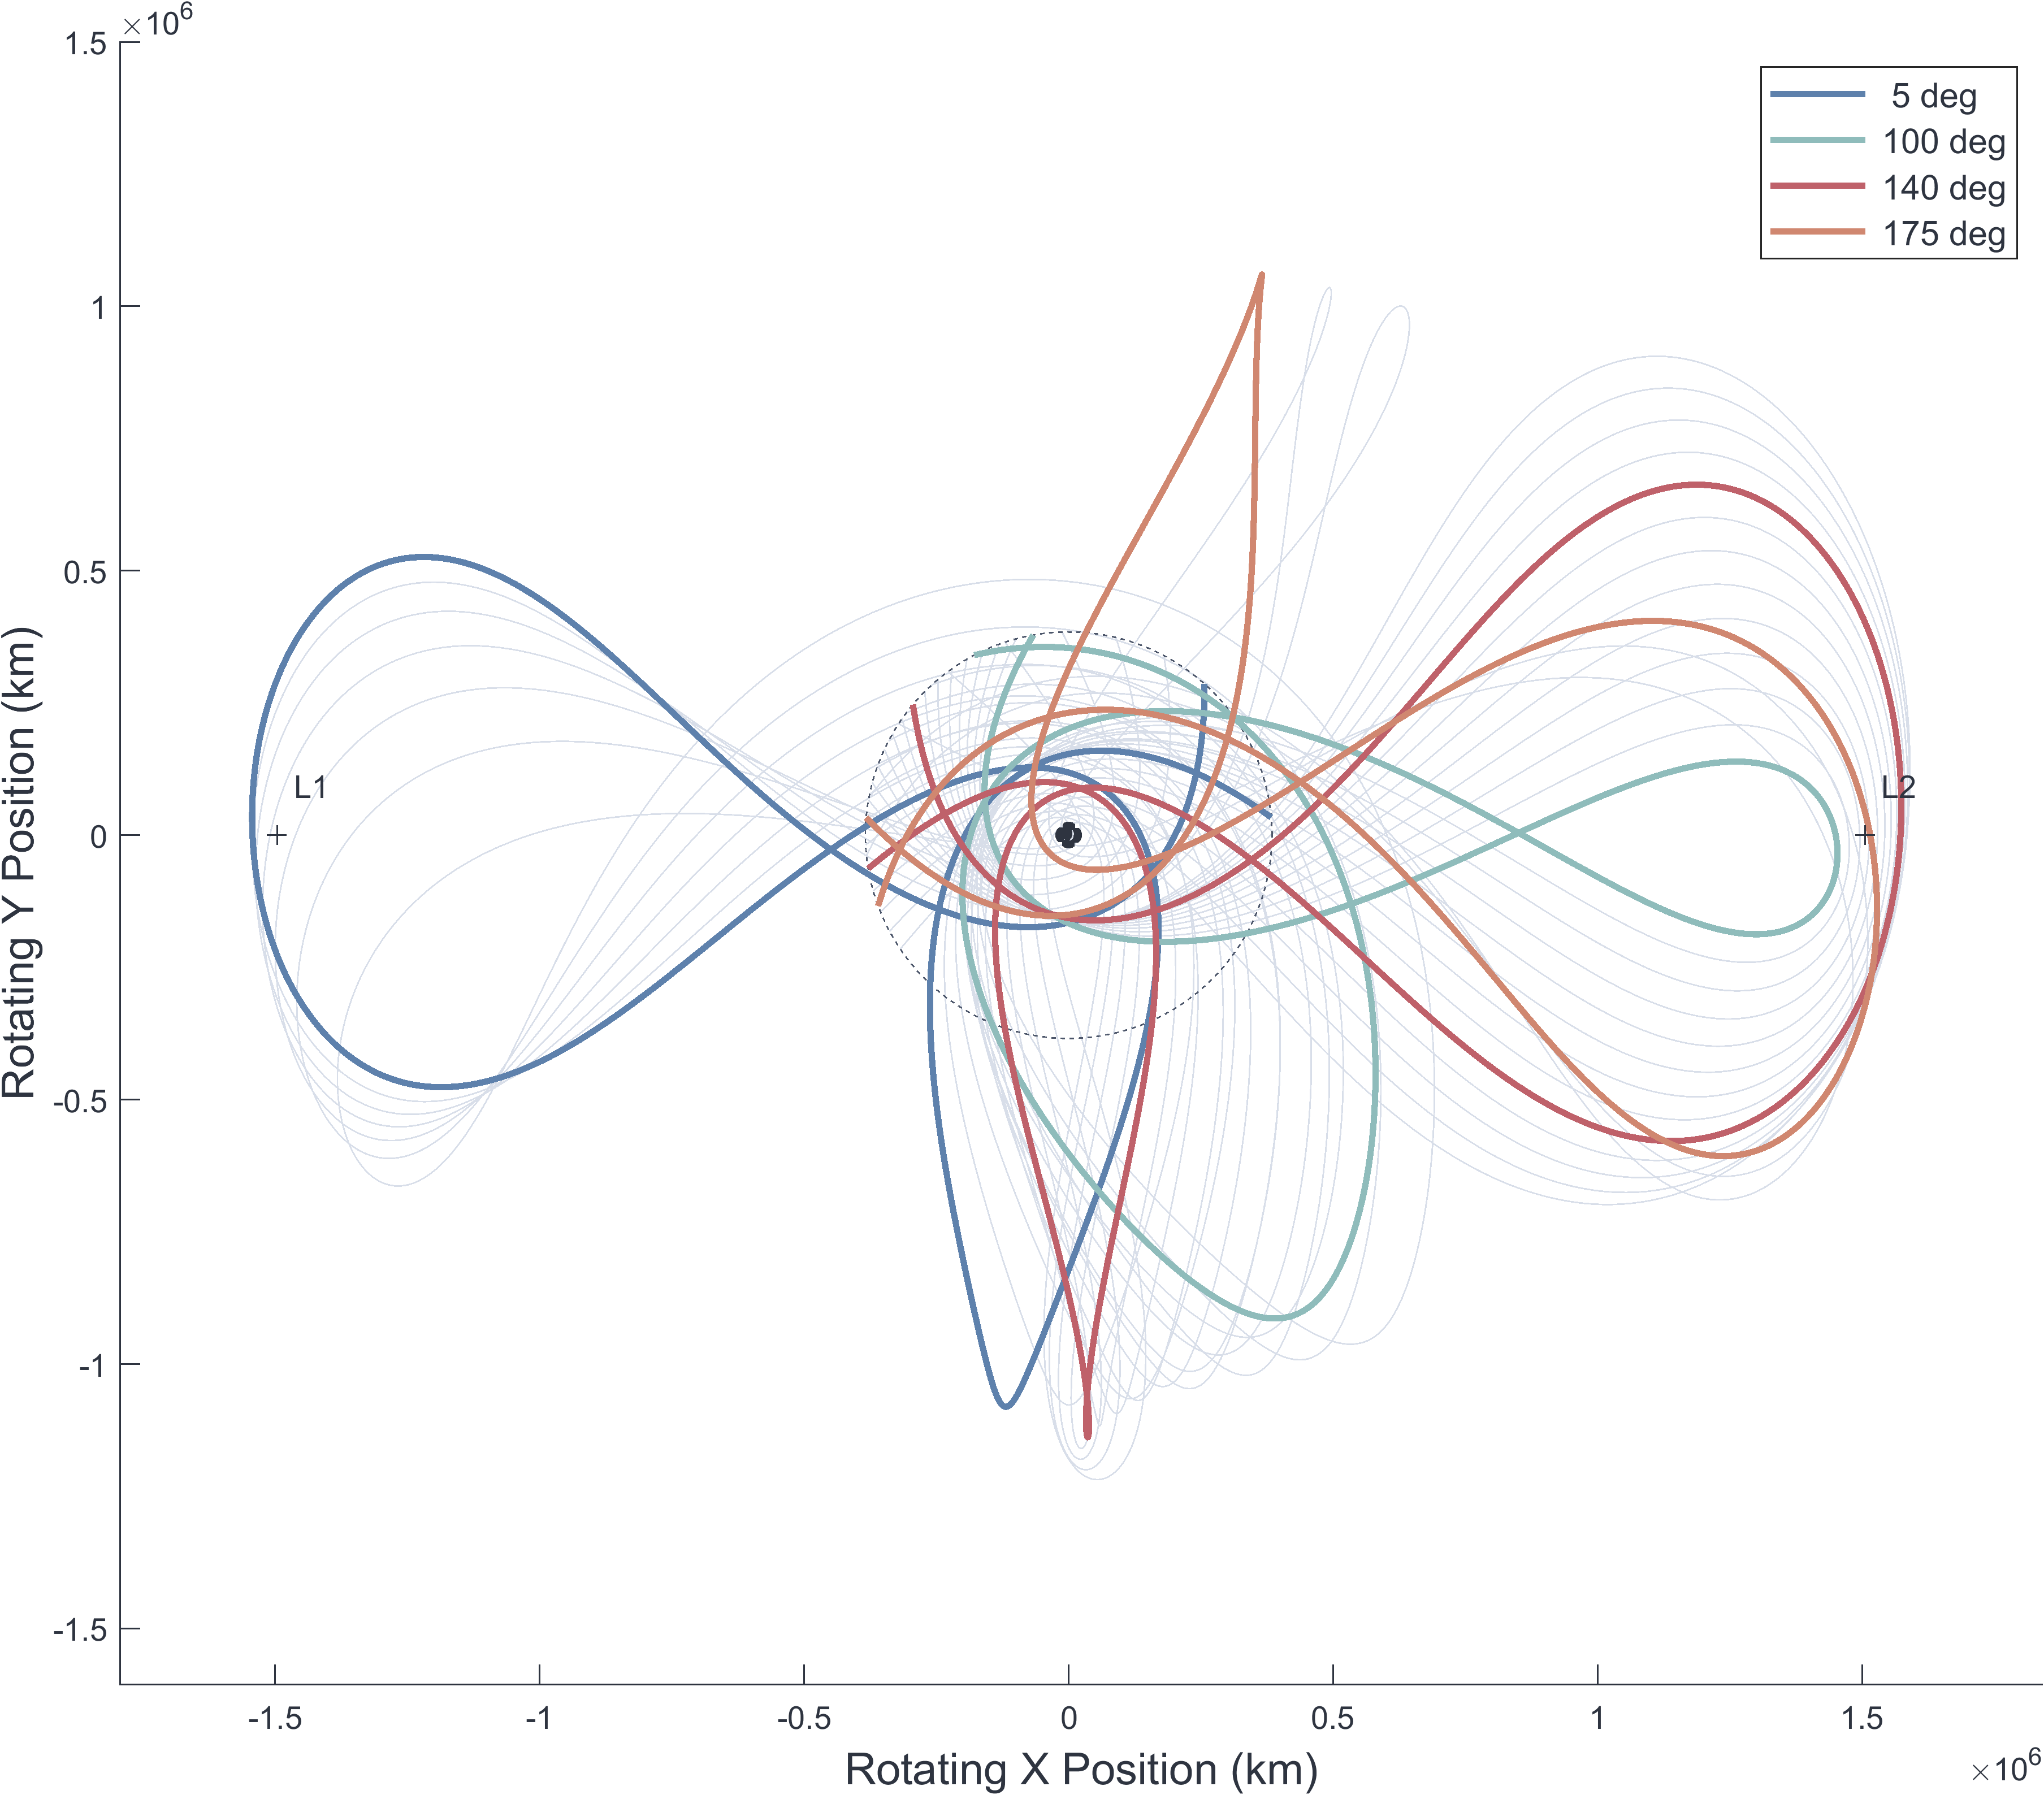
\includegraphics[trim=75 50 0 0, clip, width=2.75in]{./figs/sunrot_ThetaPlot_io_famF_vInf0.9.png}
        % \caption{Top 25 results from Europa Clipper dataset, color sorted by sequence}
    \end{subfigure}
    \begin{subfigure}{}
        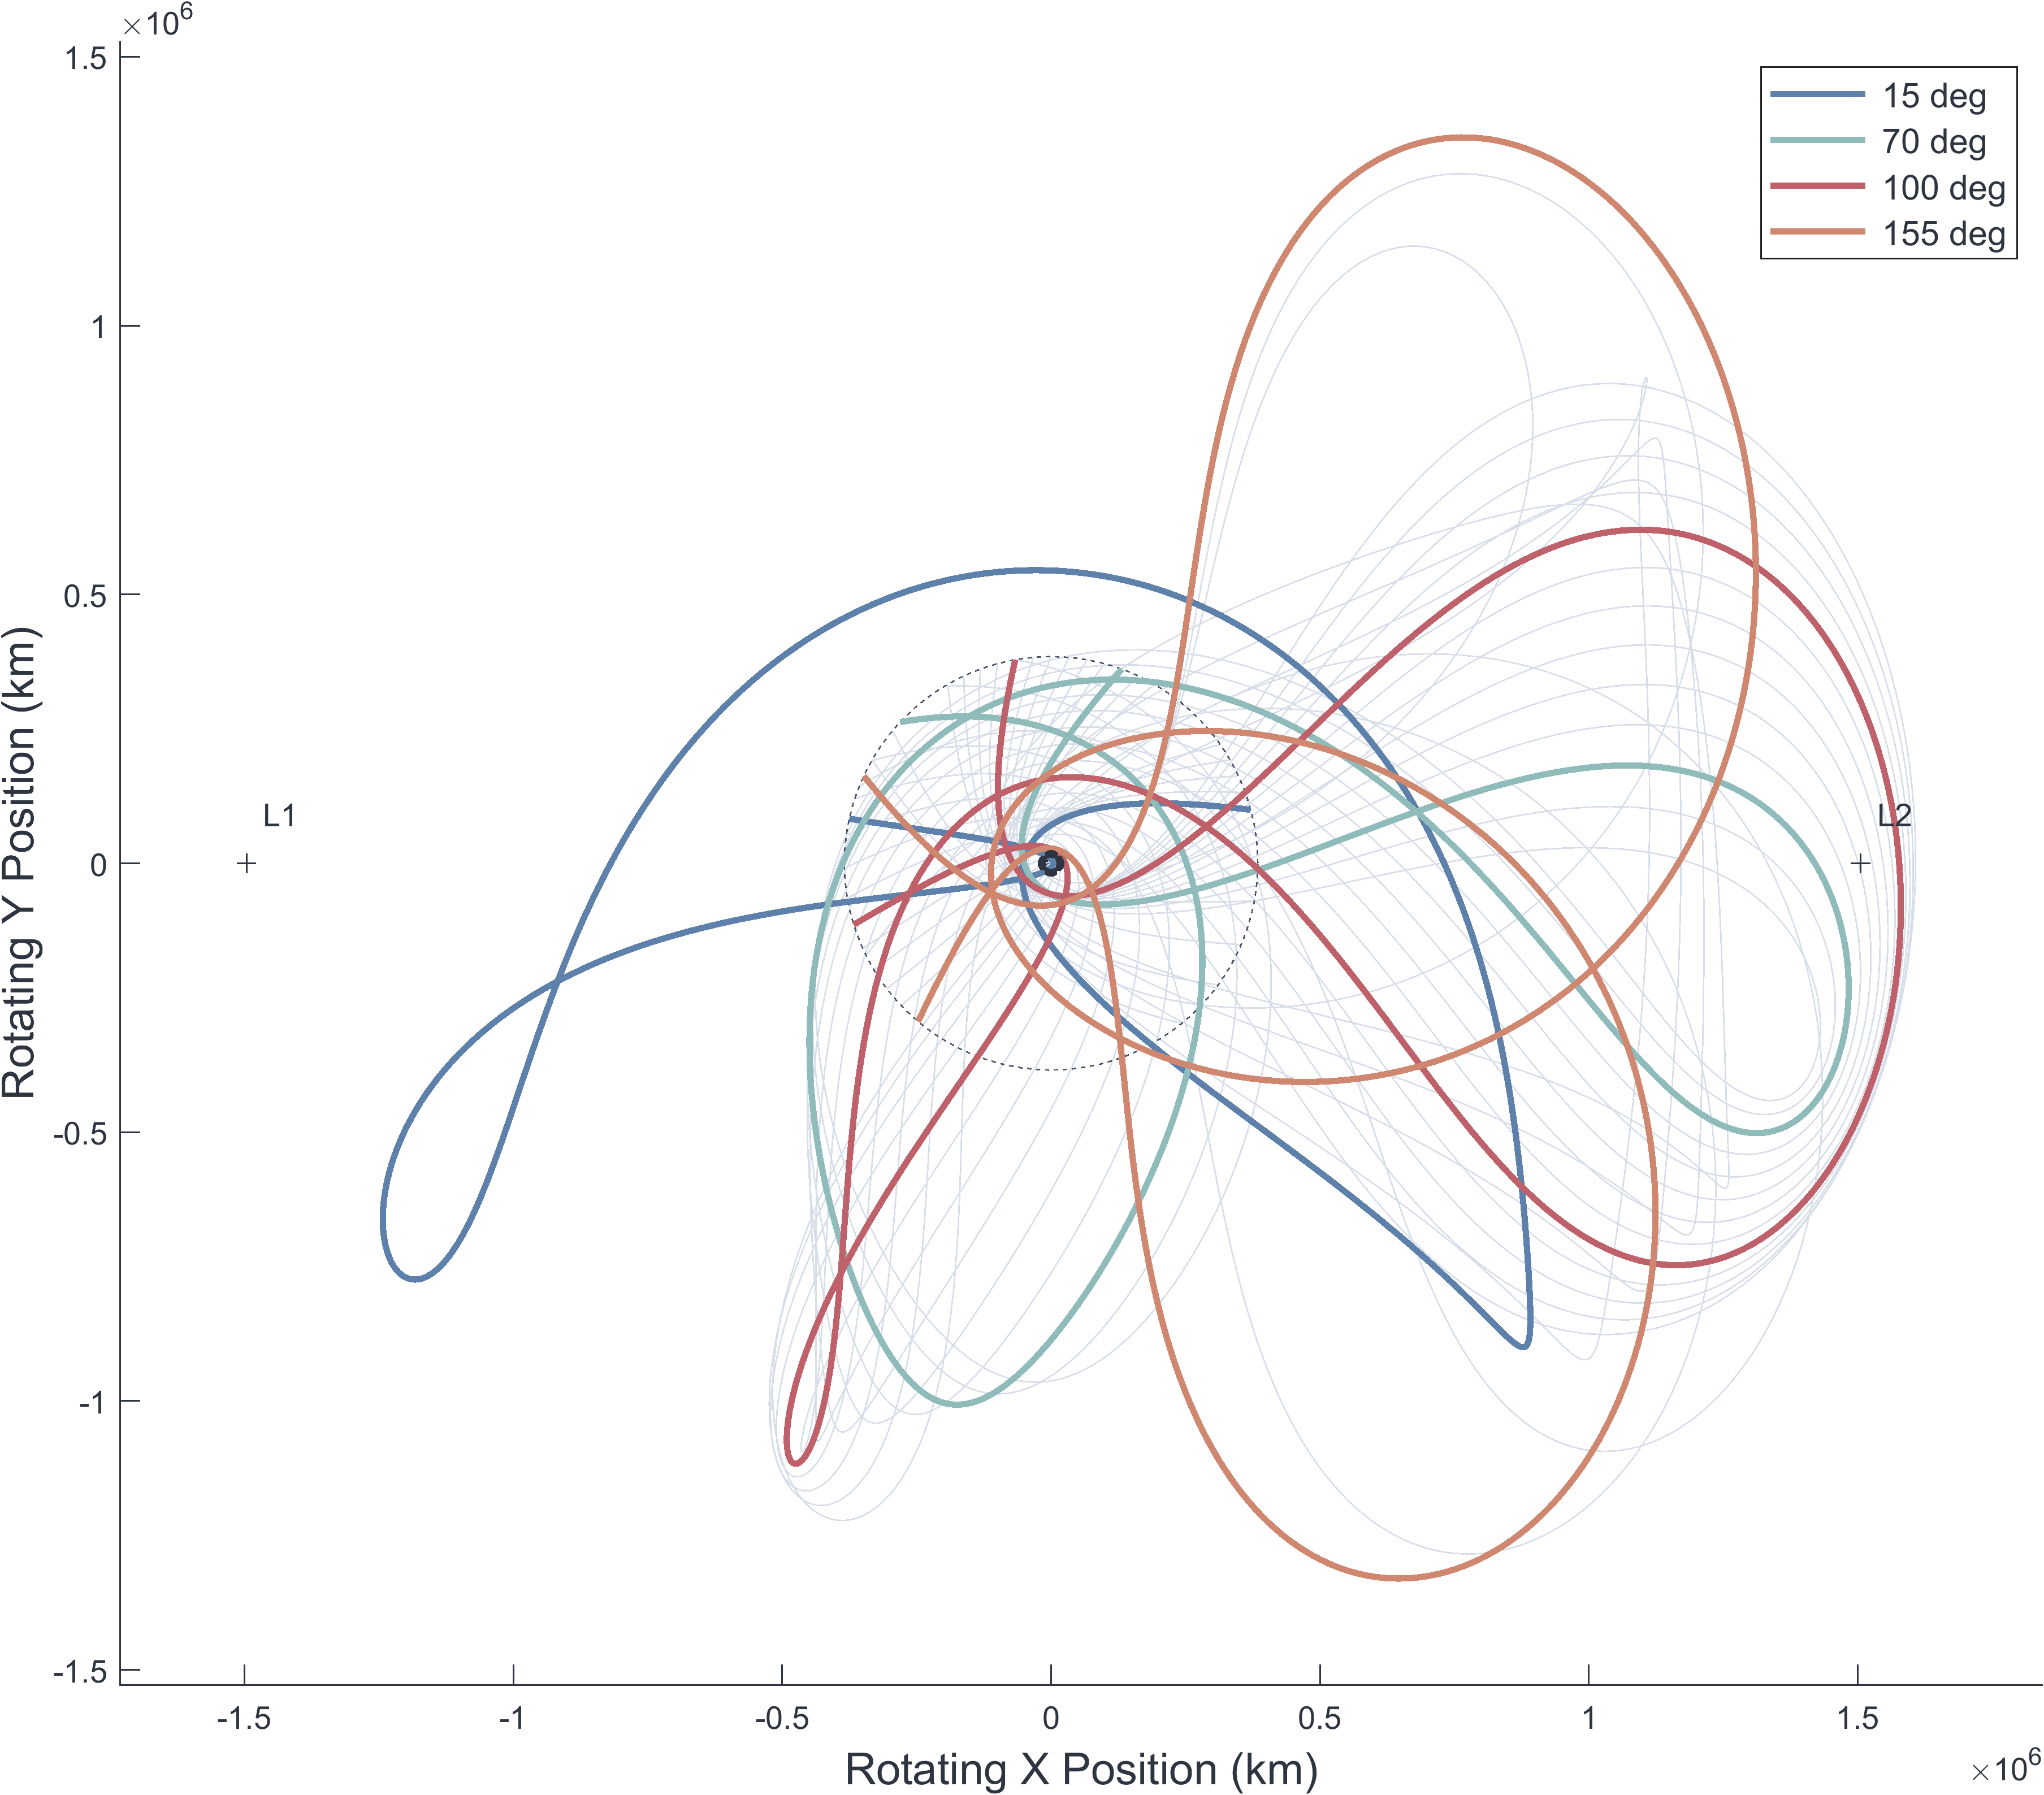
\includegraphics[trim=75 50 0 0, clip, width=2.75in]{./figs/sunrot_ThetaPlot_io_famF_vInf1.2.png}
        % \caption{Top 12 results from Galileo dataset, color sorted by sequence}
    \end{subfigure}
\end{figure}
% \vspace{-5cm}
\begin{figure}[h!]
    \begin{subfigure}{}
        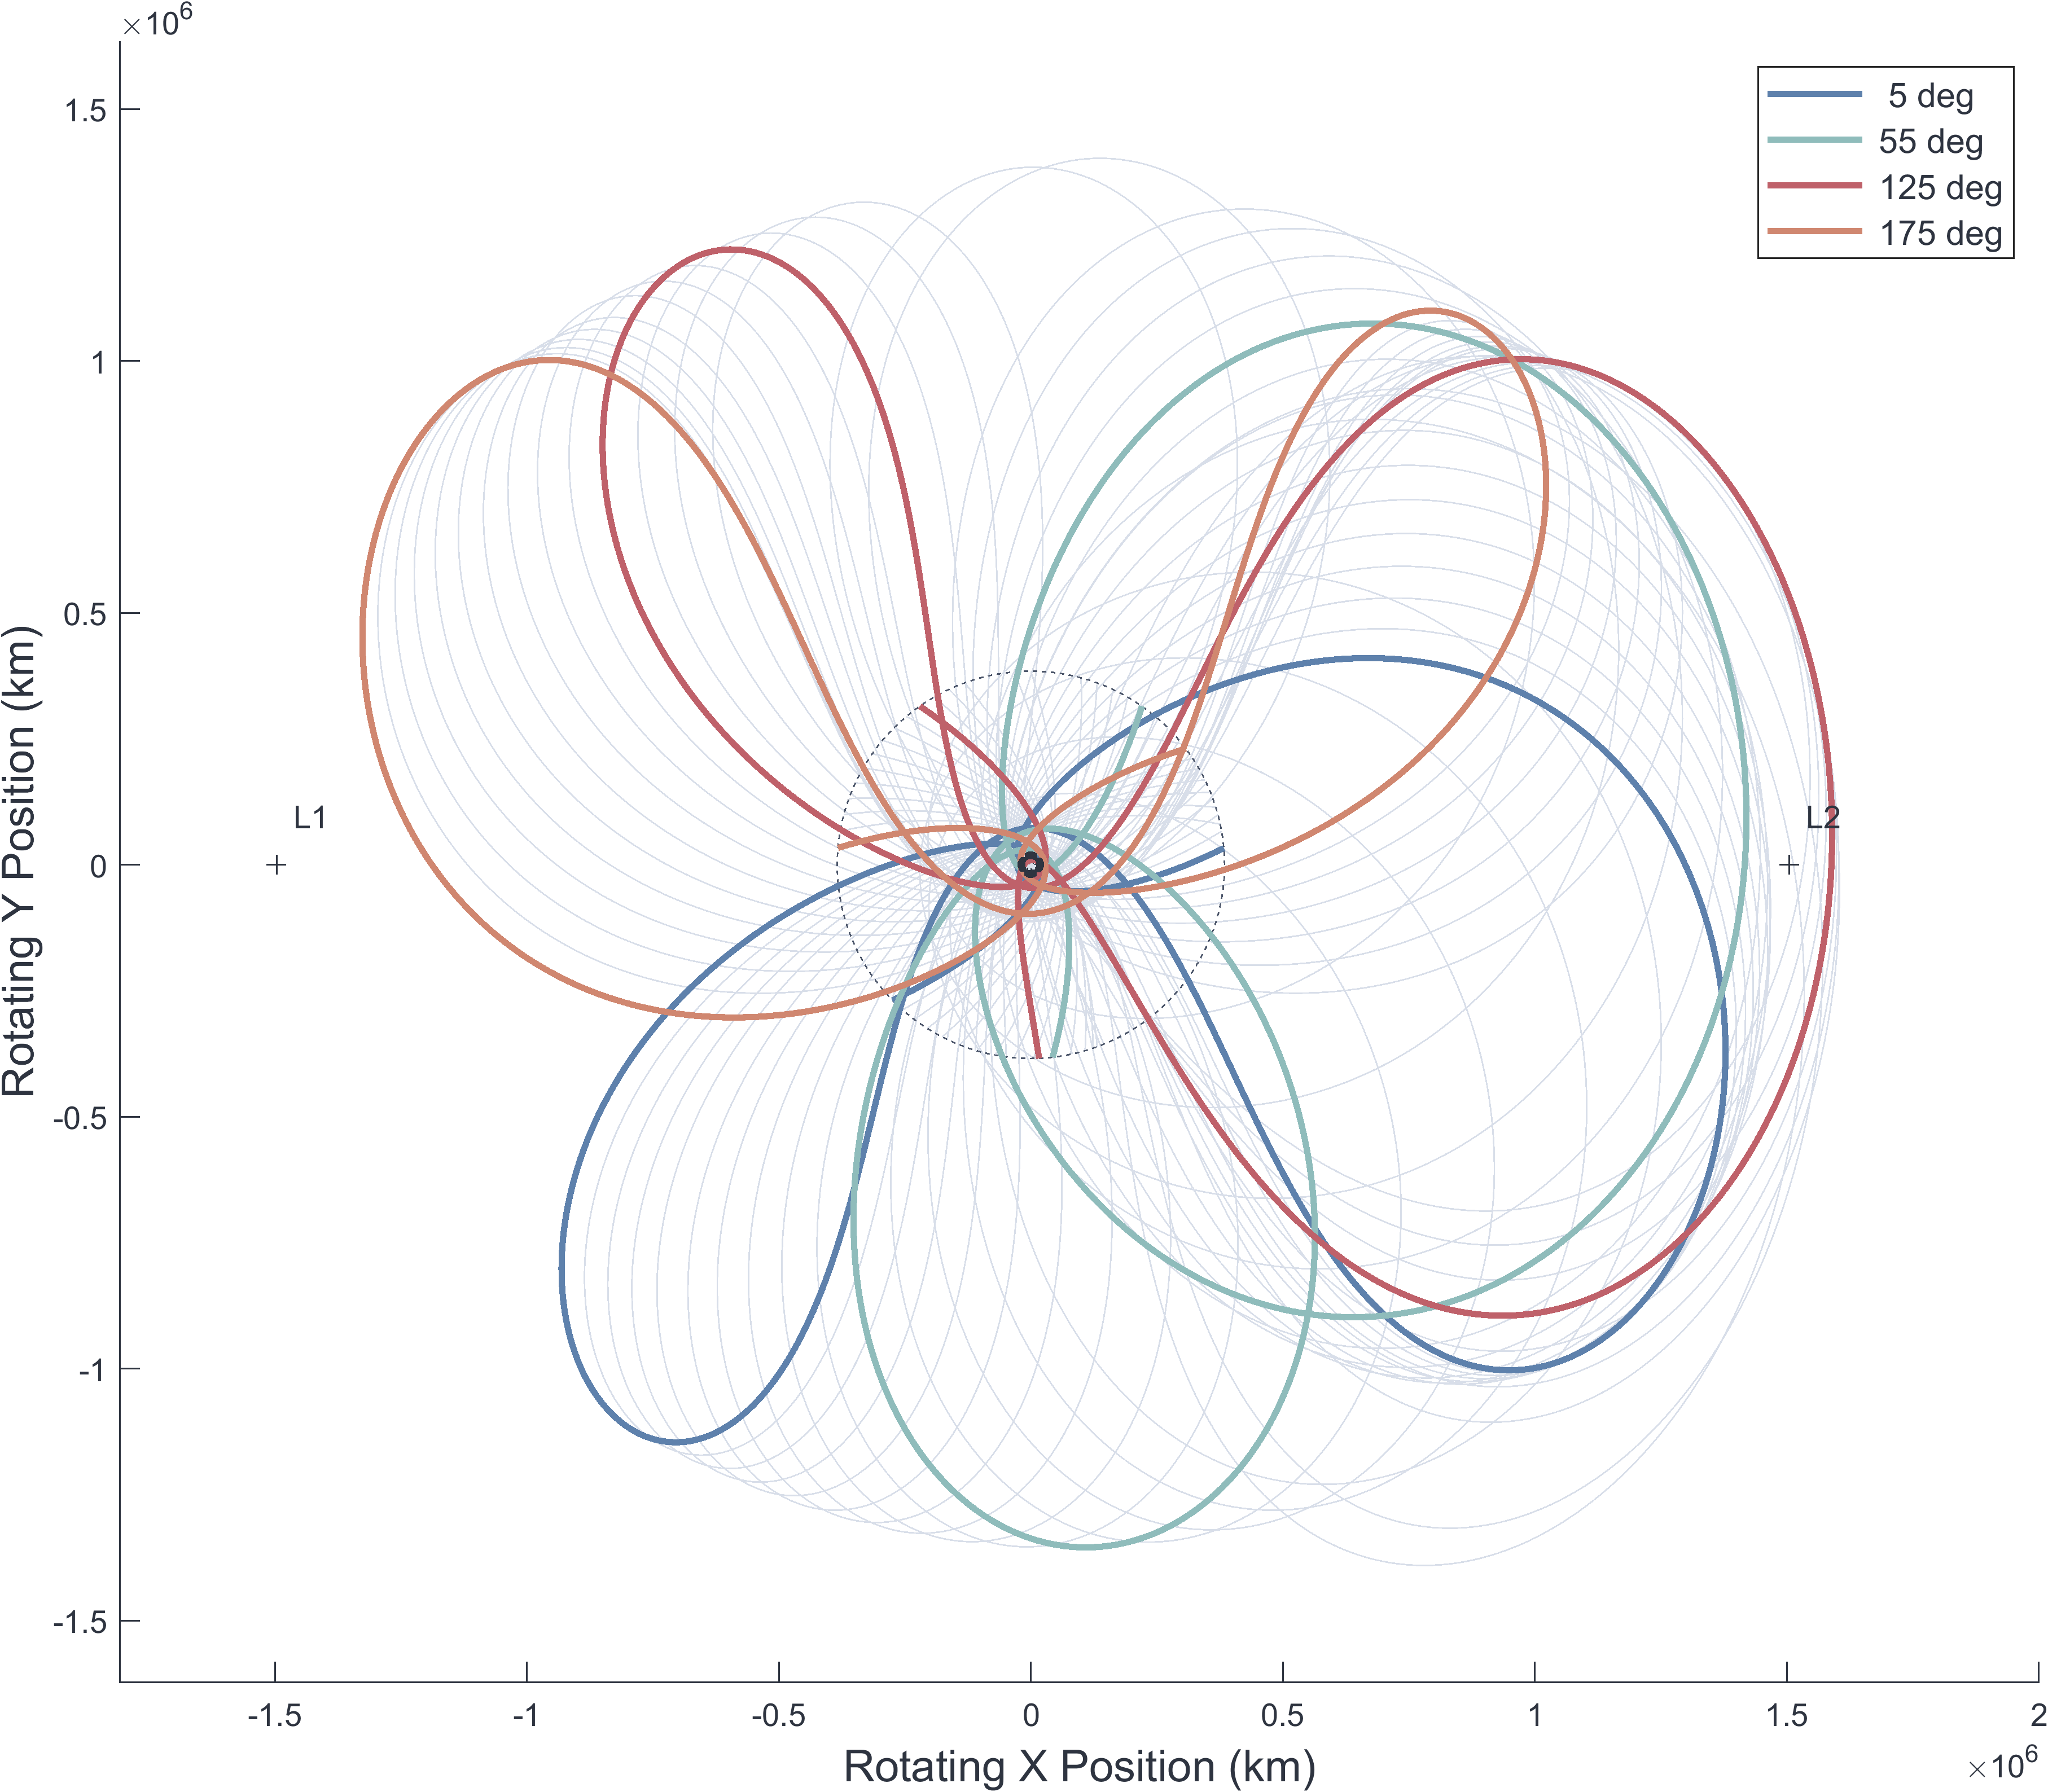
\includegraphics[trim=75 50 0 0, clip, width=2.75in]{./figs/sunrot_ThetaPlot_io_famF_vInf1.8.png}
        % \caption{Top 25 results from Europa Clipper dataset, color sorted by sequence}
    \end{subfigure}
    \begin{subfigure}{}
        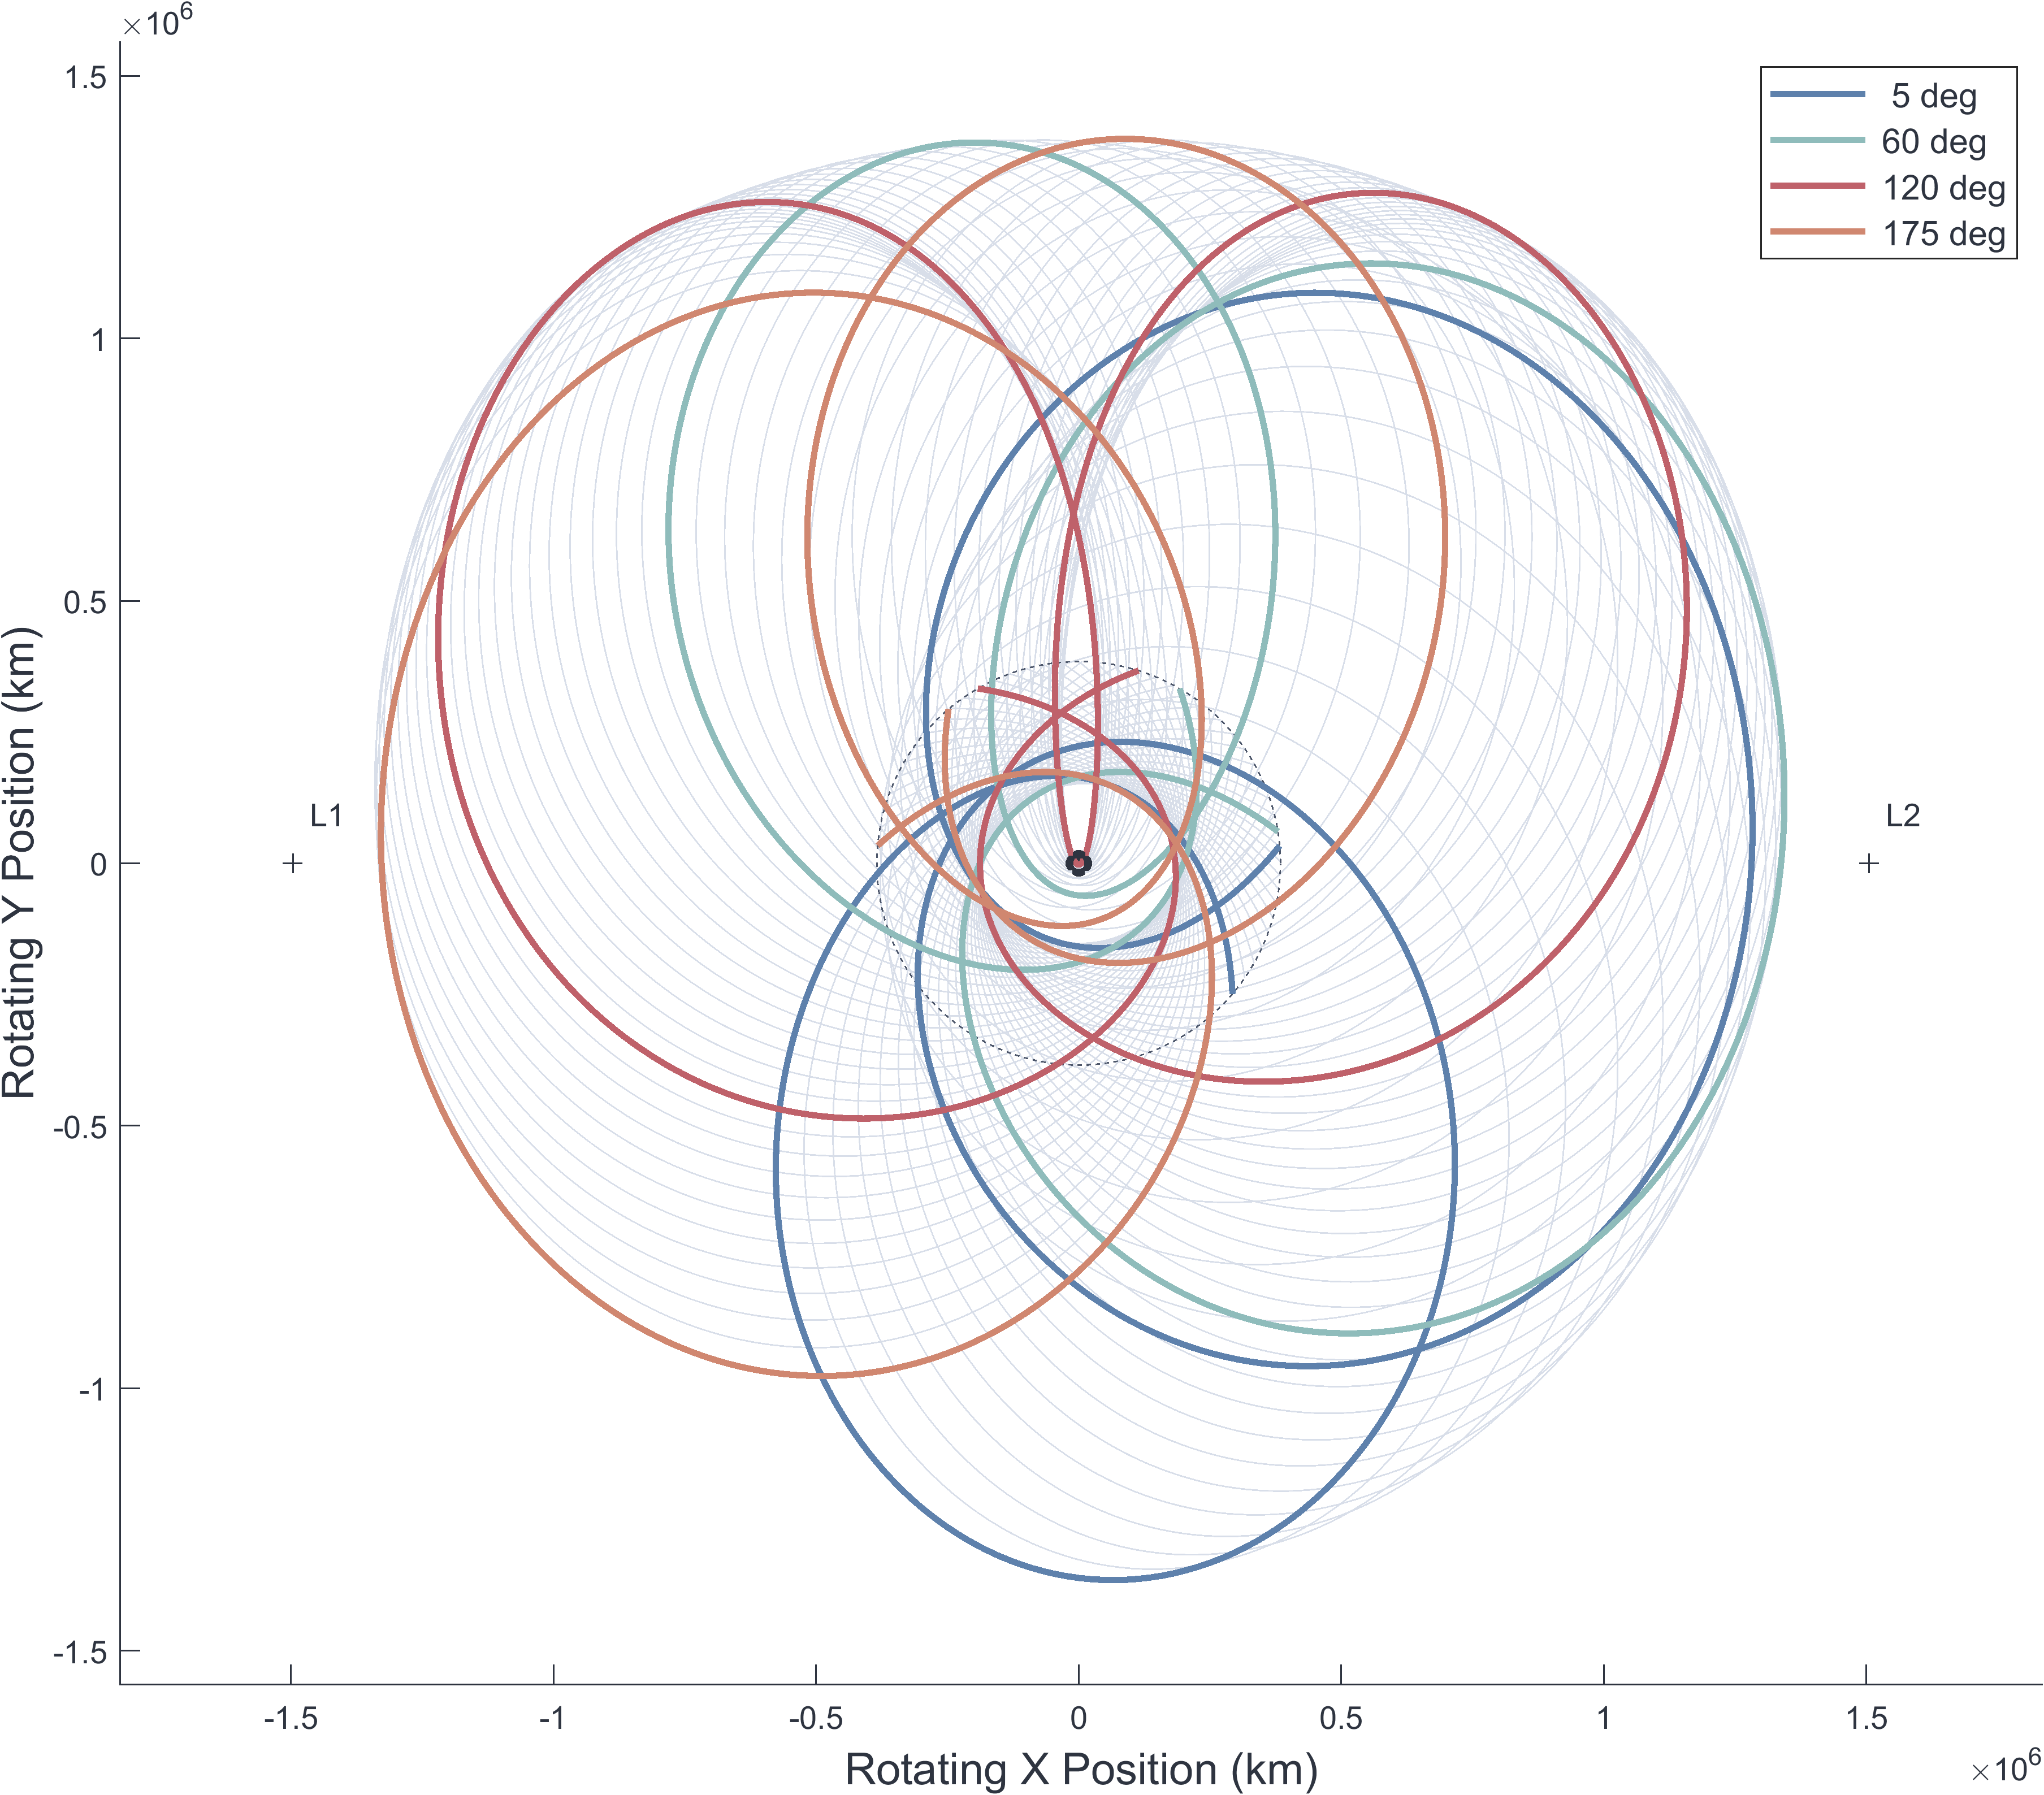
\includegraphics[trim=75 50 0 0, clip, width=2.75in]{./figs/sunrot_ThetaPlot_io_famF_vInf2.1.png}
        % \caption{Top 12 results from Galileo dataset, color sorted by sequence}
    \end{subfigure}
    \caption{Progression of Fio family orbits at a v\(_\infty\)'s of [0.3, 0.6, 0.9, 1.2, 1.8, 2.1] \(^{km}/_s\) (left to right, top to bottom) as the initial Solar Phase Angles, \(\theta_0\), increases. The mirrored structure can be seen as the orbits at 0° and 175° have extremely similar characteristics.}
    \label{fig:sunrot_thetaPlot_io_F_2.1}
\end{figure}

\clearpage

% \section*{Appendix B: Inertial Earth-Centered NEA Scout Trajectory Example}


% \clearpage


\pdfbookmark[1]{References}{ref}
\bibliographystyle{AAS_publication}   % Number the references.
\bibliography{references}   % Use references.bib to resolve the labels.

\end{document}
